\documentclass[authoryearcitations]{UoYCSproject}

\usepackage[includefoot,driver=pdftex,footskip=8mm,top=2cm,inner=2cm,bottom=1cm,outer=1cm]{geometry}
\usepackage[matrix,frame,arrow]{xypic}
\usepackage{titlesec}
\usepackage{scrpage}
\ifx\pdftexversion\undefined
\usepackage[dvips]{graphicx}
\else
\usepackage[pdftex]{graphicx}
\DeclareGraphicsRule{*}{mps}{*}{}
\fi
\usepackage{array}
\usepackage{qtree}
\usepackage{listings}
\usepackage{appendix}
\usepackage{color}
\usepackage{longtable} 
\usepackage{subfigure}
\usepackage{emp}
\usepackage{pdflscape}
\usepackage{algorithm}
\usepackage{algorithmic}
\usepackage[utf8]{inputenc}
\usepackage{hyperref}
% \usepackage[upright]{fourier}
\usepackage{tikz}
\usetikzlibrary{matrix,arrows,decorations.pathmorphing}
%    Q-circuit version 1.2
%    Copyright (C) 2004  Steve Flammia & Bryan Eastin, 4/23/06
%    This program is free software; you can redistribute it and/or modify
%    it under the terms of the GNU General Public License as published by
%    the Free Software Foundation; either version 2 of the License, or
%    (at your option) any later version.
%
%    This program is distributed in the hope that it will be useful,
%    but WITHOUT ANY WARRANTY; without even the implied warranty of
%    MERCHANTABILITY or FITNESS FOR A PARTICULAR PURPOSE.  See the
%    GNU General Public License for more details.
%
%    You should have received a copy of the GNU General Public License
%    along with this program; if not, write to the Free Software
%    Foundation, Inc., 59 Temple Place, Suite 330, Boston, MA  02111-1307  USA

\usepackage[matrix,frame,arrow]{xy}
\usepackage{amsmath}
\newcommand{\bra}[1]{\left\langle{#1}\right\vert}
\newcommand{\ket}[1]{\left\vert{#1}\right\rangle}
    % Defines Dirac notation.
\newcommand{\qw}[1][-1]{\ar @{-} [0,#1]}
    % Defines a wire that connects horizontally.  By default it connects to the object on the left of the current object.
    % WARNING: Wire commands must appear after the gate in any given entry.
\newcommand{\qwx}[1][-1]{\ar @{-} [#1,0]}
    % Defines a wire that connects vertically.  By default it connects to the object above the current object.
    % WARNING: Wire commands must appear after the gate in any given entry.
\newcommand{\cw}[1][-1]{\ar @{=} [0,#1]}
    % Defines a classical wire that connects horizontally.  By default it connects to the object on the left of the current object.
    % WARNING: Wire commands must appear after the gate in any given entry.
\newcommand{\cwx}[1][-1]{\ar @{=} [#1,0]}
    % Defines a classical wire that connects vertically.  By default it connects to the object above the current object.
    % WARNING: Wire commands must appear after the gate in any given entry.
\newcommand{\gate}[1]{*{\xy *+<.6em>{#1};p\save+LU;+RU **\dir{-}\restore\save+RU;+RD **\dir{-}\restore\save+RD;+LD **\dir{-}\restore\POS+LD;+LU **\dir{-}\endxy} \qw}
    % Boxes the argument, making a gate.
\newcommand{\meter}{\gate{\xy *!<0em,1.1em>h\cir<1.1em>{ur_dr},!U-<0em,.4em>;p+<.5em,.9em> **h\dir{-} \POS <-.6em,.4em> *{},<.6em,-.4em> *{} \endxy}}
    % Inserts a measurement meter.
\newcommand{\measure}[1]{*+[F-:<.9em>]{#1} \qw}
    % Inserts a measurement bubble with user defined text.
\newcommand{\measuretab}[1]{*{\xy *+<.6em>{#1};p\save+LU;+RU **\dir{-}\restore\save+RU;+RD **\dir{-}\restore\save+RD;+LD **\dir{-}\restore\save+LD;+LC-<.5em,0em> **\dir{-} \restore\POS+LU;+LC-<.5em,0em> **\dir{-} \endxy} \qw}
    % Inserts a measurement tab with user defined text.
\newcommand{\measureD}[1]{*{\xy*+=+<.5em>{\vphantom{\rule{0em}{.1em}#1}}*\cir{r_l};p\save*!R{#1} \restore\save+UC;+UC-<.5em,0em>*!R{\hphantom{#1}}+L **\dir{-} \restore\save+DC;+DC-<.5em,0em>*!R{\hphantom{#1}}+L **\dir{-} \restore\POS+UC-<.5em,0em>*!R{\hphantom{#1}}+L;+DC-<.5em,0em>*!R{\hphantom{#1}}+L **\dir{-} \endxy} \qw}
    % Inserts a D-shaped measurement gate with user defined text.
\newcommand{\multimeasure}[2]{*+<1em,.9em>{\hphantom{#2}} \qw \POS[0,0].[#1,0];p !C *{#2},p \drop\frm<.9em>{-}}
    % Draws a multiple qubit measurement bubble starting at the current position and spanning #1 additional gates below.
    % #2 gives the label for the gate.
    % You must use an argument of the same width as #2 in \ghost for the wires to connect properly on the lower lines.
\newcommand{\multimeasureD}[2]{*+<1em,.9em>{\hphantom{#2}}\save[0,0].[#1,0];p\save !C *{#2},p+LU+<0em,0em>;+RU+<-.8em,0em> **\dir{-}\restore\save +LD;+LU **\dir{-}\restore\save +LD;+RD-<.8em,0em> **\dir{-} \restore\save +RD+<0em,.8em>;+RU-<0em,.8em> **\dir{-} \restore \POS !UR*!UR{\cir<.9em>{r_d}};!DR*!DR{\cir<.9em>{d_l}}\restore \qw}
    % Draws a multiple qubit D-shaped measurement gate starting at the current position and spanning #1 additional gates below.
    % #2 gives the label for the gate.
    % You must use an argument of the same width as #2 in \ghost for the wires to connect properly on the lower lines.
\newcommand{\control}{*!<0em,.025em>-=-{\bullet}}
    % Inserts an unconnected control.
\newcommand{\controlo}{*-<.21em,.21em>{\xy *=<.59em>!<0em,-.02em>[o][F]{}\POS!C\endxy}}
    % Inserts a unconnected control-on-0.
\newcommand{\ctrl}[1]{\control \qwx[#1] \qw}
    % Inserts a control and connects it to the object #1 wires below.
\newcommand{\ctrlo}[1]{\controlo \qwx[#1] \qw}
    % Inserts a control-on-0 and connects it to the object #1 wires below.
\newcommand{\targ}{*!<0em,.019em>=<.79em,.68em>{\xy {<0em,0em>*{} \ar @{ - } +<.4em,0em> \ar @{ - } -<.4em,0em> \ar @{ - } +<0em,.36em> \ar @{ - } -<0em,.36em>},<0em,-.019em>*+<.8em>\frm{o}\endxy} \qw}
    % Inserts a CNOT target.
\newcommand{\qswap}{*=<0em>{\times} \qw}
    % Inserts half a swap gate. 
    % Must be connected to the other swap with \qwx.
\newcommand{\multigate}[2]{*+<1em,.9em>{\hphantom{#2}} \qw \POS[0,0].[#1,0];p !C *{#2},p \save+LU;+RU **\dir{-}\restore\save+RU;+RD **\dir{-}\restore\save+RD;+LD **\dir{-}\restore\save+LD;+LU **\dir{-}\restore}
    % Draws a multiple qubit gate starting at the current position and spanning #1 additional gates below.
    % #2 gives the label for the gate.
    % You must use an argument of the same width as #2 in \ghost for the wires to connect properly on the lower lines.
\newcommand{\ghost}[1]{*+<1em,.9em>{\hphantom{#1}} \qw}
    % Leaves space for \multigate on wires other than the one on which \multigate appears.  Without this command wires will cross your gate.
    % #1 should match the second argument in the corresponding \multigate. 
\newcommand{\push}[1]{*{#1}}
    % Inserts #1, overriding the default that causes entries to have zero size.  This command takes the place of a gate.
    % Like a gate, it must precede any wire commands.
    % \push is useful for forcing columns apart.
    % NOTE: It might be useful to know that a gate is about 1.3 times the height of its contents.  I.e. \gate{M} is 1.3em tall.
    % WARNING: \push must appear before any wire commands and may not appear in an entry with a gate or label.
\newcommand{\gategroup}[6]{\POS"#1,#2"."#3,#2"."#1,#4"."#3,#4"!C*+<#5>\frm{#6}}
    % Constructs a box or bracket enclosing the square block spanning rows #1-#3 and columns=#2-#4.
    % The block is given a margin #5/2, so #5 should be a valid length.
    % #6 can take the following arguments -- or . or _\} or ^\} or \{ or \} or _) or ^) or ( or ) where the first two options yield dashed and
    % dotted boxes respectively, and the last eight options yield bottom, top, left, and right braces of the curly or normal variety.
    % \gategroup can appear at the end of any gate entry, but it's good form to pick one of the corner gates.
    % BUG: \gategroup uses the four corner gates to determine the size of the bounding box.  Other gates may stick out of that box.  See \prop. 
\newcommand{\rstick}[1]{*!L!<-.5em,0em>=<0em>{#1}}
    % Centers the left side of #1 in the cell.  Intended for lining up wire labels.  Note that non-gates have default size zero.
\newcommand{\lstick}[1]{*!R!<.5em,0em>=<0em>{#1}}
    % Centers the right side of #1 in the cell.  Intended for lining up wire labels.  Note that non-gates have default size zero.
\newcommand{\ustick}[1]{*!D!<0em,-.5em>=<0em>{#1}}
    % Centers the bottom of #1 in the cell.  Intended for lining up wire labels.  Note that non-gates have default size zero.
\newcommand{\dstick}[1]{*!U!<0em,.5em>=<0em>{#1}}
    % Centers the top of #1 in the cell.  Intended for lining up wire labels.  Note that non-gates have default size zero.
\newcommand{\Qcircuit}[1][0em]{\xymatrix @*[o] @*=<#1>}
    % Defines \Qcircuit as an \xymatrix with entries of default size 0em.  The optional argument, #1, is for use with clusters, and allows you
    % to fix the size of the nodes.  I would not advise using it with normal circuits.
\newcommand{\node}[2][]{{\begin{array}{c} \ _{#1}\  \\ {#2} \\ \ \end{array}}\drop\frm{o} }
    % When Qcircuit has been passed the optional argument for cluster states, this command produces a round node of the size specified in that
    % argument.  The optional argument #2 specifies the contents of a node, while optional argument #1 is a secondary label.  
\newcommand{\link}[2]{\ar @{-} [#1,#2]}
    % Draws a wire or connecting line to the element #1 rows down and #2 columns forward.
\newcommand{\pureghost}[1]{*+<1em,.9em>{\hphantom{#1}}}
    % Same as \ghost except it omits the wire leading to the left. 
% \renewcommand*\chapterheadendvskip{\vspace}  
\vfuzz2pt % Don't report over-full v-boxes if over-edge is small

\renewcommand*{\chapterheadstartvskip}{\vspace*{-32pt}} 
\renewcommand*{\chapterheadendvskip}{\vspace*{8pt}} 
\titlespacing{\section}{0pt}{3pt}{3pt}
\titlespacing{\subsection}{0pt}{3pt}{3pt}
\titlespacing{\subsubsection}{0pt}{3pt}{3pt}

% \deftripstyle{mengheadings}{\hfill}{\hfill}{\hfill}{\headmark}{\hfill}{\hfill\pagemark}
% \pagestyle{mengheadings}

% \setlength\footskip{5mm}

\author{Sam Ratcliff}
\title{A Research Tool for the Automated Synthesis of Quantum Algorithms}
\date{\today}
\supervisor{John A Clark}
\MEng
\wordcount{32359}
\includes{Abstract}

\excludes{any Appendices}

\abstract{
Quantum computation provides massively parallel processing power.
However, artefacts that can exploit this power are hard to design.
Heuristic search has been employed to assist with research into the discovery of these artefacts.
Various search techniques are used.
% The search techniques used in this research vary.
Common to most of this research is the phase of bespoke development to implement peripheral utilities such as simulation and visualisation.
This software is rarely released to the wider community.
This seems an inefficient use of resources.
% This project tries to tackle the problem of this inefficient research practice.
% This report presents the design and development of a toolkit to assist research into quantum artefacts.
The toolkit developed in this project provides implementations of a comprehensive set of such peripheral utilities.
Using the toolkit, researchers can focus on developing new search technique or discovering new artefacts without the large preparatory development process previously required.
The toolkit includes an implemented search technique and several suitability measures based on previous research or otherwise developed as part of this project.
% Lastly, the toolkit was used to attack several problems in an attempt to indicate the advantages the toolkit provides and the discovery power of the implemented search techniques and suitability measures.
The toolkit is used to search for solutions to several identified quantum computation problems.
Some problems are solved by heuristic search for the very first time.
}
\setcounter{tocdepth}{1}
\renewcommand\floatpagefraction{.9}
\begin{document}
\begin{empfile}
\begin{empcmds}
input metauml;
\end{empcmds}

\pagenumbering{Roman}
\maketitle
%PUT THESE BACK IN
\listoffigures
\listoftables
% \renewcommand*{\lstlistlistingname}{List of Listings}
% \lstlistoflistings
\cleardoublepage
\chapter{Introduction}
 \setcounter{page}{0} 
\pagenumbering{arabic}

In 1980, Richard Feynman noted ``it is impossible to represent the results of quantum mechanics with a classical universal device''\cite{Feynman82simulatingphysics}.
This statement was a seed for interest in the field of Quantum Computation, which uses properties of quantum mechanics to perform computation.
The true power of quantum computation was not initially realised.
The discovery of a quantum artefact by David Deutsch\cite{Deutsch85quantumtheory} in 1985 that would perform better than an algorithm running on a classical computer was the first glimpse of the potential power provided by harnessing quantum mechanics.
The algorithm was able to distinguish between balanced and constant binary functions.
A balanced binary function evaluates to $0$ for the same number of input values as it evaluates to $1$. 
The algorithm categorised simple functions with inputs limited to $0$ and $1$ and the advantage over its classical equivalent was the number of times the function needed to be evaluated.
The classical equivalent requires two evaluations, once for both possible inputs, yet the quantum algorithm proposed by Deutsch performs a single evaluation.
Deutch's algorithm is explained in detail in Section \ref{sec:DeutAlg}.

However, the following years saw the development of only a few new quantum algorithms.
The excitement and energy of initial research appeared to be faltering.
It would take a discovery by Peter Shor\cite{Shor:1994jg} to reignite the excitement surrounding the subject.
Shor's discovery challenged one of the foundations of many encryption techniques currently used.
Many cryptographic techniques are based on the belief that factorisation of a large number into its constituent primes would take such a long time that the encrypted information would be useless by the time the factorisation was complete.
Shor's algorithm challenged that belief and provided a polynomial time solution to the factorisation problem using quantum computation.
Shor's algorithm is explained in Section \ref{sec:shorsalg}.

%%heuristic search
The discovery of new quantum algorithms seems difficult.
In many ways we may not currently have the intuition needed to easily identify the opportunities presented by quantum mechanics.
Some have speculated that evolutionary inspired search techniques might provide a means of discovery that would overcome the lack of human intuition.
These search techniques take inspiration from biological understanding.
These techniques are not limited to research into quantum algorithms.
A variety of problems have been attacked by evolutionary approached and they have been shown, in some instances, to be human competitive.
These range from optimising the set up of a simulated Formula $1$ car\cite{Wloch04optimisingthe} to the design of a communications antenna\cite{antennades} by NASA.

This project provides a usable toolkit for researchers using heuristic search techniques to design quantum artefacts.
This report records the software engineering process undertaken from requirements through to testing.
The report also contains experimental details and results for a number of preliminary experiments that were undertaken after the toolkit was implemented.
The software artefact produced by the project has been made publicly available.

\section{Statement of Ethical Implications}
This project is not seen to directly result in any significant ethical implications.
It is however possible that a result of a successful search could produce an artefact that could have ethical implications.
The exact nature of such an artefact cannot be predicted.
The onus is on the researchers to act responsibly with any solution found using this toolkit as it is if that researcher were to use any other tool.

The publication of any artefact found by this toolkit must also be produced with professional ethics.
This includes correct citation to this toolkit.
Any publication must not imply the artefact was manually conceived but must outline the use of this toolkit to maintain academic integrity.

\section{Report Structure}
This report has the following structure:
\begin{itemize}
 \item \textbf{Literature Review - Section \ref{sec:introtoquantcomp}} presents an introduction to quantum computing and previous research using heuristic search to find quantum algorithms.
The introduction to quantum computing contains all the information required to understand the remainder of this report.
It also introduces several well known quantum algorithms.
The heuristic search techniques used in the research presented are evolutionary approaches.
A brief overview of these techniques is also provided.
 \item \textbf{Requirements - Section \ref{sec:reqs}} outlines the requirements of the toolkit.
 \item \textbf{Design and Implementation - Section \ref{sec:desandimp}} details design and implementation decisions made.
 \item \textbf{Testing - Section \ref{sec:testing}} provides information on the techniques used during the testing phase.
Individual test cases are not provided but higher level test aims are given.
 \item \textbf{Experimentation - Section \ref{sec:experimentation}} outlines a number of experiments performed using the implemented toolkit.
The experiments performed were chosen to allow comparison with the research reviewed in Section \ref{sec:introtoquantcomp}.
 \item \textbf{Evaluation and Future Work - Section \ref{sec:evalandfutwork}} concludes this report with an evaluation of both the software artefact produced and the results of the experimentation phase.
As part of this evaluation functionality that could be added to the toolkit and areas that could be improved are discussed.
\end{itemize}





% \chapter{Introduction}
%  \setcounter{page}{0} 
% \pagenumbering{arabic}
\chapter{Literature Review}
\section{Introduction to Quantum Computation}
\label{sec:introtoquantcomp}
%Historic Introduction
In 1980, Richard Feynman noted `it is impossible to represent the results of quantum mechanics with a classical universal device`\cite{Feynman82simulatingphysics}.
This statement was a seed for interest in the field of Quantum Computation.
The true power of quantum computation was not initially realised.
-The discovery of a quantum algorithm by David Deutsch\cite{Deutsch1985} in 1985 that performed better than a classical computer was the first glimpse of the potential power provided by harnessing quantum mechanics.
However, with slow progress of research into both their implementation and algorithms, the energy behind the research started to decrease.
It would take a discovery by Peter Shor\cite{Shor:1994jg} to reignite the excitement surrounding the subject.  

%What is Quantum Computation
In classical computers the computation is performed using the discrete values of $0$ and $1$.
These values are indicated by +$5$V and $0$V signals propagating round circuits.
A signal can only be $0$ or $1$, there is no in between value.
Each signal can indicate the value of a single 'bit' of data.
A combination of n bits can be used to represent a number from $0$ to $2^n-1$, an n-bit number.
Classical computation works through the manipulation of these n-bit numbers.


Quantum Computation uses the properties of quantum mechanics to perform computation.
The power of quantum computers come from the use of particles in superpositions.
% This can be seen as the particle being both a $0$ and $1$ simultaneously.
Qubits are the quantum equivalent of the classical bit.
It is these qubits which can be placed into superpositions.
Just as classical computers manipulate bits to perform computation, quantum computers manipulate qubits and their superpositions to perform computation.
The power of these superpositions is not obviously apparent.

It is not possible to observe the superposition of a particle.
When observed the superposition 'collapses' to either logical $0$ or $1$, the basis states.
The probability the the superposition collapses to $0$ is determined by the superposition's properties.

%Explanation of Bra-Ket notation
To write the state of a superposition it is usual to use the 'Bra-Ket' notation, introduced by Dirac\cite{dirac2004principles}.
A 'Ket' is mathematical notation, $\vert$a$\rangle$, which represents a basis function of the respective Hilbert space, $\mathcal{H}$, as a column vector.
\begin{equation}
\vert
a
\rangle = 
\begin{pmatrix}
a_1\\
a_2\\
a_3\\
\vdots
\end{pmatrix}
\end{equation}
Hilbert spaces extend the simple Euclidean vector space into a potential infinite dimension function space.
\begin{figure}
\centering
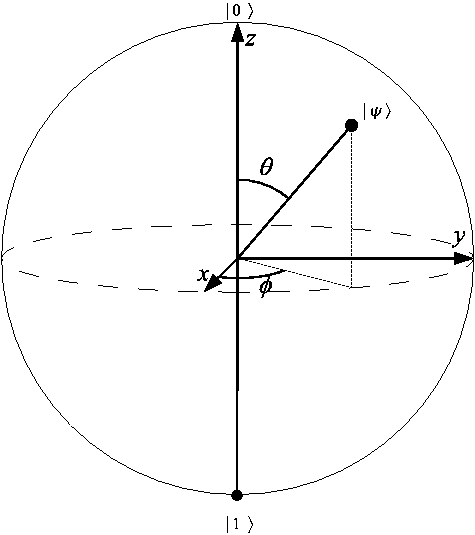
\includegraphics[scale=0.5]{Bloch.png}
\caption{The 1-Qubit Bloch Sphere \cite{QuantikiBlochSphereImage}}
\label{BlochSphere}
\end{figure}
A quantum state space can also been visualised in terms of the Bloch sphere, shown in Figure \ref{BlochSphere}.
The shown Bloch sphere is for a single qubit system, it can be extended to an n-qubit system however the visualisation breaks down.
All 'pure' quantum states can be described using the Bloch sphere and all exist on the surface produced by the unit sphere.
In this report only pure quantum states will be used and all explanation of quantum states are more precisely explanations of 'pure' quantum states.
This means that all superpositions of states can be expressed in terms of $|\psi\rangle = \cos \frac{\theta}{2} \, |0 \rangle +  e^{i \phi}  \sin \frac{\theta}{2}  \,|1 \rangle $ with $0 \leq \theta \leq \pi, \quad  0 \leq \phi \leq 2 \pi$, ignoring global phase factors\cite{BlochSphereTalk}.

In quantum mechanics, Kets are used to indicate a state, for example $\vert$0$\rangle$ is the state of a logical $0$ whereas $\vert$1$\rangle$ is the state of logical $1$.
Using this notation and the inclusion of probabilities, the state of the superposition can be expressed.

A dual to the Ket notation is the 'Bra' notation, $\langle$a$\vert$.
This notation is used to denote the 'dual vector' of the corresponding Ket.
For a state vector represented by
\begin{equation}\label{ket_explanation_example}
\vert
a
\rangle = 
\begin{pmatrix}
a_1\\
a_2\\
a_3\\
\vdots
\end{pmatrix}
\end{equation}
there is a dual vector representing its Hermitian conjugate
\begin{equation}\label{bra_explanation_example}
\langle
a
\vert = 
\begin{pmatrix}
a_1^*$$
a_2^*$$
a_3^*$$
\cdots
\end{pmatrix}
\end{equation}

Combining the two vectors $\langle$a$\vert$ and $\vert$b$\rangle$, written $\langle$a$\vert\vert$b$\rangle$, represents the inner product of the two vectors.
If a and b are unit vectors and $a == b$, $\langle$a$\vert\vert$b$\rangle == 1$.
If a and b are orthogonal, $\langle$a$\vert\vert$b$\rangle == 0$.

The outer product of two vectors, a and b, can be represented by $\vert$a$\rangle$$\langle$b$\vert$.
This represents the transformation from a to b.
It can also be represented in matrix form.

With
$\vert
0
\rangle
== 
\begin {pmatrix}
1\\
0\\
\end{pmatrix}
$
and
$\vert
1
\rangle
==  
\begin {pmatrix}
0\\
1\\
\end{pmatrix}
$
it is possible to represent $1$-qubit operations in the bra-ket notation.
For example, the NOT gate performs a simple negation of a qubit's value.
This can be written as $\vert0\rangle\langle1\vert + \vert1\rangle\langle0\vert$.
Substituting in the vector values we have
\begin{equation}
\begin{tabular}{ r c l }
\(\begin {pmatrix}
1\\
0
\end{pmatrix}
\begin {pmatrix}
0&&
1
\end{pmatrix}
 + 
\begin {pmatrix}
0\\
1
\end{pmatrix}
\begin {pmatrix}
1&&
0
\end{pmatrix}\)
& \(=\)
& \( 
\begin{pmatrix}
0 && 1 \\
0 && 0
\end{pmatrix}
 + 
\begin{pmatrix}
0 && 0\\
1 && 0
\end{pmatrix}
\) \\
& \(=\)
& \( 
\begin{pmatrix}
0 && 1 \\
1 && 0
\end{pmatrix}
\)
\end{tabular}
\label{eq:notexplanded}
\end{equation}

This matrix can be seen as a transformation matrix for the NOT operation.
In quantum computation, the NOT gate is one of the $4$ gates known as the Pauli gates, more specifically the Pauli-X gate.
It is called the Pauli-X gate as it can be seen as a rotation of $\pi$ radians about the X axis of the Bloch sphere, Figure \ref{BlochSphere}.

% Definition of Unitary
The matrices representing the Pauli-X gate and all other quantum logic gates are unitary.
A unitary matrix, U, is one which adheres to
\begin{equation}
U*{\dagger}
U == UU*{\dagger} = I_N
\end{equation}
where $I_N$ is the identity matrix in N dimensions and $U*{\dagger}$ is the complex conjugate of $U$.
% Reversible logic
The implication of all quantum logic operations being unitary is that they are reversible, this is a difference to classical computation.
With many classical logic gates irreversible, there is not a set of quantum logic gates which is as computationally powerful as the set of classical logic gates.
This seems like a major issue, quite the contrary.
The set of classical logic gates can be replaced by reversible equivalents and therefore it is possible to produce a set of quantum logic gates with the equivalent computational power as the classical logic gates.

%Superposition
As with all probabilities, the overall probability of a superposition collapsing to any of the states it contains must equal $1$.
\begin{equation}
\label{superposition_explanaiton}
\alpha\vert0\rangle+\beta\vert1\rangle
\end{equation}
\begin{equation}
\label{superposition_explanaiton_sum}
\frac{1}{2^{\frac{1}{n}}}\sum\limits_{i=0}^N \ket{x_i}
\end{equation}
Equation \eqref{superposition_explanaiton} is how the combination of the logical $0$ and $1$ states in a superposition can be represented for a single particle.
It can also be represented in the for of Equation \eqref{superposition_explanaiton}.
This is equivalent to the representation provided by the Bloch sphere, Figure \ref{BlochSphere}.
The probability of this state collapsing to the basis state $0$ can be calculated by $\vert\alpha\vert^2$ where $\alpha$ is a complex number.
$\alpha$ is known as the probability amplitude of $\vert0\rangle$.
Similarly, the probability of this state collapsing to the basis state $1$ can be calculated by $\vert\beta\vert^2$, $\beta$ being the probability amplitude of $\vert1\rangle$.
It follows that $\frac{1}{\sqrt{2}}\vert0\rangle+\frac{1}{\sqrt{2}}\vert1\rangle$ is an equal superposition where the collapse to 0 is just as likely as collapsing to $1$.
This provides the first glimpse of where a single qubit has the ability to perform a function not currently possible on a classical computer.
With n-qubits in the equal superposition, we have n binary values which have an equal probability of taking the value $0$ as the value $1$.
With an ordering decided of these qubits, collapsing the superposition of each qubit will result in a binary value of length n.
With all probabilities being $\frac{1}{2}$ this binary value takes a truly random value between $0$ and $2^n-1$.
It is not possible to produce a truly random number using a classical computer.

A second indication of the power held within the idea of superposition becomes clear if we look at the n-qubits in their equal superposition.
In 1935, Erwin Schr$\ddot{o}$ginger\cite{SchroedingersCat} proposed a thought experiment to explain the idea of superposition.
Imagine a cat in a fully opaque box with a vile of poison.
The vile may break at any time, a truly random variable.
After sealing the box the state of the cat is not known.
The cat could be alive if the vile has not broken but could just as likely be dead.
Only by looking inside the box will the state of the cat be known.
Until this time the cat could be thought of as both alive and dead at the same time.
If we assign 'dead' to the state $\vert0\rangle$ and 'alive' to the state $\vert1\rangle$ the situation looks very similar to the state we have previously seen.
Therefore, just as the cat can be thought of as both dead and alive at the same time, a qubit in the superposition $\frac{1}{\sqrt{2}}\vert0\rangle+\frac{1}{\sqrt{2}}\vert1\rangle$ can be thought of as both 0 and 1 at the same time.
This leads to a very powerful property of quantum computers.
With n classical bits, a single number in the range 0 to $2^n-1$ can be expressed at any one time.
With n quantum qubits, every number in the range 0 to $2^n-1$ can be expressed at any one time.
This effectively allows computation over the whole range of $2^n$ inputs to be carried out in parallel.

This parallelism is very powerful and has been shown to enable the computation of problems classified as NP to be performed in polynomial time.
This does however have a caveat.
As mentioned previously the superposition cannot itself be observed or measured.
When observed the superposition collapses to a basis state with respect to the superposition probability amplitudes.
This means that even though $2^n$ calculations can be performed in parallel, only a single answer can be observed.

% mathematic examples of matrices and the application
Along with the Pauli-X gate, there are an additional 3 Pauli gates.
The Pauli-I gate is the simplest of all quantum gates.
It is the identity gate, the output is identical to the input.
In Dirac notation this is $\vert0\rangle\langle0\vert + \vert1\rangle\langle1\vert$, and in matrix form below
\begin{equation}
\begin{tabular}{ r c l }
\(\begin {pmatrix}
1\\
0
\end{pmatrix}
\begin {pmatrix}
1&&
0
\end{pmatrix}
 + 
\begin {pmatrix}
0\\
1
\end{pmatrix}
\begin {pmatrix}
0&&
1
\end{pmatrix}\)
& \(=\)
& \( 
\begin{pmatrix}
1 && 0 \\
0 && 0
\end{pmatrix}
 + 
\begin{pmatrix}
0 && 0\\
0 && 1
\end{pmatrix}
\) \\
& \(=\)
& \( 
\begin{pmatrix}
1 && 0 \\
0 && 1
\end{pmatrix}
\)
\end{tabular}
\end{equation}

The Pauli-Z gate is similar to the Pauli-X gate, but differs in the axis about which it performs the rotation.
The Pauli-Z gate rotates the quantum state by $\pi$ radians about the Z axis.
This represents a phase flip of the quantum state.
The phase of a state is important when interference is used in computation.
In Dirac notation this is $\vert0\rangle
\langle0\vert + \vert1\rangle(-\langle1\vert$), and in matrix form below
\begin{equation}
\begin{tabular}{ r c l }
\(\begin {pmatrix}
1\\
0
\end{pmatrix}
\begin {pmatrix}
1&&
0
\end{pmatrix}
 + 
\begin {pmatrix}
0\\
1
\end{pmatrix}
\begin {pmatrix}
0&&
-1
\end{pmatrix}\)
& \(=\)
& \( 
\begin{pmatrix}
1 && 0 \\
0 && 0
\end{pmatrix}
 + 
\begin{pmatrix}
0 && 0\\
0 && -1
\end{pmatrix}
\) \\
& \(=\)
& \( 
\begin{pmatrix}
1 && 0 \\
0 && -1
\end{pmatrix}
\)
\end{tabular}
\end{equation}

The Pauli-Y gate is similar to both the Pauli-X and Pauli-Z gates, but differs in the axis about which it performs the rotation.
The Pauli-Y gate rotates the quantum state by $\pi$ radians about the Y axis.
This represents a phase flip followed by a bit flip.
In Dirac notation this is $\vert0\rangle
(i\langle1\vert) + \vert1\rangle(-i\langle0\vert$), and in matrix form below
\begin{equation}
\begin{tabular}{ r c l }
\(\begin {pmatrix}
1 \\
0
\end{pmatrix}
\begin {pmatrix}
0 &&
-i
\end{pmatrix}
 + 
\begin {pmatrix}
0 \\
1
\end{pmatrix}
\begin {pmatrix}
i &&
0
\end{pmatrix}\)
& \(=\)
& \( 
\begin{pmatrix}
0 && -i \\
0 && 0
\end{pmatrix}
 + 
\begin{pmatrix}
0 && 0\\
i && 0
\end{pmatrix}
\) \\
& \(=\)
& \( 
\begin{pmatrix}
0 && -i \\
i && 0
\end{pmatrix}
\)
\end{tabular}
\end{equation}

Along with the single qubit operations, like those above, there are operations which can act over n-qubits.
A simple example of a 2 qubit operation is the controlled-NOT, CNOT, operator.
This is a simple extension of the Pauli-X gate.
\begin{table}
\centering
\begin{tabular}{ l | c || r | }
0 & 0 & 0 \\
0 & 1 & 1 \\
1 & 0 & 1 \\
1 & 1 & 0 \\ \end{tabular}
\caption{Classical CNOT Truth Table}
\label{CNOTTruthTable}
\end{table}
The CNOT gate has a control input which it requires to be in the logical $1$ state for the NOT operation on the second input to be carried out.
In classical logic this would extend the truth table to be as shown in Table \ref{CNOTTruthTable}.
The truth table of the CNOT gate is the same as that of the XOR gate.
The Dirac notation of the CNOT gate is $\vert00\rangle\langle00\vert + \vert01\rangle\langle01\vert + \vert10\rangle\langle11\vert + \vert11\rangle\langle10\vert$.

\section{An Introduction to Quantum Algorithms}
%Known Quantum Algorithms

Just as with classical computers, the computation to produce the required output given inputs is given in the form of an algorithm.
Quantum algorithms can be constructed in several ways. These definitions are based on those provided by Massey\cite{masseythesis}.

\begin{itemize}
\item A quantum circuit can be used to represent an algorithm at the level of quantum logic gates.
This is similar to a specific purpose circuit diagram for classical systems.
\item A quantum program is a representation of the algorithm in some higher level quantum 'programming' language which would generate the required circuit.
The circuit generated is not defined in this method, just it's behaviour.
This could be seen as slightly more flexible that the quantum circuit model as the 'compiler' can be updated to reflect the findings of future research.
\item A parameterisable quantum algorithm is a representation in pure Pseudo-code.
It proves the flexibility of changing some value n, which is used to indicate the number of input qubits, to produce quantum circuits or programs with the desired behaviour on n qubits.
This is the most flexible construction of quantum algorithms.
It can cope with the changing in input size and can use findings of research just like in the 'compilation' of a quantum program.
\end{itemize}

Currently there are very few quantum algorithms known.
Peter Shor has carried out, and published, a discussion on the progress made `in discovering algorithms for computation on a quantum computer`\cite{Shor:2004:PQA:1032132.1032149}.
Shor suggests two possible reasons for the lack of quantum algorithms.
The first is `that there might really be only a few problems for which quantum computers can offer a substantial speed-up over classical computers`\cite{Shor:2004:PQA:1032132.1032149}.
This would indeed make the discovery of useful quantum algorithms difficult.
However, I feel this is somewhat pessimistic.
The main focus of the paper published by Feynman\cite{Feynman82simulatingphysics} was the problem of simulating the physics of quantum mechanics on a classical computer.
This to suggests there would be the potential of many applications of quantum computers, even if they aren't analogous to the classical computational applications.

The second is `that quantum computers operate in a manner so non-intuitive, and so different from classical computers`\cite{Shor:2004:PQA:1032132.1032149} that our current algorithm knowledge is close to useless.
This, in my opinion, is a much more believable obstacle.
Quantum mechanics is seen by many as a confusing and mystical subject.
Even prize winning mathematician and physicist Roger Penrose is attributed to the remark `Quantum mechanics makes absolutely no sense`.
Statements like this and the atmosphere surrounding quantum mechanics makes the potential of its study more than some what daunting.
As computer scientists, the exposure to and therefore our understanding of quantum mechanics is limited, in general.
With this in mind it is, currently, unreasonable to expect the discovery of algorithms that exploit the finer details of this complex and subtle theory to become an everyday occurrence.

The following few sections outline a selection of the currently known quantum algorithms.

\subsection{Deutsch Algorithms}
\label{sec:DeutAlg}
The original Deutsch algorithm\cite{Deutsch1985} was proposed to solve the following problem:
\begin{quote}
Given a function $f:\{0,1\}\to\{0,1\}$, decide whether it is either a balanced, or constant function.
The function $f(x)$ is guaranteed to be either constant or balanced.
\end{quote}
The algorithm's major breakthrough was that it only required a single invocation of the function $f(x)$ to decide on which category it belonged.
This is compared to the best classical approach requiring $2$ invocations to the function.
This was the first algorithm that it was possible to compute the solution to a problem, provably, more efficiently than a classical computer by exploiting quantum mechanics.

\begin{figure}
\[
\Qcircuit @C=1.0em @R=.7em {
& \lstick{\ket{0}} & \gate{H} & \gate{\mathcal{F}} & \gate{H} & \measure{meas} \\
& \lstick{\ket{1}} & \gate{H} & \targ\qwx & \rstick{\ket{0}-\ket{1}}\qw  
}
\]
\caption{Deutsch Circuit}
 \label{Deutsch-Cir}
\end{figure}

The circuit for this algorithm is presented in Figure \ref{Deutsch-Cir}.
The maths for the way in which the state evolves is below
\begin{equation}
\ket{01} \xrightarrow{H\otimes{H}} \frac{1}{\sqrt{2}}(\ket{0}+\ket{1})\frac{1}{\sqrt{2}}(\ket{0}-\ket{1})
\end{equation}

 Using the identity $(\ket{b}-\ket{a})\equiv-1(\ket{a}-\ket{b})$, if $f(x)$ evalues to $0$ the state transformation is
\begin{equation*}
 \ket{x}\frac{1}{\sqrt{2}}(\ket{0}-\ket{1}) \xrightarrow{f} \ket{x}\frac{1}{\sqrt{2}}(\ket{0}-\ket{1})
\end{equation*}
Wheras if $f(x)$ evaluates to $1$ the state transformation is
\begin{equation*}
 \ket{x}\frac{1}{\sqrt{2}}(\ket{0}-\ket{1}) \xrightarrow{f} -\ket{x}\frac{1}{\sqrt{2}}(\ket{0}-\ket{1})
\end{equation*}
These two equations can be generalised to give
\begin{equation*}
 \ket{x}\frac{1}{\sqrt{2}}(\ket{0}-\ket{1}) \xrightarrow{f} (-1)^{f(x)}\ket{x}\frac{1}{\sqrt{2}}(\ket{0}-\ket{1})
\end{equation*}
This is due to $(-1)^0=1$ and $(-1)^1=-1$ which is the way the state evolves with the outputs of $f(x)$.
Using this we can continue to analyse how the state evolves for the superposition $\frac{1}{\sqrt{2}}(\ket{0}+\ket{1})\frac{1}{\sqrt{2}}(\ket{0}-\ket{1})$.
\begin{equation*}
 \frac{1}{\sqrt{2}}(\ket{0}+\ket{1})\frac{1}{\sqrt{2}}(\ket{0}-\ket{1}) \xrightarrow{f} \frac{1}{\sqrt{2}}((-1)^{f(0)}\ket{0}+(-1)^{f(1)}\ket{1})\frac{1}{\sqrt{2}}(\ket{0}-\ket{1})
\end{equation*}
\begin{equation*}
 \frac{1}{\sqrt{2}}((-1)^{f(0)}\ket{0}+(-1)^{f(1)}\ket{1})\frac{1}{\sqrt{2}}(\ket{0}-\ket{1}) \equiv (-1)^{f(0)}\frac{1}{\sqrt{2}}(\ket{0}+(-1)^{f(0)\oplus{f(1)}}\ket{1})\frac{1}{\sqrt{2}}(\ket{0}-\ket{1})
\end{equation*}
This penultimate state, before the last hadamard, can be simplified.
Global phase factors cannot be observed so the $(-1)^{f(0)}$ can be ignored.
The second qubit can also be ignored as it is not entangled with the first, nor is it ever measured.
\begin{equation}
 \frac{1}{\sqrt{2}}(\ket{0}+(-1)^{f(0)\oplus{f(1)}}\ket{1})
\label{Deutsch_final_state}
\end{equation}
This results in the penultimate state being able to be represented as \ref{Deutsch_final_state}.
With this as the state we can reason about the output if the function $f(x)$ is balanced and if it is constant.
If f were balanced, $f(0) \oplus f(1) = 1$ due to either $f(0)$ or $f(1)$ evaluating to $1$ but not both.
If f were constant, $f(0) \oplus f(1) = 0$ due to either $f(0)$ and $f(1)$ both evaluating to $0$ or both evaluating to $1$.
Using these two observations we can see the penultimate state, \ref{Deutsch_final_state}, when f is constant and when f is balanced.
When f is balanced $\frac{1}{\sqrt{2}}(\ket{0}+(-1)^{f(0)\oplus{f(1)}}\ket{1}) \equiv \frac{1}{\sqrt{2}}(\ket{0}-\ket{1})$.
When this is passed through the final hadamard $\frac{1}{\sqrt{2}}(\ket{0}-\ket{1}) \xrightarrow{H} \ket{1}$.
When f is constant $\frac{1}{\sqrt{2}}(\ket{0}+(-1)^{f(0)\oplus{f(1)}}\ket{1}) \equiv \frac{1}{\sqrt{2}}(\ket{0}+\ket{1})$.
However, when this is passed through the final hadamard $\frac{1}{\sqrt{2}}(\ket{0}+\ket{1}) \xrightarrow{H} \ket{0}$.
This means that using just a single query to the function $f(x)$, the algorithm can provide an answer to the problem.


\subsection{Deutsch-Jozsa Algorithm}
%Deutsch-Jozsa Algorithm
The Deutsch-Jozsa algorithm\cite{1992-deutsch} is a generalisation and improvement over an earlier Deutsch algorithm\cite{Deutsch1985}.
The algorithm described here will be the algorithm including the improvements published in \cite{Macchiavello97quantumalgorithms}, the resulting algorithm is still referred to as the Deutsch-Jozsa algorithm.

In 1992, David Deutsch and Richard Jozsa\cite{1992-deutsch} presented an extension to the Deutsch algorithm, Section \ref{sec:DeutAlg}, that allowed for functions $f:\{0,1\}^{2n}\to\{0,1\}$ to be categorised as constant or balanced.
The algorithm was probabilistic but also required 2 invocations to the function $f(x)$.
This means that in the worst case, with $f_1:\{0,1\}\to\{0,1\}$, the algorithm will perform worst than both the original Deutsch algorithm\cite{Deutsch1985} and the classical algorithm due to the probabilistic nature of its result.
This is a very limited case and performance improves as the value of n increases.
As with the original algorithm, the number of invocations of $f(x)$ is constant, truly independent of both $n$ and $f(x)$.
This is again an improvement over the classical algorithm which requires in the worst case $2^{n-1}+1$ to be certain of the function's classification.
\begin{figure}
\[
\Qcircuit @C=1.0em @R=.7em {
& \lstick{\ket{0}} & \gate{H} & \multigate{3}{\mathcal{F}} & \gate{H} & \measure{meas} \\
& \lstick{\ket{0}} & \gate{H} & \ghost{\mathcal{F}} & \gate{H} & \measure{meas} \\
& \lstick{\ket{0}} & \gate{H} & \ghost{\mathcal{F}} & \gate{H} & \measure{meas} \\
& \lstick{\ket{0}} & \gate{H} & \ghost{\mathcal{F}}  & \gate{H} & \measure{meas} \\
& \lstick{\ket{1}} & \gate{H} & \targ\qwx & \rstick{\ket{0}-\ket{1}}\qw   
}
\]
\caption{Deutsch-Jozsa Circuit}
 \label{Deutsch-Jozsa-Cir}
\end{figure}

The algorithm requires n input qubits and a single control qubit.
The n input qubits are initialised to $\ket{0}$.
The control qubit is initialised to $\ket{1}$.
The n-fold Hadamard gates are then used to produce the superposition of all $0..2^n-1$ possible inputs, $x=(\ket{0}+\ket{1})^n$.
The Hadamard gate on the control qubit is used to produce the superposition $\ket{0}-\ket{1}$.
The difference in superpositions between the input and control qubits is important to the way in which the algorithm classifies a function.
This produces a state  $(\ket{0}+\ket{1})^n(\ket{0}-\ket{1})$.

% The n input qubits, in the superposition $(\ket{0}+\ket{1})^n$, are then passed to the function we wish to classify, $f(x)$.
The result of $f(x)$ is used as the control for a CNOT gate acting on the control qubit.
Remember at this point that the input x is in effect all possible inputs to $f(x)$, and as such the output is all the respective outputs.
This means that each of the factors of the input are transformed, based on the action of $f(x)$.
This can be formalised as $U_f(\ket{x},\ket{y})=(\ket{x},\ket{f(x)\oplus{y}})$.
Using the final Hadamard gates we can use the transformation to categorise $f(x)$.

If we assume n to be equal to 2, then after the initial Hadamard gates we have the superposition:
\begin{equation*}
\frac{1}{2}\ket{\Psi_{init}}\frac{1}{\sqrt{2}}(\ket{0}-\ket{1})=\frac{1}{2}(\ket{00}+\ket{01}+\ket{10}+\ket{11})\frac{1}{\sqrt{2}}(\ket{0}-\ket{1})
\end{equation*}
\begin{equation}
\ket{a}(\ket{c}-\ket{b})\equiv\ket{a}(-1(\ket{b}-\ket{c}))\equiv-1\ket{a}(\ket{b}-\ket{c})
\label{target_qubit_identity}
\end{equation}
The CNOT on the target qubit is only activated if $f(x)=1$ which, using the equivalent above, produces the superposition $-1(\ket{0}-\ket{1})$.
This can also be generalised as $(-1)^{f(x)}(\ket{0}-\ket{1})$ where $-1^1=-1$ and $-1^0=1$ by definition.
By linearity the superposition after the CNOT controlled by f(x) on the target qubit becomes
\begin{equation*}
\frac{1}{2}((-1)^{f(00)}\ket{00}+(-1)^{f(01)}\ket{01}+(-1)^{f(10)}\ket{10}+(-1)^{f(11)}\ket{11})\frac{1}{\sqrt{2}}(\ket{0}-\ket{1})
\end{equation*}

After the application of $f(x)$, the target bit has served it purpose and is neither measured nor entangled with any of the qubits from the n qubit input.
To simplify the equations I will now ignore the $(\frac{1}{\sqrt{2}}\ket{0}-\ket{1})$ contributed by the target qubit, the remaining state will be refereed to as $\Psi$.
If the function $f(x)$ is constant:
\begin{equation*}
\ket{\Psi_{const}}=\pm\frac{1}{2}(\ket{00}+\ket{01}+\ket{10}+\ket{11})
\end{equation*}
Whereas if $f(x)$ is balanced then:
\begin{equation*}
\ket{\Psi_{bal}}=(-1)^{f(00)}\ket{00}+(-1)^{f(01)}\ket{01}+(-1)^{f(10)}\ket{10}+(-1)^{f(11)}\ket{11}
\end{equation*}
However,as $\ket{\Psi_{const}}$ and $\ket{\Psi_{bal}}$ are orthogonal we can use this to detect if the function is balanced or constant.
\begin{equation*}
\bra{\Psi_{bal}}\ket{\Psi_{const}} = 0
\end{equation*}

Applying the n Hadamard gates to the state $\Psi_{const}$ produces the state $\pm\ket{0}^n$.
When measured this will return the result $0$ as the global phase factor $\pm$ cannot be observed.
As we have noted, $\Psi_{const}$ is orthogonal to $\Psi_{bal}$ so when the n Hadamard gates are applied, as they preserve orthogonality, the measured result will be anything orthogonal to $0$.
This gives us a clear way of distinguishing between whether f is constant of balanced with certainty and only a single invocation of f.
If the measurement returns $0$ then $f(x)$ is constant, if the measurement returns anything else $f(x)$ is balanced.

\subsection{Grover's Search Algorithm}	
%Grovers Database search algorithm
The Grover Search algorithm\cite{Grover:1996rk} is an unstructured search problem.
The algorithm assumes no underlying structure in the search space.
By this I mean the algorithm does not exploit, and therefore assume, any structure, such as sorting, in the data set being searched.

It has previously been proven\cite{Bennett:1996iu} that the lower complexity limit for any algorithm identifying an element without knowledge of underlying structure in the data is $\Omega(\sqrt{N})$.
For simplicities sake we assume $N=2^n$.
The complexity is measured by the number of elements which need to be queried in order to find the desired element.
The Grover Search algorithm has the complexity $O(\sqrt{N})$ and so `is within a constant factor of the fastest possible quantum mechanical algorithm`\cite{Grover:1996rk}.

\begin{figure}
\[
\Qcircuit @C=1.0em @R=.7em {
& \qw 		& \qw 	& \multigate{3}{f} 	&\qw 	&  \gate{H} 	&\qw 	& \multigate{3}{f_0} 	&\qw &  \gate{H}  	&\qw 	&\qw\\
& \vdots 	& 	&  \ghost{f} 		& \qw 	& \vdots 	& 	& \ghost{f_0} 		&\qw &  \vdots 		& 	&\qw\\
& \vdots 	& 	& \ghost{f} 		& \qw 	& \vdots 	& 	& \ghost{f_0} 		&\qw &  \vdots 		& 	&\qw\\
& \qw 		&\qw 	&  \ghost{f} 		& \qw 	& \gate{H} 	&\qw 	& \ghost{f_0} 		&\qw &  \gate{H} 	&\qw 	&\qw\\
& \qw 		&\qw 	&  \targ \qwx 		&\qw 	&  \qw 		&\qw 	& \targ \qwx 		&\qw &  \gate{X} 	&\qw	&\qw 
}
\]
\caption{Grover's Search Circuit}
 \label{Grovers-Search-Cir}
\end{figure}


The mechanisms used within the algorithm to produce a solution to the problem is more subtle than those used but the Deutsch-Jozsa algorithm.
The algorithm does not perform the computation in a single step.
The algorithm requires $O(\sqrt{N})$ steps.
The section of circuit which is repeated is that shown in Figure \ref{Grovers-Search-Cir}.

The algorithm is to initialise the state, $\Psi_1$, using n Hadamard gates.
\begin{equation*}
\Psi_1=\frac{1}{2^{\frac{1}{n}}}\sum\limits_{i=0}^N \ket{x_i}(\ket{0}-\ket{1})
\end{equation*}
The application of $f(x)$ is used in an analogous way to in the Deutsch-Jozsa algorithm.
It can again be written as $U_f(\ket{x},\ket{y})=(\ket{x},\ket{f(x)\oplus{y}})$ and remember
\begin{equation*}
 \exists{x_i}\epsilon\{x_0,x_1,\ldots,x_{n-1}\}|f(x_i)=1
\end{equation*}
\begin{equation*}
\forall{x_j} : i\neq{j} : f(x_j)=0
\end{equation*}
Just as in the Deutsch-Jozsa algorithm, the result of a $1$ produces a bit flip on the target qubit.
Using the identity in Equation \ref{target_qubit_identity} this flips the sign on the amplitude associated with $x_i$, where $f(x_i)=1$.
The state $\Psi_1$ is transformed by $U_f$ to $\Psi_2$.
\begin{equation*}
\Psi_2=\frac{1}{2^{\frac{1}{n}}}\sum\limits_{j=0\wedge{j}\neq{i}}^N \ket{x_j}(\ket{0}-\ket{1}) - \frac{1}{2^{\frac{1}{n}}} \ket{x_i}(\ket{0}-\ket{1})
\end{equation*}
The second function in the circuit, $f_0(x)$, is a fixed function.
It is not dependant on $f(x)$ but is a function which evaluates to $1$ only when the input is $\ket{0}$.
This means that given a simple state $(\alpha\ket{0}+\beta\ket{1}+\ldots)$ the result is the state $(-\alpha\ket{0}+\beta\ket{1}+\ldots)$.
The action of both these function can be written in the shorter and much simpler Dirac notation.
\begin{equation*}
U_f=I-2\ket{x_i}\bra{x_i}
\end{equation*}
\begin{equation}
U_0=I-2\ket{0}\bra{0}
\label{Grover:U_0_dirac}
\end{equation}

Functions $f(x)$ and $f_0(x)$ seem relatively unimpressive and don't appear to solve the problem.
The importance of the two sets of n Hadamard gates, one each side of $f_0(x)$, is paramount.
The effect they have on the action of $f_0(x)$ is shown below, the action of $f_0(x)$ and the Hadamard gates will be represented as V.
\begin{equation*}
V=H^{\otimes{n}}U_0{H}^{\otimes{n}}
\end{equation*}
\begin{equation*}
V=H^{\otimes{n}}(I_n-2\ket{0}\bra{0}){H}^{\otimes{n}}
\end{equation*}
\begin{equation*}
V=H^{\otimes{n}}I_n{H}^{\otimes{n}}-H^{\otimes{n}}(2\ket{0}\bra{0}){H}^{\otimes{n}}
\end{equation*}
\begin{equation*}
V=I_n-2(H^{\otimes{n}}\ket{0})(\bra{0}{H}^{\otimes{n}})
\end{equation*}
\begin{equation*}
V=I_n-2(H^{\otimes{n}}\ket{0})({H}^{\otimes{n}}\ket{0})^\dagger
\end{equation*}
The application of Hadamard gates to the $\ket{0}$ state is the method of creating the superposition of all $2^n-1$ possible states.
\begin{equation*}
V=I_n-2(\frac{1}{2^{\frac{1}{n}}}\sum\limits_{i=0}^N \ket{x_i})(\frac{1}{2^{\frac{1}{n}}}\sum\limits_{i=0}^N \ket{x_i})^\dagger
\end{equation*}
\begin{equation*}
V=I_n-2(\frac{1}{2^{\frac{1}{n}}}\sum\limits_{i=0}^N \ket{x_i})(\frac{1}{2^{\frac{1}{n}}}\sum\limits_{i=0}^N \bra{x_i})
\end{equation*}
\begin{equation*}
V=I_n-2\ket{\Psi}\bra{\Psi}
\end{equation*}
Just as with $U_f$, V can be seen as a simple phase flip.
However, the subtlety of this operator is that the flip is not in the computational basis, but in the basis described by $\ket{\Psi}$.

The last gate in Figure \ref{Grovers-Search-Cir} is the Pauli-X operator.
This is not functional but for convenience of mathematics as produces a global phase flip of $\ket{\Psi}$ which makes the mathematics simpler.

That is Grovers algorithm.
Looking at the circuit and the mathematics of the operators it doesn't provide an obvious answer as to how it solves the search problem.
This is partly due to the fact the circuit in Figure \ref{Grovers-Search-Cir} has to be repeated roughly $\frac{\pi\sqrt{N}}{4}$ times and partly due to the effect of the circuit being hidden in implementation.
The circuit is actually little more than a complex rotation gate.
It is however more sophisticated than a standard rotation gate as it computes the direction to rotate the state so as to solve the problem.
The power of this does not initially appear as immense as it possibly should.
The Hilbert space in which this circuit is operating is of the order $N$, we as humans can only accurately imagine a maximum of a $3$ dimensional space as it the most dimensions we can observe directly.
Taking into account the vast Hilbert space when assessing this circuit produces a much better appreciation its power.

However, even though the power can now be appreciated, the way in which it solves the problem is still not clear. 

\subsection{Shor's Factorisation Algorithm}
%Shors Algorithm
In 1994, Peter Shor astonished the computer science community with a quantum factorisation algorithm\cite{Shor:1994jg}.
This allowed the factorisation of integers into their constituent primes in polynomial time.
This algorithm is not a pure quantum algorithm, but a hybrid algorithm.
It has both a quantum and classical portion.

The algorithm utilises the complex nature of the probability amplitudes.
This means that the relative phase of the states is important.
To explain Shors algorithm it is necessary to introduce the sum of complex roots of unity.

\begin{equation}
 \sum_{j=0}^{N-1}z^j=\frac{1-z^N}{1-z}
\label{sumofpowers}
\end{equation}

Equation \ref{sumofpowers} provides a simplification of the sum of the geometric series $\sum_{j=0}^{N-1}z^j$.
This simplification can be applied to both real and complex values of z, including the roots of unity.
Taking $w=e^{\frac{2\pi{i}}{N}}$ to be the N-th root of unity, the geometric series $\sum_{i=0}^{N-1}w^{xy}$ can be simplified using Equation \ref{sumofpowers}.

When $x=0$
\begin{equation}
 \sum_{y=0}^{N-1}w^{xy}=\sum_{y=0}^{N-1}w^{0}=\sum_{y=0}^{N-1}1 = N
\end{equation}
However, when $x\neq{0}$
\begin{equation}
 \sum_{y=0}^{N-1}w^{xy}=\sum_{y=0}^{N-1}(w^x)^y=(\frac{1-w^N}{1-w})^y=0^y=0
\end{equation}
The result of this is generally described using a Kronecker delta
\begin{equation}
 \sum_{y=0}^{N-1}w^{xy}=N\times\delta_{x,y}=N\times
\left\{
  \begin{array}{cc} 1, & \mbox{if } x={0}\\ 
  0, & \mbox{if } x\neq{0}\end{array}
\right.
\label{krondelt}
\end{equation}

This produces a very neat and convenient explanation of such a series.
As the sum is of a root of unity raised to a power, it is a periodic function $w^0=w^N=1$.
This holds true in Equation \ref{krondelt} when $x=0,\pm{N},\pm{2N},\dots$.
With this the Kronecker delta can be expressed in terms of modular arithmetic.
\begin{equation}
 \sum_{y=0}^{N-1}e^{\frac{2\pi{i}xy}{N}}=N\times\delta_{x,y (mod N)}=N\times
\left\{
  \begin{array}{cc} 1, & \mbox{if } x={0}\\ 
  0, & \mbox{if } x\neq{0}\end{array}
\right.
\label{krondelt}
\end{equation}

The quantum section of Shor's algorithm is a period finding function.
The classical part then uses this period and number theory to deduce the factors.
In the explaination below, the value that is trying to be factorised is $N$ and the value $M$ is a value which is larger than $N$.
The use of the Kronecker delta, and understanding on the effect it has is vital to the explanation of the quantum section of Shor's algorithm.

\begin{figure}
\[
\Qcircuit @C=1.0em @R=.7em {
&\ket{0}&	& \qw	&\multigate{3}{\mathcal{F}^{-1}_M}	& \qw 	&\multigate{3}{f}	&\qw &\multigate{3}{\mathcal{F}_M}	&\qw	& \qw 	& \qw 	&\qw\\
&\vdots	&	&	&\ghost{\mathcal{F}^{-1}_M} 		&\qw 	&\ghost{f}		&\qw &\ghost{\mathcal{F}_M}		&	&\vdots & 	&\qw\\
&\vdots	&	&	&\ghost{\mathcal{F}^{-1}_M} 		&\qw 	&\ghost{f}		&\qw &\ghost{\mathcal{F}_M}		&	&\vdots & 	&\qw\\
&\ket{0}&	&\qw	&\ghost{\mathcal{F}^{-1}_M} 		&\qw 	&\ghost{f}		&\qw &\ghost{\mathcal{F}_M}		&\qw	&\qw 	&\qw	&\qw\\
&\ket{0}&	&\qw	&\qw 					&\qw 	&\multigate{3}{+}\qwx	&\qw &\qw 				&\qw	&\qw 	&\qw	&\qw\\
&\vdots	&	&	&\vdots 				&	&\ghost{+}		&\qw &\vdots 				&	&\vdots	&	&\\
&\vdots	&	&	&\vdots 				&	&\ghost{+}		&\qw &\vdots 				&	&\vdots	&	&\\
&\ket{0}&	&\qw	&\qw 					&\qw	&\ghost{+}		&\qw &\qw 				&\qw	&\qw	&\qw 	&\qw    
}
\]
\label{shorcirc}
\caption{The circuit of Shor's algorithm}
\end{figure}

The circuit in Figure \ref{shorcirc} is the period finding section of Shor's Algorithm.
The function $f$ is a periodic function, whose period we want to find.
$\mathcal{F}$ and $\mathcal{F}^{-1}$ are the Quantum Fourier Transform and the inverse, respectively.
\begin{equation}
 \mathcal{F}_N\ket{x}=\frac{1}{\sqrt{N}}\sum_{y=0}^{N-1}e^{\frac{2\pi{i}xy}{N}}\ket{y}
\label{QFTeq}
\end{equation}
\begin{equation}
 \mathcal{F}^{-1}_N\ket{y}=\frac{1}{\sqrt{N}}\sum_{z=0}^{N-1}e^{\frac{-2\pi{i}xy}{N}}\ket{z}
\label{QFTInveq}
\end{equation}

The action of applying the Quantum Fourier Transform and the inverse can be seen in Equations \ref{QFTeq} and \ref{QFTInveq} respectively.

The way in which this circuit computes the period is not initially apparent.
The central section of the circuit, involving the periodic function, performs the operation $U_f\ket{x}\ket{y}=\ket{x}\ket{f(x)+y}$ in the computaional basis.
However, it is preceded by the inverse Quantum Fourier Transform.
The application of the inverse Quantum Fourier Transform on the initial state is as follows:

\begin{equation*}
 \ket{0}\ket{0} \rightarrow \frac{1}{\sqrt{M}}\sum_{x=0}^{M-1}e^{\frac{-2\pi{i}x.0}{M}\ket{x}\ket{0}}
\end{equation*}
\begin{equation*}
 \frac{1}{\sqrt{M}}\sum_{x=0}^{M-1}\ket{x}\ket{0}
\end{equation*}

This produces a uniform superposition, just as a series of Hadamard gates would have produced.
The application of $f(x)$ to this superposition produces the state:
\begin{equation*}
 \frac{1}{\sqrt{M}}\sum_{x=0}^{M-1}\ket{x}\ket{f(x)}
\end{equation*}
Applying the final Quantum Fourier Transform manipulates this state quite substantially.
\begin{equation}
 \frac{1}{\sqrt{M}}\sum_{x=0}^{M-1}\ket{x}\ket{f(x)} \rightarrow \frac{1}{M}\sum_{y=0}^{M-1}\sum_{x=0}^{M-1}e^{\frac{2\pi{i}xy}{M}}\ket{y}\ket{f(x)}
\label{QFTfinstate}
\end{equation}
The final state is Equation \ref{QFTfinstate}.
This does not initially appear particularly useful or interesting.
However, remembering that $f(x)$ is periodic, we can separate and analyse a single branch of the superposition.
With $f(x)=f(x+r)=f(x+2r)\dots$ where $r$ is the period of $f(x)$ the amplitude of the branch $\ket{y}\ket{f(x)}$ , with $x=x_0+mr for x=0,1,\dots,\frac{M}{r}-1$, can be written as:
\begin{equation*}
 \frac{1}{M}\sum_{m=0}^{\frac{M}{r}-1}e^{\frac{2\pi{i}(x_0+mr)y}{M}}\ket{y}\ket{f(x_0)}
\end{equation*}

This initially still does not look particularly interesting or useful when we are trying to find the period of $f(x)$.
However, with some rearragement this state can be expressed as:
\begin{equation}
 \frac{1}{M}e^{\frac{2\pi{i}x_0y}{M}}\sum_{m=0}^{\frac{M}{r}-1}e^{\frac{2\pi{i}my}{\frac{M}{r}}}\ket{y}\ket{f(x_0)}
\end{equation}
This contains a structure which was introduced with the sumation of roots of unity, \ref{sumofpowers}.
Using this observation, the $\sum_{m=0}^{\frac{M}{r}-1}e^{\frac{2\pi{i}my}{\frac{M}{r}}}$ section of the amplitude for the state $\ket{y}\ket{f(x_0)}$ is simplified to:
\begin{equation}
 \sum_{m=0}^{\frac{M}{r}-1}e^{\frac{2\pi{i}my}{\frac{M}{r}}}=\frac{M}{r}\delta_{y,0 (Mon\frac{M}{r})}=\frac{M}{r}
\left\{
  \begin{array}{cc} 1, & \mbox{if } y={0} (mod\frac{M}{r})\\ 
  0, & \mbox{otherwise}\end{array}
\right.
\end{equation}
With this simplifcation in place it can be seen that the probability amplitude of any branch where $y\neq{x}(mod\frac{M}{r})$ will be zero simply due to the Kronecker delta.
This results in the only branches with non-zero amplitudes being where $y=0,\frac{M}{r},\frac{2M}{r},\dots$ and so when the first input register is measured the state observed will be $\ket{\frac{kM}{r}}$.
After several repeats of the algorithm the value of $r$ can be deduced from the observed states.

To see how knowing the period can help factorise the number $N$ we analyse the function $f(x)=a^x(mod N)$.
This function is obviously periodic as it is modulo N.
With the period r, $a^r=1(mod N)$.
The value of $r$ will depend on the value of $a$.
Only the even values of $r$ are useful, if an odd value is found the value of $a$ should be changed and the new $r$ found.

When $r$ is even, $a^r=1(mod N) \rightarrow a^r-1=0(mod N) \rightarrow (a^r+1)(a^r-1)=0(mod N)$.
Once we have the equation in this form, we can use the values of $a^r+1)$ and $(a^r-1)$ separately as one of them, possibly both, with have a factor in common with $N$.
This can simply be found using the Chinese remainder theorm.

The advantage of Shor's algorithm is that the value of $r$ can be found much faster with all values of $x$ up to the limit of $M-1$ tested simultaneously.

\subsection{Quantum Teleportation Protocol}

The quantum teleportation protocol provides a solution to the problems
\begin{center}
Alice has a quantum state, $\ket{\Psi}$, which she wishes to send to Bob.
There is only a classical communication channel by which Alica and Bob can communicate.
\end{center}

With a classical state this would not be an issue.
Measurements on the different parts of that state Alice want to sent to Bob would be made, and these would then be communicated down the channel for Bob to replicate.
Unfortunately this is not possible for quantum states.
Quantum computation exploits the power of quantum mechanics, however quantum mechanics has its own caveats.

The ``No Cloning Theorm'' in the field of quantum computation is the results of quantum mechanic's ``Uncertainty Principle''.
The ``Uncertainty Principle'' states that ``that
the values of a pair of canonically conjugate observables such as position and momentum cannot both
be precisely determined in any quantum state''\cite{uncerth}.
Essentially this means that an unknown quantum state cannot be reproduced.

The classical approach is also halted by Holevo's Theorem.
This theorem states that from any $n$ qubit state, at most $n$ bits of classical information can be observed.
With a one qubit state, $\alpha\ket{0}+\beta\ket{1}$, the value of $\alpha$ and $\beta$ are required for the state to be reproduced.
The each of these require 2 values as they are complex numbers, 4 values in total.
The state can be rewriten to give $|\alpha|e^{i\theta_0}\ket{0}+|\beta|e^{i\theta_1}\ket{1}$.
As global phase factors cannot be observed it can be simplified to $|\alpha|\ket{0}+|\beta|e^{i\phi}\ket{1}$
This leaves the real values $|\alpha|, |\beta| and \psi$, down to 3 values.
We know that $|\alpha|^2+|\beta|^2=1$ so the value of $|beta|$ is can be calculated from the value of $|\alpha|$.
This leave just two values to specify.
However, both of these two values can be specified to any arbitary precision, requiring an arbitary number of bits of data.
As Holevo's Theorem limits the observable information to just a single bit, for the one qubit state, the measure and recreate approach is impossible.

After stating these two theorems, the problem Alice and Bob face seems impossible.
However, there are subtleties to the laws governing quantum mechanics which actually make it possible, with a few concessions.

For Alice to sent the state $\ket{Phi}$, $\alpha\ket{0}+\beta\ket{1}$, the protocol is as follows:
\begin{itemize}
 \item Alice and Bob share the entangled state $\frac{1}{\sqrt{2}}\ket{00}+\frac{1}{\sqrt{2}}\ket{11}$.
This results in the state, the subscript letters are to show who is in possession of which qubits:
\begin{equation}
 \frac{1}{\sqrt{2}}(\alpha\ket{00}_A\ket{0}_B+\beta\ket{10}_A\ket{0}_B+\alpha\ket{01}_A\ket{1}_B+beta\ket{11}_A\ket{1}_B)
\end{equation}
\item Alice takes a measurement in the Bell Basis.
The Bell basis is a basis set which are not orthogonal to the computational basis.
This means that the measurement does not collapse the state.
The Bell basis vectors are $\ket{00}+\ket{11}, \ket{00}-\ket{11}, \ket{01}+\ket{10} and \ket{01}-\ket{10}$.
\begin{center}
\begin{tabular}{cc}
Alice measures & Remaining state\\
$\ket{00}_A+\ket{11}_A$ & $\alpha\ket{0}_B+\beta\ket{1}$\\
$\ket{00}_A-\ket{11}_A$ & $\alpha\ket{0}_B-\beta\ket{1}_B$\\
$\ket{01}_A+\ket{10}_A$ & $\alpha\ket{1}_B+\beta\ket{0}_B$\\
$\ket{01}_A-\ket{10}_A$ & $\alpha\ket{1}_B-\beta\ket{0}_B$
\end{tabular}
\end{center}

\item Based on the measurement Alice make she can instruct Bob, using the classical communication channel, to perform certain operations to change the remaining state into the original state $\ket{\Psi}$.
\begin{center}
\begin{tabular}{cc}
Remaining state & Bob applies to produce $\ket{\Psi}$\\
$\alpha\ket{0}_B+\beta\ket{1}_B$ & Nothing\\
$\alpha\ket{0}_B-\beta\ket{1}_B$ & Phase Flip\\
$\alpha\ket{1}_B+\beta\ket{0}_B$ & Bit Flip\\
$\alpha\ket{1}_B-\beta\ket{0}_B$ & Bit Flip followed by a Phase Flip
\end{tabular}
\end{center}
\end{itemize}

At the end of this protocol, the state $\ket{\Psi}$ has be teleported to Bob.
However, this must not violate either the No Cloning Theorem or Holevo's Theorem.
The No Cloning Theorem is not violated as to teleport the state to Bob, Alice must destroy her copy of $\ket{\Psi}$.
This means that at no point are there two copies of $\ket{\Psi}$, therefore does not violate the No Cloning Theorm.
The protocol does not violate Holevo's Theorem as at no point is any data observed from the state.
The true identity and nature, the probability amplitues, of the state $\ket{\Psi}$ is never known.

The circuit to implement the quantum teleportation protocol can be seel in Figure \ref{quantelcir}.

\begin{figure}
\[
\Qcircuit @C=.7em @R=.4em @! {
\lstick{\ket{\psi}} & \qw & \qw & \ctrl{1} & \gate{H} & \meter & \control \cw\\
\lstick{\ket{0}} & \qw & \targ & \targ & \qw &\meter & \cwx\\
\lstick{\ket{0}} & \gate{H} & \ctrl{-1} & \qw &\qw & \gate{X} \cwx & \gate{Z} \cwx &\rstick{\ket{\psi}} \qw
}
\]
\label{quantelcir}
\caption{The Quantum Teleportation Circuit\cite{qcirtut}}
\end{figure}
% \section{The Current State of Quantum Computing}
% --Problems with current algorithms
% 
% 	--Scalability
% 	
% 	--Require many more Qubits than are available with current hardware implementations
% 
%  
% --Current State of QC
% 	
% 	--Latest hardware
% 	
% 	--Latest algorithms

\section{The Use of Evolutionary Computation in the Synthesis of Quantum Algorithms}
%Need to read a lot more
% different representations
% ways to simulate them
Nature inspired computation is a highly active research area.
Taking inspiration from nature and biological theories, search techniques such as Genetic Algorithms and Genetic Programming are being employed to a wide rage of industrial problems.
What makes these approaches different is that they are based on a population, or 'generation', of individuals.
The basic principle is to take an 'individual' of a defined representation, evaluate it's 'fitness' to perform the task required and to 'mutate' it randomly and add it to the next 'generation' of individuals.
Along with mutation, a computational analogy to biology's reproduction, called crossover, can be used.
Crossover takes two, or potentially more, individuals and combines them to produce other individuals which are then added to the next 'generation'.
The each cycle of evaluate, selection and mutation and/or crossover produces a 'generation' of individuals.
The process repeats until a required 'fitness' is found or a resource limit is reached, time or number of generations produced for example.
As the process progresses, with the a reasonable representation and fitness function, the average 'fitness' of each generation should improve.

The use of evolutionary techniques to try synthesize quantum algorithms is not new.
There are many examples of successes in producing solutions to problems already solved by a manual approach and some producing novel solutions to previously quantumly unsolved problems.
The techniques used vary from Genetic Algorithms to Genetic Programming with varying success.

Not only is the technique varied, the desired solution is also varied.
Some research focuses on the evolution of quantum circuits or programs, whereas some focus on more general quantum algorithms which take a parameter representing the number of input qubits.
Due to the exponential increase in resources required for simulation with an increase in qubits the generality of the quantum algorithms is not usually tested on large systems.

\subsection{Q-PACE I}
Massey\cite{masseythesis,masseymeng} explores both Genetic Algorithms and Genetic Programming as search techniques.
The software suites presented, Q-PACE I - IV, have varying success and increase in search power.
Q-PACE I\cite{masseymeng} is described as solving `a number of basic proof of concept problems`\cite{masseythesis} and `proves the concept that evolutionary search techniques can be used to evolve quantum software`\cite{masseythesis}.
Q-PACE I uses a fixed length array of quantum gates and is based on a simple Genetic Algorithm found in \cite{1989goldberg}.

Q-PACE II\cite{masseythesis} is a suite based on Q-PACE I but uses Genetic Programming instead.
In contrast to Q-PACE I, Q-PACE II is able to handle variable length solutions as individuals are represented as a list of quantum gates parameterized with the label, target and control bits and phase factor.
It also includes the inclusion of vector manipulation rather than matrix manipulation to improve efficiency.
Matrix manipulation is a simple concept, however it is very computationally expensive.
Operators are just one to one functions acting on state vectors.
\begin{equation}
 \begin{pmatrix}
\alpha_0\\
\alpha_1\\
\alpha_2\\
\alpha_3
\end{pmatrix}
\rightarrow
 \begin{pmatrix}
\alpha_2\\
\alpha_3\\
\alpha_0\\
\alpha_1
\end{pmatrix}
\label{vectormanipulation}
\end{equation}

The operation of the Pauli-X gate on the first qubit in a two qubit system can be represented as Equation \ref{vectormanipulation}.
For more complex gates, such as the Hadamard gate, the matrix manipulation is much more expensive than the equivalent vector manipulation.

\subsection{Q-PACE II}
The representation used in Q-PACE II is not able to express a Toffoli, Controlled-Controlled-Not, gate as a single gate.
This makes evolving a half-adder circuit more than a trivial test.
When Q-PACE II is tested against producing a circuit with the specification $\ket{x, y, z}\rightarrow\ket{x,x \oplus y, x \wedge y}$ it is able to produce several exact solutions.
One of which was claimed, at the time, to be the `best known solution to the problem`\cite{masseythesis} with the restricted gate set.
Q-PACE II was also challenged to produce a circuit to implement $\ket{c, a, b, z}\rightarrow\ket{c, a, (a+b)_0, (a+b)_1}$ and again produced `the most efficient solution to this particular problem`\cite{masseythesis}.

\begin{equation}
\begin{pmatrix}
a\\
b\\
0\\
0\\
0\\
0\\
0\\
0
\end{pmatrix}
\label{masseyprobref}
\end{equation}

Both tests of Q-PACE outlined were carried out to produce a deterministic solution, would always present the correct answer after measurement.
Further tests were performed on more complicated problems, however deterministic solutions were not found.
Following on from the work carried out by Spector et al\cite{LSpectorGPforQC,LSpectorANDOR,Spector:1999:QCA:316573.317112}, Massey changed to a probabilistic approach.
The definition, referring to \ref{masseyprobref}, of a probabilistic solution used by Massey is:

\begin{quote}
The probability of measuring $\ket{000}$ is at least $0.5 \times a\bar{a}$, and the probability of measuring $\ket{001}$ is at least $0.5 \times b\bar{b}$.\cite{masseythesis}
\end{quote}

With this new, relaxed, requirement of probabilistic correctness, the Q-PACE II software was used to `evolve a quantum circuit to implement the specification 
\begin{equation*}
 \ket{a_1, a_0, b_1, b_0, z_1, z_0} \rightarrow \ket{a_1, a_0, (a+b)_2, (a+b)_1, (a+b)_0, z_0}'
\end{equation*}
The result was, despite the requirement of only probabilistic correctness, a deterministic solution to the problem\cite{masseythesis}.
The evolved circuit was not as efficient by that presented in \cite{Vedral:1995ga} but was still deterministic.

\begin{figure}
\Tree [.Create\_CN [.Create\_N 1 ] [.Create\_H 2 ]]
\caption{Q-PACE III Example Solution Tree}
\label{QPACEIIIEXTREE}
\end{figure}

\begin{figure}
\[
\Qcircuit @C=1.0em @R=.7em {
& \qw & \gate{N} & \qw &  \ctrl{1} & \qw \\
& \qw & \qw & \gate{H} & \targ & \qw
}
\]
\caption{Q-PACE III Example Program Output}
\label{QPACEIIIEX}
\end{figure}


\subsection{Spector \emph{et al}, Deutsch's Problem}
Lee Spector \emph{et al}\cite{LSpectorGPforQC,LSpectorANDOR,Spector:1999:QCA:316573.317112} published a paper which used a different evolutionary approach.
They used Genetic Programming to produce a better than classical solution to the original Deutsch\cite{Deutsch1985} problem.
This was not an unsolved problem as explained in Section \ref{sec:DeutAlg}, however it was an example of where quantum computation was known to be more efficient than any possible classical approaches.

The genetic programming approach taken was the traditional tree based representation.
The level at which the solution was represented was higher than that of both Q-PACE I and Q-PACE II.
Both Q-PACE and Q-PACE II evolved quantum circuits whereas Spector represent solutions as ``classical programs which, when executed, construct quantum gate arrays''.
This is the quantum program representation as defined earlier.

The best solution produced a quantum gate array which did compute the answer to the Deutsch problem but was different to the Deutsch circuit\ref{Deutsch-Cir}.
However, it was still provably more efficient than any classical algorithm.

As well as fixed size solutions, the function set, non-terminal set for the Genetic Programming tree, included the control structures required to produce parameterisable quantum algorithms.
These were not used to attempt a solution to the Deutsch Jozsa problem, which would have seemed the more obvious progression, but the \emph{majority-on} problem.
The majority-on problem it to decide whether the output of a function has a majority of outputs being $1$.

The best solution was a parameterisable algorithm which, for functions with a large variation from $2^{n-1}$ of $1$'s the solution performed well.
However, when tested on functions with $2^{n-1}$ inputs evaluating to $1$ the solution ends up with an output error of $0.5$.

Both the solution for the Deutsch problem and the \emph{majority-on} problem were searched for with a probabilistic approach, looking for solutions with an output error of lower than 0.48 rather than for deterministic solutions.

\subsection{Q-PACE III}
Massey's third generation, Q-PACE III, evolved quantum programs, inspired by the Spector\cite{LSpectorGPforQC,LSpectorANDOR,Spector:1999:QCA:316573.317112} results and taking on one of the suggested ``Future Work'' topics.
Just as with Q-PACE II, Q-PACE III was a Genetic Programming suite.
The solutions evolved by Q-PACE III were executable programs, 'second order' solutions, which produce as an output a quantum circuit.
An additional difference between the two suites is the representation.
Q-PACE III represents programs as trees, rather than lists.
The execution of the solutions is performed by a pre-order traversal of the solutions tree representation.
The tree in \ref{QPACEIIIEXTREE} produces the circuit in \ref{QPACEIIIEX}.

Due to the change in representation, the evolutionary operations, mutation and crossover, occur at the second order level.
As shown in \ref{QPACEIIIEXTREE}, the different non-terminal nodes were of different arrity, allowing for more expressive trees.
Whereas in Q-PACE I and II the fitness of an individual could be calculated directly from the individual, in Q-PACE III the individuals have to be `executed` to produce the quantum circuit before the fitness can be evaluated.
With this additional step, the fitness evaluation requires more computational resources.

Massey defines the PF Max problem as
\begin{quote}
 You are given a permutation function f(x) which operates over the integer range [0..3].
Using a suitable encoding, evolve a quantum program U which returns the value of x that gives the maximum value of f(x).\cite{masseythesis}
\end{quote}
Q-PACE III was used to try find a probabilistic solution to the PF Max problem.
The experiment was successful.
When tested against the 8 permutations used as fitness cases, the correct result was the probabilistic result in each case.
When tested against the 24 possible permutations, the correct result was the probabilistic result in 20 of the 24 cases.

It was found that if the acceptance requirement was reduced to 0.4, from 0.5, a quantum program was evolved which returns the correct value for all 24 possible permutation exactly $50\%$ of the time.
This result was quite remarkable, this probability is twice that of the best classical approach, guessing.

\begin{equation}
 y_k = \frac{1}{\sqrt{N}} \sum_{j=0}^{N-1}{x_j}e^{\frac{2\pi{ijk}}{N}}
\label{QFTeqn}
\end{equation}

Q-PACE III was also used to evolve an solution which, when run, produced the circuit for the Quantum Fourier Transform on 3 qubits.
The Quantum Fourier Transform is an operation defined by equation \ref{QFTeqn} where x, $(x_0, x_1, \ldots, x_{N-1})$ where $N = 2^n$, is the input state and y, $(y_0, y_1, \ldots, y_{N-1})$, is the resulting state.
It is fundamental for Shor's factorisation algorithm.
The problem was approached both deterministically and probabilistically, both were successful.
The results of the probabilistic experiments were unexpected.
The definition of the acceptance requirement had to be generalised.
Whereas for the PF Max problem the correct answer was a single value, the correct answer for the Quantum Fourier Transform is a state vector.
An acceptance level of $x\%$ was redefined as the requirement that for all fitness cases, each state has a probability of being measured of at least $x\%$ of the probability for the respective state after running a `perfect` Quantum Fourier Transform.
It was found that for acceptance levels of $75\%$, $50\%$ and even $25\%$, the evolved circuits often had an acceptance value in excess of $99\%$.

\subsection{Q-PACE IV}
With Q-PACE IV, Massey once again raised the level at which the solutions were represented.
Q-PACE IV was a Genetic Programming suite to evole quantum algorithms, parameterisable with the system size.
To reduce the complexity of the representation, all non-terminals were made to be the same arrity, 3.
This was to remove the restrictions on the mutation operators while ensuring only syntactically correct algorithms were developed.
As not all gates require 3 parameters, the excess parameters were ignored during evaluation.

The desire to produce quantum algorithms required the inclusion of an iteration construct, numerical arithmetic and a store of variables so loop variables can be used.
Several issues were encountered.
An issue with the numerical arithmetic inclusion was with the posibility to specify a qubit which does not exist.
In a system of 3 qubits, there is no sixth qubit so the syntactically correct `\emph{Create\_H(MULTIPLY(3, 2, X), X, X)}`\cite{masseythesis}, where X is a don't care symbol, is syntactically correct depending on the system size.
It was decided that any number above the system size would be interpreted as the system size.
This is a solution but as is stated in \cite{Stepney07searchingfor}, this means that the system size is over represented in the search space.
Also due to the limitations of quantum simulation, a number larger than the upper limit on system size efficiently able to be simulated may need to be the system size.
However, it may need to be that specific value but until simulation or production of adequately large quantum computers is possible the algorithm cannot be finalise.
Due to this, if the value is assumed to be the system size it may make analysis of the algorithm, and therefore the resulting understanding, much harder and possibly misleading.
The comment made in \cite{Stepney07searchingfor} was in reference to representing gates as the numbers between 0 and 7, but only needing to represent 5 gates.
Using modulo 5 represents two gates with a single value but three with two values, potentially leading to favouring the over represented gates.
Therefore the two potential solutions to the indexing of a non-existant qubit both have their potentially undesireable behaviours but the approach taken by Massey does appear to be the option which is unlikely to interfere with the evolution of solutions, only potentially with analysis.

It would seem that there is the posibility of using individuals containing such nodes to spawn two separate individuals, one with the numerical value and one with the variable holding the system size.
Protection would have to be added into the operator carrying out this operation to ensure the individual with the numerical value is not duplicated each generation. 
If the evaluation of numerical nodes was altered to use the modulo of the system size the combination of the two individuals would cover both of the proposed solutions while compensating for the failings of both.

The first test for Q-PACE IV was to try and evolve an algorithm to produce an n-qubit Quantum Fourier Transform with 100\% fidelity.
There is a known algorithm to produce these circuits, provided as Figure 32 in \cite{masseythesis}, so the test was quantifiable.
It was also shown that the gate set available to Q-PACE IV was indeed able to express the algorithm.
Q-PACE IV was unsuccessful using the same fitness function as used by Q-PACE III in its evolution of the 3-qubit Quantum Fourier Transform.
The fitness function was subsequently changed so that it used the polar representation of the complex numbers indicating the probability amplitude of each state rather than their Cartesian form.
This was more successful and managed to produce an algorithm capable of producing a circuit with 100\% fidelity for 1, 2 and 3 qubits.

However, this algorithm was not entirely system-size independent.
The problem was due to the requirement of Quantum Fourier Transform to reverse the order of the qubits.
This required the use of swap gates but the inclusion of these gates have a large effect on the fitness of individuals which include the phase rotation gates, another critical gate for the Quantum Fourier Transform.
The fitness was once again altered, however this alteration guided the search in the direction of using swap gates.
A solution was found that was system size independent and produced 100\% fidelity.

Both of these Quantum Fourier Transform examples show the importance of the fitness function.
Even though the Cartesian and polar form of complex numbers are mathematically equivalent, they produced drastically different results.
The Cartesian form restricted the search and no solution was found whereas the equivalent polar form had no such restriction.
It appears to me that the reverse will be true in the search for other problems where the relative phases are not as fundamental as they are in the Quantum Fourier Transform.
This gives an indication that the search for currently unknown quantum algorithms may require a series of parallel evolution streams using different representation within the fitness function.
It may also prove helpful to use a series of fitness functions in a colaborative approach.

Evolutionary approaches are commonly used for multi-objective optimisation problems where the multiple objectives are in conflict.
The use of different representations in fitness funcitons could be seen in a similar way to these approaches.
However, different representations of the fitness function would not be a set of conflicting objectives but colaborating objectives.
This would allow the search to be free from selecting the correct representation of the complex probability amplitudes.
This would however require several fitness functions which give comparable values as well as a mechanism to chose the `best` fitness value for the individual being evaluated.
The representation of this also leads to numerous choices, using just a MAX function or an average function or to represent the fitness as an n-dimensional point to optimise for n fitness functions.

\subsection{Williams and Gray}
None of the approaches presented so far have been used to produce the circuit for the quantum teleportation protocol or any other distributed protocol.
There is essentially no difference between the circuits required for the quantum teleportation protocol than to produce the quantum fourier transform.
The main difference is the restriction on communication.

With the quantum teleportation protocol, only classical communication can be used as control when acting on the qubit held by Bob.
In terms of automatically producing the circuits the restriction can be characterised as \emph{only single qubit gates, controlled or not, can be applied to the qubit held by Bob}.
The use of controlled gates can allow the search to loosely represent measurement and communication of the measured value.

Williams and Gray\cite{Williams:1998:ADQ:645812.670824} introduce a GP approach used to tackle the quantum teleportation protocol.
The result is successful and was infact required fewer gates than the smallest previously known circuit.

The Williams and Gray approach uses a comparison between the target unitary matrix and the unitary matrices that the produced circuits represent.
The approach also tackled the quantum teleportation protocol in two parts, based on the two parts of the circuit introduced by Brassard\cite{1998PhyDBrassard}.

The use of the target unitary matrix is the major disadvantage of this approach.
The construction of the target unitary matrix is also usually a significantly difficult task.
Therefore the approach can only really be used to try reduce the circuit size of problems that already have known solutions or for problems with target matricies that are simple to produce.
If a solution is known, the target unitary matrix can be easily produced from the unitary operations of the gates in the solution.
If the target matrix is easy to produce it is also likely that a correct circuit will be easier to produce.

The other major disadvantage of the use of matricies is that the search is for circuits rather than algorithms.
A target matrix is specific for a certain number of qubits in a circuit, it is not scalable, requiring a new matrix for $1, 2, 3$ and so on qubits involved in the circuit.
For problems where the matrix is hard to produce this results in a much less viable approach to circuit construction.

\subsection{Yabuki}
A genetic algorithm approach to produce the quantum teleportation protocol is introduced in \cite{Yabuki00geneticalgorithms}.
The approach is again a circuit, rather than algorithm, generator.

The use of genetic algorithms rather than genetic programming also has a second dramatic impact on the scaling of the search.
With a genetic algorithm the length of the chromosome is fixed.
As a result the number of gates that can be encoded in the chromosome is limited.
This means that not only is a new search required for each new system size, but also potentially if the chromosome is not long enough.
However, it also requires there to be some indication as to how many gates shall be required.
The success of a search is likely to be sensitive to the amount of ``excess'' chromsome space.
By this I mean that for problems where the size of the solution circuit is unknown, setting an arbitarly large chromosome size is likely to hinder the search.

The approach is shown to be successful in respect to the search for a quantum teleportation circuit.
The system presented produces a circuit that is ``simpler than ever known''\cite{Yabuki00geneticalgorithms}.

This has to be views with respect of the restrictions and that the problem being tackled had previously been solved, providing a good estimate of circuit size.
Another crucial point is that the structure of the system is assumed.
The assumed structure does not, like in Williams and Gray\cite{Williams:1998:ADQ:645812.670824}, allow separate searches for the structural sections.
It does however change the interpretation of the genes.
This can be viewed in two ways.
Using this assumed structure and changing interpretation between sections does allow the system to acurately enforce the result of measurement.
However, it does assume the structure of the solutions.
For unsolved problems the assumption of the solution structure is potentially disasterous for the success of the system.

As a result the approach introduced and presented in \cite{Yabuki00geneticalgorithms} can only really be used when a solution is already known.
It has been proven that it is able to produce circuits of a smaller size so is more of an optimisation approach.
The use of the system without a previously found solution would appear to be much more difficult than the results suggest.

\section{The Focus of this Project}
When looking at all the papers that include the use an evolutionary approach there is one thing that they all have in common.
Each time research is carried out in this area nearly everything is bespoke.
Some research use a library to perform the evolutionary search but that seems the extent of reuse.
QPace I - IV share properties and each iteration is developed with respect to the strengths and weaknesses of the previous version and indeed the strengths and weaknesses of the Spector research.

The other common feature is the lack of source code available.
None of the QPace suites are easily available and neither is the Spector code.
This is not to say that there are not tools available to help with Quantum Algorithm design.
There are many available in many different languages, Java, C++, Matlab etc, but these are purely simulators.
A user creates a circuit, provides an input state and the tool will provide a final state.
What seems to be the largest gap in the tools available for such research is a tool or even a framework that allows researchers to concentrate on the research of quantum algorithms rather than all the peripheral, but necessary, tasks.

In this project I aim to produce a framework that will enable researchers to be abstracted away from the problem of simulation and representation and concentrate on searching for the desired Quantum Algorithm.
The framework shall allow a researcher to come up with their own search mechanism, QPAce V for example, without having to reimplement the circuit simulation or representation.
The framework shall not only allow researcher to provide new search techniques but also to research the most effective cost functions.
As was seen in the work presented by Massey\cite{masseythesis} the representation of complex numbers that is used within the cost funtion had a significant impact on the solutions found by the search.

The use of the framework shall also allow for the work of different researchers to easily be compared, contrasted and combined within the same framework.

Secondly in this project I will produce a fully working system using this framework.
The search engine and cost functions will be based on those presented as QPace IV\cite{masseythesis}.
This fully working example will be an indication as to how the framework could be used by researchers.

Thirdly, in this project I will produce effectively a 3rd Party application that will use the fully implemented system to perform all Quantum Algorithm searching and evaluation.
This 3rd Party application will simply be a client GUI.
This could be seen not as a 3rd party application but as part of the fully working system.
This observation I accept.
The use of 3rd Party in this instance is simply an indication of the separation of knowledge.
The client GUI produced will use only the API available to the ``traditional'' 3rd party applications rather than any internal knowledge or interfaces not available through the API.

The creation of such a toolkit is, to the best of my knowledge, something that has not previously been produced.
All previous work in the area has focussed purely on the discovery of Quantum Algorithms with each researcher working in isolation.
Without there being a known ``right way'' to search for Quantum Algorithms it is essential for the framework produced not to limit or encourage any particular search method.
Although in the literature review the focus has been on evolutionary approaches, the framework must not appear to push any potential researcher into using evolutionary approaches.
This I feel is essential for the framework, and even the fully implemented system and client GUI, to be adopted by researchers in this area.

As a final stage of the project I will be using the fully implemented system to carry out a number of experiments searching for Quantum Algorithm.
This will use the QPace IV based search engine implemented in stage two listed above.

% In the first stage of this project I aim to produce a graphical toolkit which will allow users to search for quantum algorithms.
% The toolkit will allow for various different search methods and be fully extendable so additional search techniques can be added.
% These techniques will include, but not be limited to, evolutionary algorithms.
% The first evolutionary algorithm that will be included in the toolkit will be a reimplementation of the Q-Pace IV suite presented by Massey\cite{masseythesis}.

% The toolkit will allow the user to provide a fitness measure and to alter the parameters used for the search algorithm.
% A graphical display of the search progress will be available.
% The solution produced by the search will produce a Q-Circuit representation of the circuit found.
% This output will be able to be copied straight into a latex document for the circuit to be seen.
% Internally a simulation will be produced for fitness evalution.

% The toolkit will provide and API so that the core search engine can be accessed by other programs.
% If accessed through this API the internal representation used for the simulation will be provided alongside the Q-Circuit circuit specifications.

% As a second stage I intend to produce a new Genetic Programming suite to construct quantum algorithms.
% $\dots$


\chapter{Requirements}

This project aims to provide software to facilitate research into quantum computation through heuristic search.
As an initial architectural decision the software is broken down into three sections.

The first section is a plug-and-play research framework that will enable the search for quantum algorithms by providing the peripheral software development such as circuit construction and simulation.
The framework will allow researchers to perform research into search techniques and suitability measures without reimplementing the peripheral, non-research, tasks.
The framework is not intended as a standalone application but an administrative library that can be incorporated into any other software.

The second section is a prototype implementation of at least one search technique and suitability measure
The inclusion of these modules shall be used to indicate how the framework is intended to be used by researchers and demonstrate the plug-and-play ability of the framework.

The third section is a client with a graphical user interface for the framework.
A client is necessary to allow the toolkit to be used as a standalone application.
This may seem as though as it should be included as part of the framework however the distinction is made to highlight the different aims.
The framework is intended to provide the structure and utilities, such as circuit simulation, that can be included as a single module in any application, for example a general search application or a quantum IDE.
Whereas the client is intended to provide researchers instant access to the advantages as obviously there are currently no third party applications using the framework.

The requirements were maintained using an online tool called ReqMan by RequirementOne\cite{reqman}.

% \section{Purpose}
% \subsection{Framework}
% The framework is aimed to facilitate research into quantum computation through heuristic search.
% 
% \subsection{Implemented Search Prototype}
% The implemented prototype is to provide 
% 
%  of a Quantum Algorithm search tool using the framework is to provide a working toolkit for researchers interested in finding Quantum Algorithms rather than the search techniques to find Quantum Algorithms.
% As the toolkit will use the framework it will also provide a potential foundation for future research into the search techniques.
% 
% \subsection{Client GUI}
% The client GUI will provide an interface that should make the toolkit more accessible for researchers.
% Without the GUI provided, researchers would have to either embed the toolkit in their own application or within their own specific GUI.
% This is likely to reduce the potential use of the toolkit in the academic community.
% One of the main focusses of the toolkit is to try and provide a standardised framework for research of Quantum Algorithms.
% Not providing a GUI, resulting in many bespoke GUIs, goes against this focus.
% This is not to say that inclusion of the framework in 3rd party systems or improvement to the GUI is not encouraged.

% \section{Scope}
% The requirements listed in the following section cover the framework and the client GUI.
% The full implementation, based on the QPace IV suite, is not covered by these requirements.
% This is to improve the clarity between the framework and the implementation.
% 
% The requirements of the full implementation are listed in a separate section following the framework and client GUI requirements.

\section{Definition, Acronyms, and Abbreviations}
\label{sec:reqdefs}
The definitions given here are consistent with those used in the rest of the document but are included as a matter of clarity.

\textbf{System Size} - The number of qubits in the system. For example the quantum teleportation protocol has a fixed system size of 3 whereas the Quantum Fourier Transform can scale to any system size.

\textbf{Quantum State} - A column vector of $2^n$ complex numbers representing the probability amplitudes and phase of the $2^n$ states $\ket{0}\rightarrow\ket{2^n-1}$ for a system size $n$.

\textbf{Quantum Gate} - A complex unitary operation on a quantum state.

\textbf{Quantum Circuit} - An ordered list of quantum gates to be applied to the quantum state.

\textbf{Quantum Algorithm} - An ordered list of instructions used to construct a quantum circuit.

\textbf{Suitability Measure} - A function that assigns a quantitative measure of how well a proffered solution performs.
A value of 0 indicates ideal functionality with increasingly higher values of the function indicating ever poorer performance.

\textbf{Search Target} - Every search has a target which is a representation of the area of the search space that contains solutions to the search problem.
For example, in a search for $x$ in a list the search target could be the indices of all occurrences of $x$ in the list and in a search for $x=\sqrt{4}$ the search target would be $x=\pm2$.

\section{Requirements Summaries}
This section contains a summary of the requirements of each of the separate phases of the project.
A full listing of specific requirements can be found in Appendix \ref{sec:reqs}.

\subsection{Framework}
\subsubsection{Additional Search Engines - Req:ASE}
\label{sec:reqase}
\textbf{The framework shall allow researchers to provide search engines for the system to use.}
This is important as one of the intended uses of the framework is for research into the techniques used for searching for quantum algorithms.
The way in which the framework provides this shall not imply the use of any search technique in favour to any other.
% It is important that the framework shall effectively be research direction independent.

\subsubsection{Additional Suitability Measures - Req:ASM}
\label{sec:reqasm}
\textbf{The framework shall allow researchers to provide suitability measures for the system to use.}
In heuristic search, the terms fitness function and cost functions are typically used to indicate suitability measures.
In general we would seek to maximise ``fitness'' and minimise ``cost'' of any proffered solution.
% A suitability measure is effectively a fitness function.
% However, the term fitness function is associated with the use of evolutionary techniques.
% With the tool intended to be technique independent the term suitability measure shall be used.

It is well known that the suitability measure has a significant impact on the success of a search.
However, it was also shown by Massey\cite{masseythesis} that in the search for quantum algorithms the search can be sensitive even to the level of complex number representation.

\subsubsection{Quantum Algorithm Output - Req:QAO}
\label{sec:reqqao}
\textbf{The solution of a search, a quantum algorithm, shall be presented to the user as a list of instructions.}
An algorithm is a list of instructions to follow in order to produce a circuit.
The solution of a search using the framework is an algorithm as defined in Section \ref{sec:reqdefs}.
This solution shall be provided to the user as a list of instructions in a consistent format.

\subsubsection{Circuit Visualisation  - Req:CV}
\label{sec:reqcv}
\textbf{The system shall provide visualisation of the circuit produced by the solution of the search for a system of a user specified number of qubits.}
To ensure that the output of the search is helpful the framework shall provide a representation of the resulting circuit that can be rendered into a circuit diagram.

The circuit visualisations produced shall follow the widely recognised conventions of each gates appearance.

\subsubsection{Third Party Software - Req:TPS}
\label{sec:reqtps}
\textbf{The framework shall be able to be embedded in third party software.}
The framework is intended for use by the research community and it is not intended to limit the ways that it can be used.
As a result it is not only important that the framework be able to use third party software, search engines and suitability measures, but is also important for the framework to be available for inclusion in third party software.
To achieve this knowledge of the internal implementation detail shall not be required.

\subsubsection{Definition of Search Target - Req:DST}
\label{sec:reqdst}
\textbf{The framework shall provide a standardised definition format for users to specify the target of the search.}
% All searches have a target, the shortest path or the minimum value for example.
% The searches that the framework are intended for are those to find a quantum algorithm to produce a circuit to solve a specific problem, to produce an equal superposition or the Quantum Fourier Transform circuit.
The framework needs to provide a standard way of defining what the search target is.
The standard shall be formalised so it is able to be consumed and generated by third party software.

\subsubsection{Use of Configuration Files - Req:UCF}
\label{sec:requcf}
\textbf{The customisation of the framework shall be provided through a series of configuration files.}
All third party additions to the framework, search engines and suitability measures, shall be specified using a series of configuration files.
These configuration files shall be well defined and able to be used and produced by third party software.
Files are used for persistence.

Another option is for configuration to be manually performed each time the framework is used.
This was not chosen as the configuration of available search engines and suitability measures are unlikely to change very often.
Maintaining a persistent configuration will also reduce the opportunity for human error during configuration as it will be performed much less frequently.

\subsubsection{Provided Gates and Algorithm Instructions - Req:PGAI}
\label{sec:reqpgai}
\textbf{The framework shall provide implementations of all gates specified in Figure \ref{fig:providedgates}.
The framework shall provide algorithm instructions for each of these gates and for the instantiation of the Controlled-U gate with all single qubit gates.}
Figure \ref{fig:providedgates} defines all the most well known quantum gates and indicates the visual representation convention used in the project.

\begin{figure}
 \begin{longtable}{|c c|c c|c c|}
\hline & & & & & \\
$
\Qcircuit @C=1.0em @R=.7em {
&\gate{X}&\qw
}
$
& 
$
\begin{pmatrix}0&&1\\1&&0\end{pmatrix}
$ 
& 
$
\Qcircuit @C=1.0em @R=.7em {
& \gate{Y}&\qw
}
$ 
&
$
\begin{pmatrix}0&&-i\\i&&0\end{pmatrix}
$
&
$
\Qcircuit @C=1.0em @R=.7em {
&\gate{Z}&\qw
}
$
& 
$
\begin{pmatrix}1&&0\\0&&-1\end{pmatrix}
$  \\ & & & & & \\
\hline & & & & & \\
$
\Qcircuit @C=1.0em @R=.7em {
& \gate{H}&\qw
}
$ 
&
$
\begin{pmatrix}\frac{1}{\sqrt{2}}&&\frac{1}{\sqrt{2}}\\\frac{1}{\sqrt{2}}&&-\frac{1}{\sqrt{2}}\end{pmatrix}
$ 
&
$
\Qcircuit @C=1.0em @R=.7em {
& \gate{RX}&\qw
}
$ 
&
$
\begin{pmatrix}\cos{\frac{\theta}{2}}&&-i\sin{\frac{\theta}{2}}\\-i\sin{\frac{\theta}{2}}&&\cos{\frac{\theta}{2}}\end{pmatrix}
$
&
$
\Qcircuit @C=1.0em @R=.7em {
& \gate{RY}&\qw
}
$ 
&
$
\begin{pmatrix}\cos{\frac{\theta}{2}}&&-\sin{\frac{\theta}{2}}\\\sin{\frac{\theta}{2}}&&\cos{\frac{\theta}{2}}\end{pmatrix}
$  \\ & & & & & \\
\hline & & & & & \\
$
\Qcircuit @C=1.0em @R=.7em {
& \gate{RZ}&\qw
}
$ 
&
$
\begin{pmatrix}e^{-i\frac{\theta}{2}}&&0\\0&&e^{i\frac{\theta}{2}}\end{pmatrix}
$ 
&
$
\Qcircuit @C=1.0em @R=.7em {
& \gate{V}&\qw
}
$ 
&
$
\begin{pmatrix}1&&0\\0&&i\end{pmatrix}
$
&
$
\Qcircuit @C=1.0em @R=.7em {
& \gate{W}&\qw
}
$ 
&
$
\begin{pmatrix}1&&0\\0&&-i\end{pmatrix}
$  \\ & & & & & \\
\hline & & & & & \\
$
\Qcircuit @C=1.0em @R=.7em {
& \gate{Zero}&\qw
}
$ 
&
$
\begin{pmatrix}1&&1\\0&&0\end{pmatrix}
$ 
&
$
\Qcircuit @C=1.0em @R=.7em {
& \qswap &\qw \\
& \qswap \qwx &\qw
}
$ 
&
$
\begin{pmatrix}a\\b\\c\\d\end{pmatrix} \rightarrow \begin{pmatrix}a\\c\\b\\d\end{pmatrix}
$
&
$
\Qcircuit @C=1.0em @R=.7em {
& \ctrl{1} & \qw \\
& \gate{U} \qwx & \qw
}
$ 
&
$
\begin{pmatrix}I&&0\\0&&U\end{pmatrix}
$  \\ & & & & & \\
\hline
  
 \end{longtable}
\caption{Supported Gates and Definitions}
\label{fig:providedgates}
\end{figure}

\subsubsection{Algorithm Control Structures - Req:ACS}
\label{sec:reqacs}
\textbf{The system shall provide an iterate control structure and support nested iterate structures.}
Many algorithms require nested loop structures.
However, na\"{\i}ve nesting is not sufficient.
Each loop construct shall provide a loop variable that must be accessible within the loop including inside any nested loops.
The algorithm produced by Massey\cite{masseythesis} producing the Quantum Fourier Transform circuit is an algorithm that requires such a loop structure.

\subsubsection{Producing Circuits from Algorithms - Req:PCA}
\label{sec:reqpca}
\textbf{The framework shall be able to produce a circuit, for any system size, from a quantum algorithm.}

\subsubsection{Circuit Simulation - Req:CS}
\label{sec:reqcs}
\textbf{The framework shall provide the simulation of a circuit given an initial state.}
Using the gate definitions given in Figure \ref{fig:providedgates}, a circuit constructed of the supported gates shall be able to be accurately simulated.
Given an initial state the framework shall be able to give the final state up to the accuracy of floating point arithmetic.

\subsubsection{Step-by-Step State Evolution - Req:SBSSE}
\label{sec:reqsbsse}
\textbf{The framework shall provide a way to perform step-by-step evaluation of a circuit given an initial state.}
To aid researchers in understanding the algorithms and circuits produced as the result of a search a step-by-step evaluation shall be provided.
Given an initial state and a circuit, the state after the application of each unitary operation, gate, shall be reported so the state evolution can be traced.

This shall also provide a debugging mechanism to ensure that all unitary operations are performing the expected opertation on state.

\subsection{Prototype Implementation}
\subsubsection{Sample Search Engine - Req:SSE}
\label{sec:reqsse}
\textbf{The tool shall provide at least one implemented search engine.}
The tool shall provide a basic search engine that will allow researchers interested in the quantum algorithms, rather than the search techniques, to use the tool ``out of the box''.
The specific search engine is not specified.

\subsubsection{Sample Suitability Measure - Req:SSM}
\label{sec:reqssm}
\textbf{The tool shall provide at least one implemented suitability measure.}
The tool shall provide a basic suitability measure that will allow researchers interested in the quantum algorithms, rather than the suitability measure, to use the tool ``out of the box''.
The specific suitability is not specified but shall be proven to allow basic circuit to the produced by search.

\subsubsection{Sample Search Targets - Req:SST}
\label{sec:reqsst}
\textbf{The tool shall provide a number of search targets with known outputs.}
To allow search engine and suitability measure researchers to perform simple tests the tool shall provide a selection of basic search targets.
The search targets included are not specified.

\subsection{Client}
\label{sec:clientguireqs}

\subsubsection{Search Engine Selection - Req:SES}
\label{sec:reqses}
\textbf{The GUI shall provide a user with a selection of search engines to use in a search.}
The GUI shall provide a selection between all search engines registered in the framework.
The most recently selected search engine shall be used by subsequent search.

\subsubsection{Suitability Measure Selection - Req:SMS}
\label{sec:reqsms}
\textbf{The GUI shall provide a user with a selection of suitability measures to use in a search.}
The GUI shall provide a selection between all suitability measures registered in the framework.
The most recently selected suitability measure shall be used by subsequent search.

\subsubsection{Search Target Selection - Req:STS}
\label{sec:reqsts}
\textbf{The GUI shall provide a user with a selection of search targets to be used as the search goal.}
The GUI shall provide a selection between all search targets registered in the framework.
The most recently selected search target shall be set for subsequent searches.

\subsubsection{Search Target Creation - Req:STC}
\label{sec:reqstc}
\textbf{The GUI shall provide a way for users to create a new search target without to explicitly writing the configuration file.}
Writing configuration files is quite monotonous and highly error prone.
The GUI shall provide a way to create these configuration files that reduces the error rate.
The way that the GUI provides this is not expected to dramatically decrease the monotony due to the nature of the amount of information required for problems with high numbers of qubits.
The inclusion of such a feature is very important to improve the usability of the system and improve the potential level of use in the research community.

\subsubsection{Search Target Editing - Req:STE}
\label{sec:reqste}
\textbf{The GUI shall provide a way for users to edit the contents of a previously created search target without manual editing the configuration file.}
The size of the data per test case increases exponentially as the number of qubits increases.
The size of the configuration file required to specify a search target will increase linearly on top of this with respect to the number of test case.
With the size of configuration file increasing in such a dramatic way the risk of error when directly and manually editing the values increases in a similar fashion.
To decrease the risk of errors the GUI shall provide a way to graphically edit the test data in a way that abstracts away from the configuration file structure.

\subsubsection{Loading a Search Target From a Previously Defined Configuration File - Req:LSTPDC}
\label{sec:reqlstpdc}
\textbf{The GUI shall provide a way to import a predefined search target from a configuration file.}
One of the intended uses of the GUI is for research into producing quantum algorithms.
It is likely that researchers will want to distribute the search target definitions they create.
This distribution may be to colleagues or simply to other computers for them to continue work.
Either way once a search target is defined and distributed, the use of received search target configuration files should be supported by the GUI.
The GUI shall provide a way for users to import search targets using the respective search target configuration file as long as the configuration file is of the correct format.

\subsubsection{State Visualisation - Req:SV}
\label{sec:reqsv}
\textbf{The GUI shall provide a way to visualise any quantum state.}
A quantum state is defined as a vector of complex numbers.
Depending on size, comparing two or more state can become monotonous.
If the comparision of the two states does not need to be exact, a visual representation of the two states can provide a simpler, and quicker, method for comparision.
To provide such comparison the GUI shall provide a way to visualise a quantum state.

\subsubsection{Reporting the Search Result - Req:RSR}
\label{sec:reqrsr}
\textbf{The GUI shall provide a way to report the search result, a quantum algorithm, to the user.}
The GUI would be of no use to any quantum algorithm researcher if it did not provide the results of a search.
The GUI shall provide the quantum algorithm also meeting requirement Req:QAO.

\subsubsection{Graphical Circuit Visualisation - Req:GCV}
\label{sec:reqgcv}
\textbf{Given a quantum algorithm and a system size, the GUI shall produce a visualisation of the resulting circuit.}
Some quantum algorithms produced using the search are likely to be hard to understand in pure algorithm form.
Understanding a circuit is likely to be easier.
To save researcher time in drawing the circuits by hand, the GUI shall provide a visualisation of the circuit for a specified system size.

\subsubsection{Graphical Step-by-Step State Evolution - Req:GSBSSE}
\label{sec:reqgsbsse}
\textbf{The GUI shall provide a way to perform, control and visualise the step-by-step state evolution for an intial state and circuit.}
The framework provides the ability to analyse the evolution of a satet with respect to an initial state and a circuit.
The GUI shall provide a way of controlling and reporting this step by step evaluation to the user.

\subsubsection{Tooltips - Req:TT}
\label{sec:reqtt}
\textbf{The GUI shall provide user help through the use of tooltips.}
All elements of the GUI shall be explained through the use of tooltips.
A separate help system would be another option.
Tooltips were chosen over a separate help system as they provide less intrusive help and improved context.
A second consideration is the provision of GUI components by third party.
With a separate help system these GUI components would either have to provide another separate help system or integrate into the main help system.
With tooltips, all help is locally defined and therefore does not require integration making it much simpler when considering potential third party components.

\subsection{General Requirements}
\subsubsection{Portability - Req:POR}
\label{sec:reqpor}
\textbf{The framework, fully implemented tool and the GUI shall be able to be used on a range of Operating Systems.}
The produced software shall be able to be run on:
\begin{itemize}
 \item Windows 7 32-Bit
 \item Windows 7 64-Bit
 \item Linux 32-Bit
 \item Linux 64-Bit
\end{itemize}

\subsubsection{Usability - Req:USE}
\label{sec:requse}
\textbf{Using either the fully implemented tool or the GUI a user shall be able to start a search within 30 seconds.}
Using a predefined search target a user shall be able to initiate a search with a chosen search engine and suitability measure within 30 seconds of starting the software.

\chapter{Design and Implementation}
\label{sec:desandimp}
\lstset{language=Java}
This section includes both design decisions and implementation details.

One of the basic implementation choices was the programming language used to implement the software.
Several properties had to be considered.
The framework is intended for use by researchers, if it is implemented in a language that is not widely used the adoption of the framework will be affected.
Tool support was also a significant consideration.
The availablity of tools such as development environments, debuggers and profilers can vastly improve the quality of software.
With a motivation of the project being to reduce bespoke research software, the libraries that are available must be considered

After consideration of all three factors outlined Java was selected as the programming language for the implementation.
Java has good tool support, a high number of available libraries and is used sufficiently in the research community.
An additional benefit of Java is that requirement Req:POR is made considerably simpler by the Java virtual machine.

\section{Framework}
In this section I will outline the design decisions that directly effect the framework produced and how it was implemented.

\subsection{Complex Numbers}
Complex numbers are central to Quantum Computing.
As such, any attempt to simulate the behaviour of a Quantum Circuit must handle complex numbers.

There are really only two ways to handle the existence of complex numbers.
One can represent a complex number explicitly as a pair of floating point numbers, or to encapsulate the representation inside a ``complex number'' data structure.

The framework uses the second of these options and provides the ``Complex'' class.
This was chosen for several reasons.
The primary reason was to reduce the risk of programming errors effecting the simulation.
If complex multiplication, addition and other operations had to be replicated throughout the framework code base, and the code base of any research work, the likelihood of implementation error is much higher, and the tests required to find the error become more specific.
It is much better software engineering practice to encapsulate the properties, real and imaginary values, and the operations on those properties, arithmetic etc.

A season reason is that after brief research online, there are complex number libraries already available.
This reuse of previously written software can also reduce the likelihood of errors in the code.
This is not necessarily due to the software being written by people that are more intelligent or that are better programmers, or even that the software has been explicitly tested more thoroughly than if I were to write a complex number class.
It is due to the size of the deployment footprint.
The number of times the software has previously been deployed, and therefore the number of times it has been implicitly tested by users.

The third reason is that one of the principles behind producing the framework is the attempt to try standardise the research from different researchers.
Without the provision of this ``Complex'' class one researcher could use Cartesian representation, two floating point values, while a second researcher could use the Polar representation, also two floating point values.
If the documentation of the software produced by the two researchers did not mention the representation used, a third researcher could try combine, or compare, the two pieces of software using the framework.
The third researcher is likely to receive very confusing and highly misleading results.
The provision of a Complex class that is used throughout the framework where complex numbers need to be used will reduce the risk of such an event.

The implementation of the Complex class is based on an implementation provided as part of a ``Complex Function Grapher''\cite{compimp}.
The Complex class provides both Cartesian form $real + imaginary$, through \lstinline{real()} and \lstinline{imag()} returning the real and imaginary components respectively, and Polar form $re^{i\theta}$, through \lstinline{mod()} and \lstinline{arg()} returning $r$ and $\theta$ respectively.
The implementation has been adapted to better suit this application.
A calculation of the euclidean distance between two complex numbers is provided.
A second addition is the ability to \lstinline{parseComplex} in a similar way to \lstinline{parseInt} or \lstinline{parseDouble} provided by the standard Integer and Double classes respectively.
This allows a string such as ``$2+3i$'' to be input by a user and for a Complex object to be created with a real component of $2$ and imaginary component of $3$.

\subsection{Matrices}
As seen in Equation \ref{eq:notexplanded} the application of a quantum gate is simply the application of a unitary operation, represented as a matrix, to a quantum state.
The framework has to implement matrices in some way.

There are several possible representations.
The framework could either use an explicit representation, two-dimensional arrays, or could provide a Matrix data structure.

The framework has been designed to use the data structure encapsulation as the matrix representation.
The justification is identical to that discussed above.
Matrix operations are easy to get wrong in implementation and there are matrix libraries for many languages.
The incomplete documentation argument also holds with matrices.
If the framework were to just simply represent matrices as two dimensional arrays, two researchers could order the dimensions differently leading to similar problems to that of conflicting complex representations for the third researcher.

\lstset{language = XML,
basicstyle=\footnotesize,
breakatwhitespace=false,
numbers=none,
breaklines=true}
\begin{figure}
\begin{center}
\subfigure[XML Definition]{
\lstinputlisting{pauliixml.tex}
\label{pauliixmllisting}
}
\hspace{20pt}
\subfigure[Matrix]{$
\begin{pmatrix}
1 && 0 \\
0 && 1
\end{pmatrix}$}
\end{center}
\caption{Pauli-I Gate}
\label{code:pauliixmldef}
\end{figure}

The implementation of the Matrix used in the application is based on the JAMA Matrix package\cite{javamatrix}.
The JAMA Matrix package provides matrices of double values.
For use in the framework this needed to be updated so that it provides matrices of Complex objects and performs all the required operations as though they are matrices of complex numbers.

The JAMA Matrix package provides extra functionality for matrices of doubles that are not required for the framework.
In the conversion from double matrices to Complex matrices this additional functionality was removed.

The JAMA Matrix package does not include the tensor product operation.
This operation is used heavily when applying single qubit gates to multi-qubit systems and so was specifically developed.

As is explained in Section \ref{sec:testsuitestruc} custom unitary matrices are needed and used as part of the test cases.
This requires these unitary matrices to be stored in a form that can be distributed between researchers.
As with all elements of this framework that needs to be distributable, XML is used to store these matrices.
The XML structure and defined matrix can be seen in Figure \ref{code:pauliixmldef}.
The use of XML was used rather than the Java Serializable interface to ensure that 3rd party applications can be used to modify the stored matrices if required.

\subsection{State}
Quantum states are naturally represented as $2^n\times1$ matrices, vectors.
All unitary operators are implemented simply as the application of $2^n\times2^n$ matrices to these quantum state vectors.

\subsection{Test Suite Structures}
\label{sec:testsuitestruc}
With most heuristic search problems there are a series of test points that are used to measure the suitability of any proffered solution.

For Quantum Algorithms the expected results are the state vectors produced by circuits constructed by the algorithm.
As such it was chosen that a test case would be represented as a pair of state vectors, the stating state and the expected state.
The application of a quantum gate is a simple mapping from a starting state to a resulting state.
When a circuit can be defined as a single unitary operation, a custom quantum gate, this representation seems a natural choice.

For some problems, such as the Deutsch and Deutsch-Jozsa problems, the starting and final state are not information but pure data, they have no context.
As is shown in Section \ref{sec:quantumgates} there is no gate $f$ as is used in the Deutsch and Deutsch-Jozsa algorithms.
This may initially seem a rather strange omission.
However, the $f$ in the Deutsch and Deutsch-Jozsa algorithms are not fixed gates, they are arbitrary unitary operations that are guaranteed to be either constant or balanced.
Therefore it is not sufficient for the test cases to be just the starting and final state but must provide a way for custom unitary matrices to be specified.
With these custom matrices specified, the starting and final states in the test cases for the Deutsch and Deutsch-Jozsa problems are given context and therefore are transformed into meaningful information.

Each circuit produced by quantum algorithm has $n$ qubits.
This means that it can only be evaluated using test cases for $n$ qubits.
Test cases for any other number of qubits would not produce useful results, and are potentially incomputatable due to incorrect matrix dimensions for multiplication.
The notion of a test set was introduced to hold all test cases for a specific $n$.
A search might well find a circuit suited to a specific $n$ with no clear generalisation possible.
All test cases are held within a test set.

However, the power of a quantum algorithm over a quantum circuit is the generality of the algorithm for any $n$.
This means that a single test set is not suitable as it would only evaluate the algorithm for test cases for a single $n$.
The notion of a test suite is introduced.
A test suite is used to hold all the test sets produced for the same problem.
There is only one test set for each distinct value of $n$.
The implemented structure can be seen in Figure \ref{fig:testsuiteclassdiag}.

The number of custom gates that are available to use are constant for all the test cases in the test suite.
This number cannot vary as the algorithms produced must be able to contain only the gates available.
If each test case were able to have a different number of custom gates an algorithm produced could contain the instruction to include ``Custom Gate 4'' but a test case could only provide two custom gates.

The test suite is fully defined in a single XML file.
The XML in Figure \ref{code:paulixtestset} is a sample of such a file.
It is easy to see file structure reflects the internal structure of test suites just described.

\lstset{language = XML,
basicstyle=\footnotesize,
breakatwhitespace=false,
numbers=none,
breaklines=true}
\begin{figure}
\centering
\subfigure[Partial Test Set for Pauli X Gate]{
\label{code:paulixtestset}
\begin{minipage}[c]{%
	   0.4\textwidth}
	   \centering%
% 	   \includegraphics[width=0.8\textwidth]{box}
	   \lstinputlisting{paulixtestcasexml.tex}
\end{minipage}
}
\hspace{5em}
\subfigure[Test Suite Class Diagram]{
\label{fig:testsuiteclassdiag}
\begin{minipage}[c]{%
	   0.4\textwidth}
	  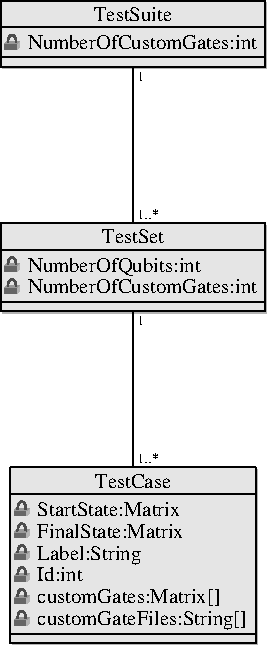
\includegraphics[height=0.4\textheight]{testsuitefig.pdf}
\end{minipage}
% \begin{emp}[classdiag](20, 20)
%   Class.A("TestCase")("-StartState:Matrix","-FinalState:Matrix","-Label:String","-Id:int","-customGates:Matrix[]","-customGateFiles:String[]")();
%   Class.B("TestSet")("-NumberOfQubits:int","-NumberOfCustomGates:int")();
%   Class.C("TestSuite")("-NumberOfCustomGates:int")();
%   % Class.D("SuperPositionalTestSet")()();
%   topToBottom(75)(C, B, A);
%   % D.n = B.s - (0, 50);
%   drawObjects(C, B, A);
%   clink(association)(C, B);
%   item(iAssoc)("1")(obj.nw = C.e);
%   item(iAssoc)("1..*")(obj.ne = B.w);
%   clink(association)(B, A);
%   item(iAssoc)("1")(obj.nw = B.e);
%   item(iAssoc)("1..*")(obj.ne = A.w);
%   % link(inheritance)(D.n -- B.s)
% \end{emp}
}
\caption{Test Suite Structures}
\end{figure}

Separate files are used to encapsulate the test suite specifications rather than including these in the Search Problem Manager configuration file, discussed in Section \ref{sec:manclasses}.
This separation follows the software engineering principle of modularity to ensure that the files remain readable and maintainable.
The framework is intended to improve the ability of researchers to reuse development or other researchers, the creation of test suite specifications can be seen as development.
With this modularity the distribution and reuse of test suite specifications will be much simpler than if the test suite specifications were embedded in the Search Problem Manager configuration file, discussed in Section \ref{sec:manclasses}.

% \begin{figure}
% \centering
% % \begin{emp}[classdiag](20, 20)
% % Class.A("TestCase")("-StartState:Matrix","-FinalState:Matrix","-Label:String","-Id:int","-customGates:Matrix[]","-customGateFiles:String[]")();
% % Class.B("TestSet")("-NumberOfQubits:int","-NumberOfCustomGates:int")();
% % Class.C("TestSuite")("-NumberOfCustomGates:int")();
% % % Class.D("SuperPositionalTestSet")()();
% % leftToRight(75)(C, B, A);
% % % D.n = B.s - (0, 50);
% % drawObjects(C, B, A);
% % clink(association)(C, B);
% % item(iAssoc)("1")(obj.nw = C.e);
% % item(iAssoc)("1..*")(obj.ne = B.w);
% % clink(association)(B, A);
% % item(iAssoc)("1")(obj.nw = B.e);
% % item(iAssoc)("1..*")(obj.ne = A.w);
% % % link(inheritance)(D.n -- B.s)
% % \end{emp}
% 
% \begin{emp}[classdiag](20, 20)
%   Class.A("TestCase")("-StartState:Matrix","-FinalState:Matrix","-Label:String","-Id:int","-customGates:Matrix[]","-customGateFiles:String[]")();
%   Class.B("TestSet")("-NumberOfQubits:int","-NumberOfCustomGates:int")();
%   Class.C("TestSuite")("-NumberOfCustomGates:int")();
%   % Class.D("SuperPositionalTestSet")()();
%   topToBottom(75)(C, B, A);
%   % D.n = B.s - (0, 50);
%   drawObjects(C, B, A);
%   clink(association)(C, B);
%   item(iAssoc)("1")(obj.nw = C.s);
%   item(iAssoc)("1..*")(obj.sw = B.n);
%   clink(association)(B, A);
%   item(iAssoc)("1")(obj.nw = B.s);
%   item(iAssoc)("1..*")(obj.sw = A.n);
%   % link(inheritance)(D.n -- B.s)
% \end{emp}
% \caption{Test Suite Class Diagram}
% \label{fig:testsuiteclassdiag}
% \end{figure}

The implementation of the test suite structure can be seen in Figure \ref{fig:testsuiteclassdiag}.
The custom matrices are held both as an array of Strings and of Matrix objects.
This is for no other reason than trying to recreate a test suite definition XML file in the form shown in Figure \ref{code:paulixtestset} requires the file name of the XML file specifying the custom unitary matrices and creating matrices from file each time they are needed in evaluation is very slow.
If there were just an array of Matrix objects the file names would be lost or require an additional array.
The inclusion of a second array was initially discounted as it would introduce an unnecessary source of potential bugs concerning the two arrays being ``out of sync''.
This would mean the Matrix objects may not represent the matrix encoded in the respective file as the Matrix objects are able to be modified and altered by the program without the file being updated.
To remove the potential for the two arrays to be out of sync, the matrix array is externally inaccessible and is only created by the constructors and the matrices are only able to be retrieved by index.
When the custom matrices are retrieved, the matrices are copied to ensure the matrix held in the test case cannot be altered by a malfunctioning component.

Alongside the framework, an independent test suite graphical editor is provided.
A user can use this to produce the XML file and therefore do not need to explicitly create the XML file.
The design and implementation of the graphical editor can be found in Section \ref{sec:indtestsuiteeditor}.

The contents of a test suite are not fixed.
If a user finds an error or wishes to add test cases, either a third party application or the provided test suite graphical editor can be used to update the respective test suite elements.
These changes need to be reflected in the XML file to become persistent so to ensure that the updated XML file is well formed the framework provides a class to produce from a given test suite.
This class is used in the independent test suite graphical editor and is recommended for use by any third party application.

When editing a test suite, if a test set for $n$ qubits is added to the test suite and the test suite already contains a test set for $n$ qubits, the two test sets are merged.
The test cases of the test set being added have their ID and labels modified so that they continue the sequence of the existing test cases already in the test suite.
When the test sets have to be merged the test cases are cloned.
This is in case the test set is used in a different test suite.
If this were not done, when the ID and label were modified they would also be updated in the second test suite.
This would cause unpredictable behaviour.

\subsection{Manager Classes}
\label{sec:manclasses}
As can be seen in the architecture diagram of the framework, Appendix \ref{sec:archdesign}, there are several classes with names suffixed with ``Manager''.
These classes provide access to the extendible areas of the framework.
There is a Manager class for the Suitability Measures, the Search Engines and the Search Problems.
Each of these are a specific site of expansion.

Each Manager is configured using an XML file specifying all options for the specific Manager.
The Fitness Function Manager will be configured for all the available Suitability Measures, the Search Engine Manager for all the available Search Engines, and the Problem manager for all the available Search Problems.
The Search Problem Manager class is outlined in detail in Section \ref{sec:problemman}.

The three managers are configured at runtime not at compile time.
This allows researchers to add suitability measures, search engines and search problems without recompiling the framework.
This runtime configuration provides a better plug-and-play design, a key foundation of the framework, compared to compile time configuration.
% Such knowledge separation encourages the use of the standardised interfaces specified for each expansion site.

\lstset{language=XML}
\begin{figure}
\begin{lstlisting}
 <FitnessFunc>
	<FitnessFunctionTag>
	  <Name>FITNESS FUNCTION NAME</Name>
	  <Class>IMPLEMENTING FULLY QUALIFIED CLASS NAME</Class>
	  <Desc>FITNESS FUNCTION DESCRIPTION</Desc>
	</FitnessFunctionTag>
</FitnessFunc>
\end{lstlisting}
\caption{XML for Suitability Measures Manager Configuration}
\label{code:fitfuntmanconfig}
\end{figure}

Figure \ref{code:fitfuntmanconfig} shows an outline of the XML file used to specify the available Suitability Measures.
The XML files specifying the available Search Engines and the available Problems can be found in Appendix \ref{sec:semanspecxml} and \ref{sec:probmanspecxml}.

These XML files are used to register the available implementations with the respective Managers.
The Manager classes use these registrations to provide the choice of available instantiations of Search Engines and Suitability Measures.

\begin{figure}
\centering
\begin{emp}[classdiag](20, 20)
Class.E("XYTag")("-Name:String","-Description:String","-ClassName:String")();
Class.F("XYManager")()("+getAvailableXYs():Set<String>","+getXY(String key):XY","+getSearchEngineDesc(String key):String");
leftToRight(75)(E, F);
drawObjects(E, F);
clink(association)(E, F);
item(iAssoc)("1")(obj.nw = E.e);
item(iAssoc)("1..*")(obj.ne = F.w);
clink(association)(F, E);
\end{emp}
\caption{Manager - Tag Class Diagram}
\label{fig:mantagclassdiag}
\end{figure}

Both the Search Engine and Search Problem Manager classes are implemented in the same way.
The class diagram in Figure \ref{fig:mantagclassdiag} shows the Manager design.
A mapping between the Name of the registered options and Tag objects is held in each Manager.
A Tag contains the information within the \lstinline{<XYTag> </XYTag>} element of the XML file.
\lstset{language=Java}
The \lstinline{getAvailableXYs()} method returns a set of strings, the registered names, rather than the XY Tags to ensure the Manager classes have full control over the creation of the managed elements.
To provide an XY object when requested using \lstinline{thegetXY(key)} method, the Manager classes use reflection to instantiate an object of the respective class, the value of the ClassName variable of the Tag registered with $Name=key$.

\subsection{Multiple Search Engines}
\label{sec:mulsearchen}
It is hoped the framework will be widely adopted by quantum algorithm researchers.
The framework is also aimed at researchers focussed on search techniques.
To perform comparisons between search techniques the framework needs to be able to use different search engine implementations.

Providing a simple interface that allows each researcher to potentially use a different search technique is likely to increase the tools applicability.
The simple interface allows a user to:
\begin{itemize}
 \item retrieve the names, used as the search engine identifier, of all registered Search Engines
 \item retrieve the instantiation of the specified Search Engine instantiation
 \item retrieve the description of the specified Search Engine
\end{itemize}

All registered Search Engines must implement the supplied interface.
The Search Engines are not restricted to evolutionary approaches.
The internal workings of the different search engines are unrestricted.

The alternative approach would have been to implement a series of search engines based on several different techniques and provide researchers this choice.
This was not accepted as it moved the tool away from the plug-and-play framework intended.

\subsection{Multiple Fitness Functions}
\label{sec:mulsuitmeas}
As was noted by Massey\cite{masseythesis}, different Fitness Functions can have a dramatic impact on the success of a Quantum Algorithm search.
The inclusion of a choice of Fitness Functions is to account for this.
As with Search Engines, the choice of Fitness Functions is provided by the Manager class through a simple interface with methods synonymous to those provided for the Search Engine selection.
A Fitness Function interface is provided to ensure that all Fitness Functions are able to be used universally within the tool and are not specific to any particular Search Engine for example.

Similarly to the Search Engine, a series of Fitness Functions could have been implemented and provided without provision for extension.
The justification for the approach taken is the same as listed for the multiple Search Engines.
It was deemed detrimental and in contradiction of the frameworks purpose to limit the Fitness Functions to those provided by the tool.


\subsection{Multiple Problems and Problem Specification}
\label{sec:problemman}
% As has been mentioned on several occasions, one of the foundation principles of the framework is the ability to ``Plug and Play'' the work of other researchers without the problem of integration.
% With Search Engines and Fitness Functions developed to adhere to the respective interfaces, a user should be able to work with the tool kit and treat it as a ``Black Box''.

Section \ref{sec:testsuitestruc} describes how test suites and all their contained test cases are specified in XML.
The use of XML files does however increase the effort required from the user.
The user needs to specify, each time they use the framework, the location of the XML file containing the correct test suite.
To reduce this effort the problem container is introduced alongside its manager.

The problem manager allows multiple problems to be defined within a single XML file so the user need not provide the test suite XML each time the framework is used.
This single XML file contains the definition of multiple problems.
An example of these XML files can be seen in Figure \ref{code:probmanconfig}.
A problem has a name, description and file name for the respective test suite XML file.
The name and description are used to provide a human readable explanation of the problem represented by the test suite XML file.
The use of a separate XML file to collate all defined problems makes maintenance much simpler.

Providing a problem manager allows the framework to be used for different problems without having to restart the system and without any external software needing to provide different problems explicitly.

\lstset{language=XML}
\begin{figure}
\begin{lstlisting}
<Problems>
  <prob>
    <Name>Final Pauli X</Name>
    <DefFile>config/finalpaulix.xml</DefFile>
    <Desc>A Pauli X gate on the final Qubit</Desc>
  </prob>
</Problems>
\end{lstlisting}
\caption{XML for Problem Manager Configuration}
\label{code:probmanconfig}
\end{figure}

The Search Problem Manager works in a similar way to the Search Engine and Suitability Measure Managers detailed in Section \ref{sec:manclasses}.
However, the difference between the registered Search Problems is the test suite configuration XML file rather than the implementing class.
A second difference is that the registered options are not static, a third party application can interact with the Manager to create new Search Problems and update the already registered Search Problems.
Therefore, the Search Problem Manager has to be able to produce an updated Search Problem Manager configuration file so the changes made are persistent.
The changes that the Search Problem Manager is concerned with is only updates to the values in the Search Problem Manager configuration file.
Any changes made to the set of Test Cases are not maintained by the Search Problem Manager.
This ensures that the different concerns are separated.
The update of Test Cases is detailed in Section \ref{sec:testsuitestruc}.

\subsection{Quantum Algorithms}
\label{sec:quantalgs}
The result of the searches are quantum algorithms.
To maintain the ``Plug and Play'' nature of the framework, the representation of these algorithms needed to be specified and standardised.
However, the representation also had to ensure that it was not limiting the search engines.

To provide a standardised and non-limiting representation the framework provides an internal quantum algorithm structure that can be simply built by any search engine.
This allows the search engines to have a different internal representation that is then used to build the standardised algorithm.
Using this there are no limitations on the structures used internal to the search engines.

The use of the standardised quantum algorithm also ensures that the reporting of an algorithm to the user is consistent.

\begin{figure}
\centering
 \begin{tabular}{|c|c|c|c|c|}
  \hline
Instruction & Gate1 & Gate2 & Phase & Sub-Algorithms \\
QuantumInstruction(Enumeration)&expnode&expnode&expnode&QuantumAlgorithm[]\\
\hline
 \end{tabular}
\caption{Quantum Instruction Structure}
\label{tab:quantinststruct}
\end{figure}

\begin{table}
\centering
 \begin{tabular}{|c|c|}
\hline
$exp \rightarrow e + e$ & $e \rightarrow exp$ \\
$exp \rightarrow e - e$ &  $e \rightarrow SystemSize$ \\
$exp \rightarrow e * e$ &  $e \rightarrow Value$ \\
$exp \rightarrow \frac{e}{e}$ &   \\
$exp \rightarrow e^e$ &   \\
$exp \rightarrow \frac{\pi}{2^{e\%10}}$ &   \\
$exp \rightarrow LoopVars[e]$ &   \\
\hline
 \end{tabular}
\caption{Expnode Context Free Grammar}
\label{tab:expnodecontext}
\end{table}

An algorithm is a list of instructions.
The instructions that are used in the standardised quantum algorithms take the form shown in Figure \ref{tab:quantinststruct}.
The list of values that the Instruction element can take can be found in Appendix \ref{sec:alginstructionlist}.
When the algorithm is reported to the user, it is reported as a list of instructions in the same form as is shown in Figure \ref{tab:quantinststruct}.
To improve readability, if a gate does not have a second gate, or use a phase or sub algorithms they are not reported to the user.
The textual form is also improved with the use of \{ and \} characters to denote the body of iterate instructions.
The $\frac{\pi}{2^{e\%10}}$ rule has the exponent modulo $10$ to improve the performance and also is to produce algorithms that are feasible.
Higher accuracy would require high presision hardware.
This value could be altered in the future to reflect the available hardware precision at any given time in the future.

$Gate1$, $Gate2$ and $Phase$ are all listed as being of type \emph{expnode}.
The type after evaluation for $Gate1$ and $Gate2$ is integer and for $Phase$ is double.
The \emph{expnode} type is required for these values to depend on value variables such as the system size and also loop variables.
The grammar that defines the \emph{expnode} type can be seen in Table \ref{tab:expnodecontext}.
The \emph{expnode} type is needed so that the algorithms can react to the parametrisation that provides the increased power when compared to quantum circuits.
As the circuit size is a variable a constant cannot be used for $Gate1$, $Gate2$ or $Phase$ as the value may depend on the circuit size and have to be calculated when a circuit is being built using the algorithm.

\begin{algorithm}
\begin{algorithmic}
\FOR{$i$ : $0\rightarrow{n}$ : $i++$} 
\STATE \COMMENT{You can use i here}
\FOR{$j$ : $0\rightarrow{m}$ : $j++$} 
\STATE \COMMENT{You can use i and j here}
\ENDFOR
\ENDFOR
\end{algorithmic}
\caption{Nested Loop Variable Access}
\label{alg:nestloopvars}
\end{algorithm}

% \lstset{numbers=left,language=Java}
% \begin{center}
% \begin{tabular}{c}
% \begin{lstlisting}
% for(int i = 0; i < n ; i++){
%   // You can use i here
%   for(int j = 0; j < n ; j++){
%     // You can use i and j here
%   }
% }
% \end{lstlisting}
% \end{tabular}
% \end{center}

With the inclusion of an loop control construct in the form of the \emph{iterate} and \emph{reviterate} instructions additional parameters are introduced.
In Java and many programming languages, as can be seen in the example of Java code above, when using nested loops access to all loop variables is provided, as shown in Algorithm \ref{alg:nestloopvars}.
This means that at line 2 the loop variable $i$ is able to be used but at line 4 both loop variable $i$ and $j$ can be used.
This nesting is quite a powerful language feature.
With the inclusion of the iterate instructions and therefore the possibility of nested iterations this loop variable access could be implemented in one of two ways.
The most na\"{\i}ve implementation would be to just allow access to the ``closest'' loop variable.
This would mean that the code at line 2 wouldn't be effected but the code at line 4 would no longer be able to use the $i$ variable.
The more sophisticated option, that is implemented, is to provide access to all loop variables.
This is a second parameter that requires the use of the \emph{expnode} type.
All current iteration variables are provided in a \emph{LoopVars} array.
As can be seen in Table \ref{tab:expnodecontext} the array is indexed by the value of a sub-expression.
To ensure that all indices requested are valid the value of the sub-expression is calculated using modulus \emph{LoopVars.length()}.
If the \emph{LoopVars} array has a of length $0$ the result is $0$ irrespective of the index requested.

The difference between the \emph{iterate} and \emph{reviterate} instructions is that \emph{iterate} counts from $1$ to $Gate1$ and \emph{reviterate} counts from $Gate1$ to $1$.
As is explained in Section \ref{sec:qubitnum}, the qubits are numbered from $1$ to $n$ which is why the iteration instructions count to and from $1$ rather than $0$ as is normal in Computer Science.
The two different iterate instructions are needed as they can express some looping constructs in a much simpler form that would be possible with just one of them.

For all \emph{Create\_*} instructions, $Gate1$ is used to index the qubit the actual gate should be assigned to.
Gate2 is only used by \emph{Create\_C*} and \emph{Create\_SWAP} instructions to index the control qubit and second qubit respectively.
For the \emph{Iteration} instruction, Gate1 is used for the number of iterations, $n$.
For the \emph{Create\_R*}, \emph{Create\_CR*}, \emph{Create\_P} and  \emph{Create\_CP} instructions, the Phase element is used to parameterise those gate to specify the amount of rotation applied by the resulting gate.

\subsection{Qubit Numbering}
\label{sec:qubitnum}
One of the major decisions made was way in which the qubits should be numbered.
The two options in respect to significance.

The chosen approach was that the identifiers increase with significance.
This means that for state $\ket{zy{\dots}ba}$ the qubit represented by $a$ would always have the identifier $1$ and the qubit represented by $z$ will always have the identifier equal to the system size.
For example, if the system size is three the identifier of the qubit represented by $z$ would be $3$.
This was chosen to ensure that an identifier always represents the same qubit, irrespective of the number of qubits in the system.

The discarded option was for the identifiers to increase as significance decreases.
This would mean that the qubit represented by $z$ would always be $1$ whereas the qubit represented by $a$ will always have the identifier equal to the system size.
Therefore with different system sizes the same identifier actually correspond to qubits of different  significance.

The justification for this choice is to make the algorithm simpler.
If the identifiers were dependant on the number of qubits it would make the understanding algorithm slightly more involved.

The use of this numbering is also much more natural as the identifier, $x$, of a qubit, $a$, is related to the value of the qubit when read in binary.
The value of the qubit $a$ is $2^{x-1}$.
This makes the optimisation of gate application, see Section \ref{sec:quantumgates}, much simpler.

The identifiers start at $1$ rather than $0$.
This allows the value $0$ to be used as the flag within the framework to indicate that the system size should be used.
For example the instruction \emph{Create\_H 0} would create a Haramard gate on the qubit with the identifier equal to the system size, highest significant qubit.
The use of $0$ allows the integer type to be used without additional flag types to complicate the framework and algorithms.

\subsection{Quantum Circuits}
\label{sec:quantumcircuits}
To perform the evaluation of an algorithm the circuits for the test sets need to be produced.
Both the representation of the circuit and the mechanism to construct the circuit from the algorithm needed to be standardised to ensure the ``Plug and Play'' nature of the framework.

The framework provides a default circuit builder and allows a separate circuit builder to be provided as long as it conforms to the interface and the circuits it produces also adheres to the respective interface.
There is no manager class provided for circuit builders.
This was due to an assessment of the intended uses of the framework.
It is intended that the framework would be used primarily to perform the following:
\begin{itemize}
  \item Perform research into the effect of different fitness functions on the search for quantum algorithms
  \item Perform research into different search techniques that could be used to produce quantum algorithms
  \item Perform research to produce new quantum algorithms for a specific problem
\end{itemize}

It is not seen as a priority of the system to provide the same level of flexibility to the circuit building as the search engines and fitness functions.

The provided circuit builder has several rules.
Firstly, for $Gate1$ and $Gate2$ the absolute value of the \emph{expnode} expression is used as there are no qubits with negative indices.
Secondly,For $Gate1$ and $Gate2$ the \emph{expnode} expressions, see Section \ref{sec:quantalgs}, can evaluate to $0$, however due to the way the qubits are numbered, see Section \ref{sec:qubitnum}, there is not a qubit with identifier $0$.
As is mentioned in Section \ref{sec:qubitnum} the number $0$ is used as the \emph{System\_Size} flag so if $Gate1$ or $Gate2$ were to evaluate to $0$ it would be replaced by the value of \emph{System\_Size}.
Thirdly, in contrary with the decision taken by Massey\cite{masseythesis}, if the \emph{expnode} expression evaluates to more than \emph{System\_Size} that value won't be coerced to \emph{System\_Size} but the instruction shall just be skipped.
The result of these three tackles the problem outlined by Clark and Stepney\cite{Stepney07searchingfor} of unequal identifier representation.
With these three simple rules each qubit identifier and the \emph{System\_Size} flag are represented by two elements.
Each qubit identifier is only represented by the identifier and the negative value of the identifier.
The \emph{System\_Size} flag is represented by the dedicated \emph{System\_Size} value and if an \emph{expnode} expression evaluates to $0$.

A simple circuit optimiser is built into the provided circuit builder.
Using static knowledge about which of the gates shown in Table \ref{tab:providedgates} are self reversing the circuit builder builds higher efficiency circuits.
This is performed by removing elements such as
$
\Qcircuit @C=1.0em @R=.7em {&\gate{H}&\gate{H}&\qw}
$
that do not have any affect on the state.
However it cannot perform these improvements if there are any gates, even on different qubits, between the gate pairs that could be remove.

The circuits that are produced by a circuit builder are hidden behind an interface.
This is to allow third party circuit builders to use their own internal representation and also to allow any future optimisations made in future work on this framework to be made without impacting the work of researchers.

The circuits produced provide the represented quantum circuit as an ordered iterator of quantum gates.
The use of an ordered iterator rather than a specific data structure is to ensure that any future optimisation or third party circuit representation is not limited.
It also reduced the potential errors involving the interpretation of a more complex data structure.

The circuits also provide a Latex representation to allow the circuit to be visualised.
The Latex representation uses the QCircuit package that can be freely obtained at \cite{QCsite}.

The circuit implementation, \emph{basiccircuit}, provided in the framework is implemented as a simple ordered list.
It uses the Java provided \emph{LinkedList} implementation.
The use of a list implementation ensures that the number of gates is almost unlimited until the heap is exhausted.
With this implementation there is no difference in the representation between a circuit for a system size of 1 or a system size of 1000.
The only affect  the system size has is during unitary application to a quantum state, see Section \ref{sec:quantumgates}.

\subsection{Quantum Gates}
\label{sec:quantumgates}
Any quantum circuit will be a series of quantum gates on specified qubits.
The quantum gates provided by the system are hidden behind an interface.
This is to ensure that any future optimisation of any gate's implementation cannot interfere with the implementation of any other component of the system.

Each quantum gate is required to provide a unitary matrix but it is not required that the matrix must be used in the application of the gate.
For quantum circuits with a high number of qubits, the cost of simulation increases rapidly.
This is mainly due to the increase in state vector and unitary matrix sizes.
Matrix multiplication is used to apply a unitary operation to a state vector, yet it is a very expensive operation.

To improve the performance optimisations can be applied for several gate types.
This is most obvious when analysing the operation of the Pauli X gate.
Figure \ref{eq:paulixcheaptrickvisual} shows, with the help of colour, that the application of a Pauli X gate on Qubit 1 is essentially a flip of neighbouring values.
This is also true for a Pauli X gate on any other qubit, just the definition of a state's ``neighbour'' is modified with respect to the identifier of the qubit on which the gate is applied.

% l' unite
\newcommand{\myunit}{0.5 cm}
\tikzset{
%     node style sp/.style={draw,circle,minimum size=\myunit},
    node style ge/.style={circle,minimum size=\myunit},
%     arrow style mul/.style={draw,sloped,midway,fill=white},
%     arrow style plus/.style={midway,sloped,fill=white},
}

\begin{figure}
\centering

% \tikzstyle{every picture}+=[remember picture]
% \tikzstyle{na} = [shape=rectangle,inner sep=0pt]
% \tikz\node[na](word1){John}; loves \tikz\node[na](word2){his}; mother.
% \begin{tikzpicture}[overlay]
%   \path[->,red,thick](word2) edge [out=90, in=90] (word1);
% \end{tikzpicture}
% \[
% \begin{tabular}{ r c l }
%   \(\begin {pmatrix}
%    \textcolor{blue}{ \tikz\node[na](word3){a} } \\
%     \textcolor{red}{b}
%   \end{pmatrix}\) 
% & 
%   \(\rightarrow\) 
% & 
%   \(\begin {pmatrix}
%     \textcolor{red}{b}\\
%     \textcolor{blue}{ \tikz\node[na](word4){a} }
%   \end{pmatrix}\) \\
% 
% \\
% 
%   \(\begin {pmatrix}
%     \textcolor{blue}{a}\\
%     \textcolor{red}{b}\\
%     \textcolor{green}{c}\\
%     \textcolor{cyan}{d}
%   \end{pmatrix}\)
%   & \(\rightarrow\)
%   & \(\begin {pmatrix}
%     \textcolor{red}{b}\\
%     \textcolor{blue}{a}\\
%     \textcolor{cyan}{d}\\
%     \textcolor{green}{c}
%   \end{pmatrix}\) \\
% \end{tabular}
% \]
% \begin{tikzpicture}[overlay]
%   \path[->,red,thick](word3) edge [out=90, in=90] (word4);
% \end{tikzpicture}


% \subfigure[1 Qubit]{
\begin{tikzpicture}[>=latex]
% les matrices

\matrix (A) [matrix of math nodes,
             nodes = {node style ge},
             left delimiter  = (,
             right delimiter = )] at (0,0)
{
  a \\
  b \\
};
\node [below=10pt] at (3*\myunit,-3*\myunit) 
    {1 Qubit};

\matrix (B) [matrix of math nodes,%
             nodes = {node style ge},%
             left delimiter  = (,%
             right delimiter =)] at (6*\myunit,0)
{%
  b  \\
  a \\
};
% \node [draw,above=10pt] at (B.north) 
%     { $B$ : $p$ rows \textcolor{red}{$q$ columns}};

% les fleches
% \draw[<->,red](A-2-1) to[B-1-1]
% 	node[arrow style mul] (x) {$a_{21}\times b_{12}$} (B-1-2);

\draw[->,red](A-2-1) to (B-1-1);
\draw[->,red](A-1-1) to (B-2-1);


\matrix (C) [matrix of math nodes,
             nodes = {node style ge},
             left delimiter  = (,
             right delimiter = )] at (12*\myunit,0)
{
  a \\
  b \\
  c \\
  d \\
};
\node [below=10pt] at (15*\myunit,-2*\myunit) 
    {Pauli-X on Qubit 1};

\matrix (D) [matrix of math nodes,%
             nodes = {node style ge},%
             left delimiter  = (,%
             right delimiter =)] at (18*\myunit,0)
{%
  b  \\
  a \\
  c \\
  d \\
};

\draw[->,red](C-2-1) to (D-1-1);
\draw[->,red](C-1-1) to (D-2-1);
\draw[->,blue](C-4-1) to (D-3-1);
\draw[->,blue](C-3-1) to (D-4-1);

\matrix (E) [matrix of math nodes,
             nodes = {node style ge},
             left delimiter  = (,
             right delimiter = )] at (24*\myunit,0)
{
  a \\
  b \\
  c \\
  d \\
};
\node [below=10pt] at (27*\myunit,-2*\myunit) 
    {Pauli-X on Qubit 2};

\matrix (F) [matrix of math nodes,%
             nodes = {node style ge},%
             left delimiter  = (,%
             right delimiter =)] at (30*\myunit,0)
{%
  c  \\
  d \\
  a \\
  b \\
};

\draw[->,red](E-1-1) to (F-3-1);
\draw[->,blue](E-2-1) to (F-4-1);
\draw[->,red](E-3-1) to (F-1-1);
\draw[->,blue](E-4-1) to (F-2-1);

\node [below=10pt] at (21*\myunit,-3*\myunit) 
    {2 Qubits};
\end{tikzpicture}
% }

\label{eq:paulixcheaptrickvisual}
\caption{Visual Representation of Direct Vector Manipulation Equivalent of Pauli X Operation}
\end{figure}

The use of these tricks is not specified but the interface has been designed to ensure that the gate implementations can use such tricks or matrix multiplication interchangeably.
The interface includes an \emph{apply} method that takes an initial state and returns the state after the application of the gate.
This ensures that only the gate implementation needs to understand how the circuit should be applied.

Each gate must also provide a QCircuit \cite{QCsite} representation to produce the QCircuit representation of the entire circuit.

The implementations for gates that affect two qubits are hidden by an extended interface to provide access to the identifier of the second qubit but ensures that all standard gate operations are also available.

\begin{table}
\centering
% \[
\begin{tabular}{ | c | c || c | }
\hline
\multicolumn{2}{|c||}{\textbf{Matrix Manipulation}} & \textbf{Direct Vector Manipulation} \\ \hline
Phase Gate & W Gate &Hadamard \\ \hline
RX Gate &Custom U Gate & Pauli X \\ \hline
RY Gate &Controlled U Gate & Pauli Y \\ \hline
RZ Gate &Swap & Pauli Z \\ \hline
V Gate && \\ \hline
\end{tabular}
% \]
\caption{Gate Implementation}
\label{tab:gateimps}
\end{table}

As has been mentioned, a number of the gates shown in Table \ref{tab:providedgates} can be implemented either as a matrix multiplication or a direct vector manipulation.
Several of the gate implementations in the framework use the direct vector manipulation and others use the matrix multiplication.
The table in Table \ref{tab:gateimps} shows which of the provided gates are implemented using the matrix manipulation and which use the direct vector manipulation.
Some of the algorithms used by to perform the direct vector manipulation were based on those used in jQuantum\cite{jquantum}.
For all gates that use matrix multiplication their equivalent unitary is based on those listed in Table \ref{tab:providedgates} but has to adapt to the qubit they are applied to and the system size.
The equivalent matrix is calculated in two sections.
The initial section is the construction of the matrix listed in Table \ref{tab:providedgates}.
This initial section is calculated in the constructor of each gate.
The gate on which the gate is applied is provided as an argument to the constructor of the gate.
Unfortunately a Java interface cannot specify the signature of the constructor of implementing classes and abstract classes require the constructor to be fully defined which is not possible when the constructor needs to perform this first section.
As a result this cannot be ensured but is expected as part of implementing the interface.
The second section is the combination of the matrix constructed in the initial phase and identity matrices for all qubits not effected by the gate.
This second section is performed as part of the \emph{apply} method.
The second section carried out in the \emph{apply} method does not impose any restriction on the system size.

% There are several gate implementations that deserve a more detailed summary.
To produce the unitary matrices shown in Table \ref{tab:providedgates} for the RX, RY and RZ gates the matrices of other gates are used.
Equations \ref{eq:rxcalc} - \ref{eq:rzcalc} shows the details of these matrix calculations.
These equations are taken directly from Lecture 9 of \cite{QIPLect}.
\begin{eqnarray}
\label{eq:rxcalc}
 R_x(\theta)&=&\cos{\frac{\theta}{2}}I-i\sin{\frac{\theta}{2}}X \\
\label{eq:rycalc}
 R_y(\theta)&=&\cos{\frac{\theta}{2}}I-i\sin{\frac{\theta}{2}}Y \\
\label{eq:rzcalc}
 R_z(\theta)&=&\cos{\frac{\theta}{2}}I-i\sin{\frac{\theta}{2}}Z 
\end{eqnarray}

The second gate implementation that requires a more detailed summary is the Controlled U Gate.
The implementation of the gates cannot assume that the circuit that is produced by an algorithm is correct.
Placing all the restrictions on the search process that need to be placed on the circuit would have a serious impact on certain search processes.
Therefore all the restrictions need to be handled by elements of the framework.
If the U gate affects more that a single qubit, possible with custom matrices, it would be possible for the U operation to affect the qubit specified as the control qubit.
It was decided that a restriction for Controlled U Gates would be added.
The restriction added was that the control qubit cannot be affected by the U operation.
If the specified qubit would be affected by the U operation the implementation acts as though it was an uncontrolled U gate.
A second consideration for the design and implementation is if U is a custom gate the U matrix can change.
This means that the calculation of the matrix that represents the controlled version of U needs to be able to update depending on the test case.

A major implementation detail is how the matrix that represents a controlled version of unitary U is calculated.
The calculation changes depending on the relative position of control qubit.
If the control qubit is a higher significant qubit the calculation is different than if the control bit is a lower significant qubit.
Equation \ref{eq:clu} is the calculation if the control qubit is a lower significant qubit.
Equation \ref{eq:chu} is the calculation if the control qubit is a higher significant qubit.
$S1$ is an identity matrix of the size $2^n$ where $n$ is the number of lower significant qubits that aren't the target or control bits or between the control qubits and effected gates.
$S2$ is an identity matrix of the size $2^n$ where $n$ is the number of higher significant qubits that aren't affected by the Controlled U gate, a control bit or between the control qubits and effected gates.
U is the matrix that defines the operation of the gate under control.
This unitary matrix is retrieved using the \emph{getUnitary} operation on an object of the correct class.
The \emph{getUnitary} operation returns the matrix created by the first section explained previously in this section.

\begin{eqnarray}
\label{eq:clu}
 CU&=& ((\begin{pmatrix}1&0\\0&0\end{pmatrix}\otimes S1)+(\begin{pmatrix}0&0\\0&1\end{pmatrix}\otimes U) \otimes S2) \\
\label{eq:chu}
 CU&=& (( S1 \otimes \begin{pmatrix}1&0\\0&0\end{pmatrix})+(U \otimes \begin{pmatrix}0&0\\0&1\end{pmatrix}) \otimes S2)
\end{eqnarray}

Equations \ref{eq:clu} and \ref{eq:chu} are generalisations of the Controlled-U gate that have not previously been published.

With the calculation being flexible for any gate U there is an additional  scenario that must be considered.
When the control qubit would be affected by the application of the gate, due to the gates size being greater that $1$ or the control and target qubit identifiers being equal, the control is removed.
This results in a standard U gate without any controlling qubits.

As with standard gates, the calculation of the full matrix is performed in two stages as previously described in this section.
If U is a Custom gate then the full matrix is performed in a single stage as described in Section \ref{sec:custgates}.

\subsection{Custom Gates}
\label{sec:custgates}

As has been explained in Section \ref{sec:testsuitestruc}, the framework has to provide a way to include custom gates.
The way of specifying the custom unitary matrices is explained fully in Section \ref{sec:testsuitestruc}.
Each custom gate has an identifier between $0$ and $n-1$ where $n$ is the number of custom gates defined for the respective test suite, see Section \ref{sec:testsuitestruc}.

To use these custom unitary matrices, the framework provides a gate implementation called \emph{Custom\_Gate}.
This is significantly different from all other gates in one particular feature.
All gates listed in Table \ref{tab:providedgates} have a fixed unitary matrix and only have to adapt for the number of higher significant qubits that are not effected by the gate.
This is not so for custom gates, their operation change on a test case by test case basis and therefore both the ``phases'' mentioned in Section \ref{sec:quantumgates} are performed during the \emph{apply} method.

The \emph{apply} method in the Gate interface has two parameters, one is the quantum state on which the custom operation is applied and one that is the test case.
The test case is provided to extract the custom matrix for the custom gate's identifier.
If the custom gate identifier is invalid, $<0$ or $n\geq$, an array out of bounds exception is thrown.
If this exception is caught, both the \emph{apply} and \emph{getUnitary} methods behave as though the matrix returned were the identity matrix.

Using the test case that is supplied as an argument, the \emph{apply} method uses an argument provided to the constructor of the gate as in parameter to the \emph{getCustomGate} method of the test case.
The full unitary matrix, including identity padding for unaffected qubits, is produced using the matrix retrieved from the test case.
The state is multiplied by this unitary matrix to produce the return state.

The \emph{getUnitary} method also uses the test case provided to retrieve the matrix from the test case using the custom gate identifier.

The unitary matrices that each test case provides are not guaranteed to affect the same number of qubits.
As a result the production of the QCircuit representation cannot be guaranteed to represent the exact affect of a custom gate.
The framework therefore treats all custom gates as equal.
The lowest number of qubits they can affect is $1$.
As a result the framework shows all custom gates as single qubit gates on the lowest significant qubit that they affect.

\subsection{Search Engine Parameters}
With many search techniques there are a number of parameters that can be configured and altered, sometimes having dramatic effects on the search results.
To enable the configuration of these parameters through the framework a suitable, and flexible method had to be introduced into the design.
Not all search techniques have the same number of parameters to configure and due to search engines being developed potentially by different researchers, even if the parameters are the same, their internal representation may be different.

The framework requires a search engine to provide two \emph{search} methods that start the search process.
The first takes two arguments and is intended for use within third party applications that want full control over GUI components or do not provide a GUI.
The first argument is a boolean array.
This is an array with a length equal to the number of gates in the \emph{QuantumInstructionEnum} enumeration.
The value at each index indicates whether the element of the \emph{QuantumInstructionEnum} enumeration with the same index should be included in the search and therefore allowed in the result.
The second is an Object array.
This second array is provided to allow search engine researchers to have search engine parameters that are configured by a third party application.
The array more cannot be more specific that an Object array.
If the array were more specific, a String array for example, all parameters would have to be expressible in the chosen representation.
This could restrict the parameters available for the researchers to provide.
An Object array is so general that any parameters can be expressible.
However, it places responsibility on the researcher to provide adequate documentation and explicit error messages with regards to the ordering and the type of the parameters required by the individual search engine.

The second \emph{search} method takes no arguments.
It is intended to either launch a search parameter dialog to modify the search parameters.
The dialog should start the search process after all parameters have been specified.

% If a search engine comes under the second category and is providing a graphical user interface, the system must be run on a system configured to allow GUIs to be displayed.
This second method ensures the parameter dialog is entirely in under the control of the search engine implementer.
% The configuration of the user interface is controlled entirely by the search engine rather, than any third party software or the framework.
It is assumed that the person with best understanding of the parameters provided by a search engine is the implementer.
This aims to improve the user interface with respect to the structure principle, see Section \ref{sec:provgui}, as the search engine implementer can structure the dialog to group similar parameters.
The ordering of parameters in the Object array of the first \emph{search} method cannot be assumed to be a good indication of grouping and there is no explicit separation of groups.
As a result if the framework, or a third party client, were to provide an the automated dialog generator the similar parameters may not be grouped.

A second justification is the aim of a ``Plug and Play'' framework.
If the dialog was included as part of third party software, or even by the framework, it would have to be adapted for each search engine implementation or be generated automatically.
Automatic generation is unlikely to produce a ``principled'' user interface, see Section \ref{sec:provgui}.
The modification of the framework and third party clients for each search engine is not acceptable and is totally incompatible the principle of ``Plug and Play''.
% With such a design it is likely that the research community would see no advantage to using the framework than working as they are now, in complete isolation.

\subsection{Design as a Black Box}
\label{sec:thirdpartyblackbox}
The framework is designed to be used as a black box.
All external code is allowed access only through the interfaces and final or abstract class types.
The implementation of the internal framework functionality is hidden and not required by third party software.
This design ensures that third party software shall be loosely coupled with the framework.

Likewise, all internal modules (algorithms, circuit builders, circuits, gates, circuit evaluations, etc) are also designed to view each other as black box modules.
This improves the modularity and reduces the coupling between these internal modules.

\subsection{Algorithm and Circuit Evaluation}
\label{sec:cireval}
When an algorithm is produced by a search engine, the circuit is built for each test set.
This circuit then needs to be evaluated against all test cases held in the respective test set.
As mentioned in Section \ref{sec:testsuitestruc} the framework uses a start and final state pair to define the desired operation of the algorithm.
Therefore the framework must provide the simulation of an arbitrary circuit on and arbitrary start state.

Due to the design decisions taken previously all the functionality is provided and just needs a simple management process, this is provided by a class implementing the \emph{circuitevaluator} interface.
A basic implementation is provided and third party implementations can also be used.

With the circuit interface providing an ordered iterator over the gates in the circuit, and each gate providing an \emph{apply} method the circuit evaluator just needs to work through all the gates in the iterator and calling the \emph{apply} method with the returned state of the previous call.
To evaluate the circuit against a test case, the process simply needs to use the start state provided by the test case as the argument of the \emph{apply} method of the first gate.
The state returned by the final call to the \emph{apply} method is a state equivalent to the quantum state that would exist if the circuit were to be produced and provided with the same initial state.

The suitability measures have a very simple interface.
They only provide a method to retrieve the name of the suitability measure and a method to produce a numerical measure of similarity between two quantum states.

Using the selected suitability measure the final state produced by the circuit is compared to the expected final state defined in the test case.
Repeating this process for all available test cases in the current test suite, a numerical and therefore comparable suitability value can be assigned to any algorithm produced by the search engine.

This is one example where the design of the framework ensures that the when combining all the elements of the framework (the gate, the circuit, the test cases etc) the logic required is simple.
This improves the readability of the code and therefore is likely to improve the quality of the code.
With higher readability the number of software bugs are likely to be reduced due to higher levels of understanding.

It is assumed that when a researcher creates a test suite, the test cases that are included are those that the have a higher interest in.
As a results it can also be assumed that the researcher would be interested in the final state produced by the best solution found by the search engine for all the start states provided by the test suite.
The circuit evaluator interface provides a simple method call to produce these.
The \emph{getResults} method returns a test suite data structure that is almost identical to that provided by the search problem used in the search.
The only difference is that the final state of each test case in the returned structure is not the desired theoretical state but the actual final quantum state produced by the circuit simulation.

\subsection{Step-By-Step Evaluation}
\label{sec:sbsecireval}
The framework is required to provide a step-by-step evaluation facility.
There are two abstract ways this can be provided.
The framework can provide an interactive process that only applies a gate when it receives the command to do so and reporting the ``current state''.
The second option is to record the ``current state'' at each point in the circuit.

The main advantage of the first method is that it doesn't require processing of gate applications if the interactive evaluation does not reach them.
A second advantage is that the memory requirement is very small as only the ``current state'' and the position in the circuit the evaluation is up to.
A disadvantage is that for complex gates the application of the unitary operation could take longer than it is acceptable for a user to wait.
A second disadvantage is that if the memory required is kept to the minimum, moving backward will also require the application of a gate.
However, the gate that needs to be applied is not necessarily the same gate that is applied when working forward.
This could make the step-by-step evaluation quite complex to implement.
The time required for the reversed gate to be calculated and applied could also be an issue for responsiveness.

The main advantage of the second alternative is that to move forward, and also to move backward, is a simple loading of the respective ``current state'' from a data structure.
This results in the requests from the user to move forward and backward in the circuit taking approximately constant time irrespective of the stepped over gate's complexity.
A second advantage is that taking a step backward in the evaluation never requires the inverse of a gate to be calculated.
For gates such as the Pauli gates this is not an issue as they are their own inverse.
However this is not the case for arbitrary gates requiring the inverse of arbitrary matrices to be calculated.
The main disadvantage of the trace method is that the memory requirements are not constant, they are linear with respect to the number of gates in the circuit but exponentially with respect to the number of qubits in the system.
The second disadvantage is that although stepping through a circuit does not require the application of gates to the ``current state'', the full trace has to be produced before the step-by-step evaluation can be performed.
This means that if the circuit produced is large and complex, the start up and initialisation time could be significant.
The requirement for the full circuit to be evaluated irrespective of how many steps are taken in the step-by-step evaluation could lead to trace elements never being reached.

The way the framework has been designed is to include the second of these two options.
The additional memory requirements are not likely to be excessive when viewed in respect to the amount of RAM available in the average PC.
The main reason for the choice was that the calculation of all ``current state''s is done once and can be accessed as many times without extra computation required.
This should make the responsiveness if the framework much better.

There is also a second major design decision to be made with respect to the step-by-step evaluation, what the initial state should be to produce the trace.
There are really two alternatives.
The initial state could either be provided by the user explicitly or the test cases of the search problem could be used as the source of the initial  states.

The decision was made to combine the two options.
The framework accepts as an input to the step-by-step tracer a test suite data structure.
The test suite can either be the same that was provided by the Search Problem and used by the suitability measure or can be a new test suite that has been created.
This allows the client or third party application to provide either or both of the options.

The circuit evaluator interface provides the \emph{getTrace} method that provides a list of test sets.
The step-by-step evaluation is performed on a circuit rather than an algorithm.
This means that only test cases for a specific number of qubits can be stepped through together, this is why the list is of test sets rather than test suites.
It would have been possible to produce the traces for all test sets in the test suite and then returned a list of test suites.
This was not implemented as it is likely that a researcher would try and understand each circuit in turn and then look for how they related as a second phase.
The step-by-step evaluation is expected to aid in the understanding of the circuits rather than the comparisons.
Therefore if a researcher had produced a large test suite, and is only concerned with the understanding of a particular circuit, the wait for the trace to be produced for the full test suite is likely to be significantly longer than for just the relevant test set.

The implementation of the circuit evaluator that provides this trace runs through each test case in turn.
After each gate has been applied, the ``current state'' is set as the final state attribute of a cloned version of the current test case that is subsequently added to the returned data structure.
The implementation is purely concerned with providing the trace, not suitability measure evaluation is performed.

As mentioned in Section \ref{sec:cireval}, the design of the framework makes the creation of this trace much simpler.
The separation of concerns makes the tracing logic much simpler and much less obscured than it would have been if design decisions regarding the gate and circuit interfaces had not been made.

\subsection{Batch and Distributed Processing}
The framework produced is not expected to be used solely for Quantum Algorithm research.
It is also expected to be used for research into the search techniques themselves.
Therefore, the framework had to provide a managed solution to perform multiple jobs, a batch, and for the results to be collated for statistical analysis.

The search engine interface provides a \emph{getResults} method that returns an array of search results produced by the last call to a \emph{search} method.
The \emph{search} methods do not return the array themselves so the method is not a blocking call.
To ensure clients are informed when the results are available, the search engine requires any client to register as an observer.
This decision was taken so that clients did not have to provide the non-blocking mechanism.

The framework has been designed so as not to provide any additional help for batch processing for a very simple reason.
The way that batch processing is carried out is not constrained.
This allows the researcher to select how each iteration should be processed and what statistics need to be collected at which stage.
If the framework were to fully manage the batch operation researchers would be restricted.

For example, the framework could be implemented to sequentially execute each job.
For a researcher who has access to a cluster this could be highly frustrating.
Due to the complete separation of each job, there is no inter-job communication, it is perfectly suited to distribution.
It is effectively a Monte Carlo experiment.
However, if the framework were to provide a distributed computing mechanism, the researchers would be forced to use this.
This would mean that even if the chosen framework would be highly inefficient for a specific search technique or even if it was highly inefficient when running in a local mode there would not be any option available to the researcher other than to modify the framework.
This is obviously not desirable from a ``Plug and Play'' perspective.

This does however have the impact that different researchers could use different distribution frameworks.
If they are fully managed by the search engine this is not a problem but if they require additional configuration it does detract form the ``Plug and Play'' nature of the framework.
As a result a recommendation is made for all search engines produced for the framework to be implemented as a local version alongside any distributed implementation.
% This means that if a researcher wishes to use the search engine on a single machine or on an incorrectly configured cluster the application can still proceed.
% This is likely to have an impact on performance when compared to it the same search being performed on a correctly configured cluster.

The prescription of a batch processing manager may also restrict the ability to collect statistics.
Different researchers may require different statistics.
The reporting of statistics is not provided by the framework but search engines for this reason.

Both of these decisions may appear to reduce the power of the framework and the reasons to use it.
However, it is easy to argue that the management of batch distribution and statistical reporting would increase the power of the framework but seriously undermine the usability of the framework and therefore is unlikely to be adopted by researchers.

\section{Provided Tools}
The research framework is accompanied with two independent tools.
These are not intended to take the place of a third party client.

All of the configurations for manager classes and encodings of stored test suites and matrices are stored in XML.
The configuration files for the manager classes are relatively simple and are unlikely to be hard to produce manually.
However, the encoded test suites and matrices are likely to require longer XML files.
To improve the efficiency of the researcher and to reduce the probability of simple, but hard to spot, errors being introduced graphical editors are provided alongside the framework.

\subsection{Graphical Test Suite Editor}
\label{sec:indtestsuiteeditor}
A meaningful test set is likely to contain at least 4 test cases, but usually many more.
Say for example that the 4 test cases are all for the system size of 2.
This results in 4 test cases, each with 2 matrices each containing 4 complex numbers.
This would require an XML file to contain 64 floating point numbers, as complex numbers are stored in the XML file as two floating point values.
Remember that this is a test suite of just 4 test cases acting on 2 qubits, the number quickly increases with the system size and number of test cases.
Writing this XML file by hand in a text editor is not only tedious, but error prone.

To reduce the tedium of the process and the number of errors a graphical user interface is provided.
The interface is simple and clear, not providing the user with anything that is not necessary.
The interface allows the user to either edit a test suite that is already encoded in a file, or to create a new test suite from scratch for up to 10 qubits.
The limit is not imposed by the framework but by the editor.
Any test suite containing test cases of greater than ten qubits, the final state is likely to have been calculated by a third party application and manual input of $2^{11}$ complex numbers for both a starting and final state is likely to introduce errors.
Therefore it is recommended that time is spent integrating the third party software and the framework so the test suite can be automatically generated.

A user can add and remove test sets and test cases.
Each test set is provided on a separate tab.
The state is represented by a $2^n\times{1}$ matrix.
This makes the simple tabular visualisation used to edit the starting and final states the natural choice.
Two tables are used, one to edit the starting state and one to edit the final state.
The complex numbers are not listed as two separate floating point values but in Cartesian form.
When a user has created or made the changes, the test suite can be saved to an XML file.
The XML file is one that matches the format defined in Section \ref{sec:problemman} and also contains comments to try and improve the understanding if it were to be read using a simple text editor.

The design of the editor follows the user interface design principles, see Section \ref{sec:provgui}.
The editor is very simple with no extraneous functionality.
The use of tabs ensures that the editor design is structured, all related test cases are shown together and all user controls are also grouped whether they act on the test suite as a whole or the current test set and test case.
The two tables use the same class and each tab is also of the same class ensuring consistent visual representation and component reuse.

\subsection{Graphical Matrix Editor}
\label{sec:indmatrixeditor}
As with the number of floating point values required to define a test suite, the number required to define a matrix rapidly grows with the number of qubits.
This makes the manual production of the defining XML files again tedious and error prone.
The matrix encoding in file is optimised so that only non-zero values are stored in the file potentially reducing the number of values required.
This improves the process slightly but is can still be seen as rather tedious and error prone.

The framework provides a very simple editor that can be used to create the XML files in a much more familiar way.
The editor allows users to edit a matrix currently encoded in a file or to create a matrix of up to four qubits from scratch.
This is not a limit imposed by the framework.
It is to try and encourage the integration with third party applications.
For gates acting on four qubits the matrix contains $256$ complex numbers, for gates acting on five qubits this increases to $1024$.
Manually inputting $1024$ complex numbers into a table with $32$ columns and $32$ rows makes it very easy to make a mistake.
For operations of this size it is likely the matrix would have been calculated by a third party application.
This limit on the editor is to try and increase the integration with third party applications and therefore reduce errors.

\section{Search Engine Implementations}
\label{sec:provsearcheng}
\subsection{Q-Pace Based Search Engine}
Alongside the framework, a search engine based on the Q-Pace IV search engine featured in \cite{masseythesis} has been developed.
This is a Genetic Programming based search engine using the Java-based Evolutionary Computation Research System ECJ\cite{ecjtool}.

The search engine is provided in both local and distributed versions.
The local version uses separate threads to serially perform iterations.
The distributed version uses the JPPF Framework\cite{jppfweb} to perform iterations in parallel using all resources available.
To ensure that the function of both the local and distributed versions are the same, the two versions are based on the same code parametrised by the container class for the processing, Thread or JPPFJob.
The processing unit is implemented as a search engine core that implements the JPPFTask interface, which inherits the Runnable interface.
This allows the processing unit to be used both for the local and distributed version ensuring consistency.

The JPPF Framework was chosen for the distribution as it is very simple to configure and provides the functionality required in a very easy to understand way ensuring code readability is maintained.
There are many other frameworks available as well as producing a bespoke distribution system.
The bespoke solution was rejected as it is completely opposed to the philosophy behind the framework.
Other open source frameworks, including Apache Hadoop\cite{apahadoop}, were not chosen as they provided much more functionality than is required and as a result were more complex.
They also required significantly more additional statements within the functional source code to orchestrate the distribution and therefore more intrusive.

The statistics panel provided by the search engine reports the generation that the ``ideal'' solution was found for each job of the batch operation in the form of a graph.
If an ideal solution is not found the value is set as the last generation for that job.
An average fitness of the most suitable individual found by each job in the batch is presented alongside the average time it took each job to complete
The search engine also provides the facility to email the user when the search process is complete.
This can be very useful when running large batch operations.

\section{Suitability Measure and Circuit Evaluator Implementations}
\label{sec:provsuitmeas}

There are several suitability measures provided with the framework.
The three main measures are outlined in this section.
Formal definitions can be seen in Section \ref{sec:suitmeasdefs}.

It can be seen that neither of the suitability measures introduce parsimony.
An implicit property of an algorithm is that its size is constant however size of the produced circuits can vary depending on the system size.
% This is due to the design of the framework.
With the suitability measure called on each test case parsimony cannot be embedded in the suitability measure.
If it were included in the suitability measure it would be included in the quantitative value $N$ times where $N$ is the number of test cases in the entire test suite whereas it should only be included once.
To add parsimonious pressure it has to be added by the circuit evaluator.

As a result parsimonious pressure can be added to any fitness function simply by using a parsimonious circuit evaluator.
Both a parsimonious and non-parsimonious circuit evaluator implementations are provided.
The parsimonious implementation follows Equation \ref{eqn:parsimoniouscircuitevaluator} where $M$ is the number of test sets and $N_i$ is the number of test cases in test set $i$.
The non-parsimonious implementation follows Equation \ref{eqn:nonparsimoniouscircuitevaluator} where $M$ is the number of test sets and $N_i$ is the number of test cases in test set $i$.

\begin{equation}
 totalsuit = \sum_{i=0}^{M-1}\sum_{j=0}^{N_M-1}fit_{ij}+circuitsize_i+algorithmsize
\label{eqn:parsimoniouscircuitevaluator}
\end{equation}
\begin{equation}
 totalsuit = \sum_{i=0}^{M-1}\sum_{j=0}^{N_M-1}fit_{ij}
\label{eqn:nonparsimoniouscircuitevaluator}
\end{equation}

Both circuit evaluators provide scaling with respect to the number of ``hits''.
The use of the ``hits'' value is left for the individual suitability measures.
The ``hits'' for each test case is returned by the suitability measure in a \emph{Fitness} object, the return type of the \emph{evaluate} method.
This scaling works as shown in Equation \ref{eqn:cirevalhitsscaling}.

\begin{equation}
 algsuit = 
\left\{
  \begin{array}{cc} totalsuit, & \mbox{if } hits={0}\\ 
  \frac{totalsuit}{hit}, & \mbox{otherwise}\end{array}
\right.
\label{eqn:cirevalhitsscaling}
\end{equation}

Another consideration is the weighting of each test set.
A test set for a system system size of $n$ has $2^n$ simple input states, where a single state has a probability amplitude of $1$.
This means that test sets of different system sizes are likely to vary in the number of test cases they contain.
This raises the question as to whether test sets should be equally weighted or test cases of the different test sets should be equally weighted.
If test cases of different test sets should be equally weighted no additional scaling needs to be performed by the circuit evaluator.
However, if instead test sets should be equally weighted the circuit evaluator needs to scale the quantitative values produced for each test case in a test set by the number of test cases in teat test set.
This will produce a value that is comparable for each test set.

The circuit evaluator implementations provided with the framework weight the test cases equally rather than the test sets therefore not additional scaling is performed.
% This is in an attempt to 

\subsection{Simple Suitability Measure}
\label{sec:simplsuitmeas}
The simple suitability is a exactly that, it is very na\"{\i}ve and looks purely at the probabilities for each state.
The phase, the argument of the complex number, is ignored entirely.
This emulates measurement where only the probability, the absolute value of the complex number, is taken into account.
As the phase, both global and relative, cannot be observed it could be seen as irrelevant for measurement based problems.
A good example of this is the Deutsch problem.
The output of both the original Deutsch, see Section \ref{sec:DeutAlg}, and the Deutsch-Jozsa, see Section \ref{sec:DeutJozsaAlg}, algorithms are the result of measuring a number of the qubits.
These measurements can only produce a state.
Each possible state has a specific probability of being observed.
These probabilities are not affected by the phase and therefore it can be proposed that the phase of the state is irrelevant to solving the problem.

There are several variants of the simple suitability measure.
The first variant is labelled ``Non Zero Count''.
This variant only increases the hits if the expected value is not $0$.
This is for problems where the state vector is sparse, mostly $0$.
With the standard version, the fitness could appear very high simply due to the scaling performed by the circuit evaluators.
This is because an incorrect algorithm that produces many of the $0$'s would have a very high hit count even if the probability amplitudes of the non-zero elements were totally incorrect.
Through experimentation, it has been found that reducing the scaling effect by only using the hit count for correct non-zero elements to be highly beneficial.

The second variant is almost the compliment to the first variant.
This variant is labelled ``Zero Focused''.
To the best of my knowledge this suitability measure is novel and previously unseen.
This variant focuses purely on the elements that are expected to be zero.
All non-zero elements are ignored by the suitability measure.
This may appear slightly unusual.
However, with problems such as the Max Problem, as used in the User Guide see Section \ref{sec:userguide}, it makes much more sense than more traditional, all encompassing, suitability measures.

The Max problem is a permutation problem of $[0..3]$ that returns the index of the maximum value, $3$.
There are four possible output states that would be correct.
This is because the input is a four qubit state but the output is only a two qubit state but the circuit must obviously contain four qubits.
Using Massey's\cite{masseythesis} representation this is done using ``don't care'' values, in state $\ket{ab**}$ the only values that are interesting are $a$ and $b$, the two $*$ values are ignored.
The problem is that in this representation there are four states that would be seen as correct $\ket{ab00}$, $\ket{ab01}$, $\ket{ab10}$ and $\ket{ab11}$.
This raises the question ``What probability amplitudes should be assigned to these four output states?''
This is an impossible question to answer without knowing the solution circuit.
A guess could be made and specify them as an equal superposition, or pick one at random and set it to a probability amplitude of $1$.
% Both of these options are likely to restrict the search for unsolved problem.
However, if the output state is incorrectly specified it could significantly increase the complexity of the search.

The question effectively being asked to the search engines with the more traditional, all encompassing, suitability measures is ``how can these input states be transformed into these output states''.
However, if the question to the search engine is reversed it becomes ``how can this input be transformed into any state except these output states, the specific output state is not important as long as it isn't one of these states''.
This question makes specifying the Max problem significantly easier.
It is known which four states are correct as an answer, and therefore by implication it is known that the other twelve possible state that would be incorrect.
Therefore if the four correct states were ignored, and only the twelve incorrect states were used the problem becomes much easier to specify.
The ``Zero Focused'' variant ignores all elements except those with probability amplitudes of $0$.
The search problem can be defined so that the twelve incorrect states have probability amplitudes of $0$ and the four correct states have probability amplitudes of any other value between the natural limits, $-1$ to $1$, as long as they are not $0$.

\subsection{Phase Aware Suitability Measure}
\label{sec:phaseawaresuitmeas}
This suitability measure is less na\"{\i}ve that the Simple suitability measure and includes the phase in the calculation.
For some search problems do are not based on the result of measurement.
For example, the Quantum Teleportation protocol, see Section \ref{sec:quantteleproto}, is not based on the probability of observation.
The expected result of the protocol is the teleportation of a quantum state, both probability amplitudes and the phases.
The same is true for the Quantum Fourier Transform, see Section \ref{sec:shorsalg}.

There are several variants of this suitability measure.
The first variant is labelled ``Non Zero Count'' and is analogous to the respective variant of the simple suitability measure, see Section \ref{sec:simplsuitmeas}.

The second set of variants are probability scaled variants.
Using the polar form of complex numbers, $re^{i\theta}$, these variants put emphasis on correct $r$ values over correct $\theta$ values.
This emphasis was initially proposed by Massey\cite{masseythesis}.
The underlying principle is to try split the search into two sections, the probability section and the phase section.
With additional emphasis on correct $r$ values, this variant promotes searching for the correct probability before the correct phase.

\section{Provided Search Problems}
\label{sec:provsearchprobs}
With the framework intended to be used for research into algorithm search techniques as well as research to discover new algorithms several search problems are included with the framework.
This is so researchers focusing on the search techniques have a standard set of search problems to use without needing to invest time into creating their own search problem.
The search problems that are included are:
\begin{itemize}
 \item Pauli X gate on qubit $1$
 \item Pauli Z gate on qubit $1$
 \item Hadamard gate on qubit $1$
 \item Pauli X gate on final, highest significant qubit
 \item Pauli Z gate on final, highest significant qubit
 \item Hadamard gate on final, highest significant qubit
 \item Controlled Pauli X gate with qubit $1$ as the target and qubit $2$ as the control
 \item Quantum Fourier Transform on system size of $2$ qubits
 \item Quantum Fourier Transform on system size of $3$ qubits
 \item Quantum Fourier Transform on system sizes of $2$ and $3$ qubits
\end{itemize}

The expected final states were calculated using Octave\cite{octweb} and Quantum Computing Functions(QCF) for Matlab\cite{qcfweb}.

\section{Provided GUI}
\label{sec:provgui}
To design the provided GUI I followed the following principles:
\begin{itemize}
 \item \textbf{The structure principle:} Design should organize the user interface purposefully, in meaningful and useful ways based on clear, consistent models that are apparent and recognizable to users, putting related things together and separating unrelated things, differentiating dissimilar things and making similar things resemble one another. 
The structure principle is concerned with overall user interface architecture.
\item \textbf{The simplicity principle:} The design should make simple, common tasks easy, communicating clearly and simply in the user's own language, and providing good shortcuts that are meaningfully related to longer procedures.
\item \textbf{The visibility principle:} The design should make all needed options and materials for a given task visible without distracting the user with extraneous or redundant information. 
Good designs don't overwhelm users with alternatives or confuse with unneeded information.
\item \textbf{The feedback principle:} The design should keep users informed of actions or interpretations, changes of state or condition, and errors or exceptions that are relevant and of interest to the user through clear, concise, and unambiguous language familiar to users.
\item \textbf{The tolerance principle:} The design should be flexible and tolerant, reducing the cost of mistakes and misuse by allowing undoing and redoing, while also preventing errors wherever possible by tolerating varied inputs and sequences and by interpreting all reasonable actions.
\item \textbf{The reuse principle:} The design should reuse internal and external components and behaviours, maintaining consistency with purpose rather than merely arbitrary consistency, thus reducing the need for users to rethink and remember.
\end{itemize}
Based on those outlined in \cite{constantine1999software}
Where additional principles are used they are explained alongside the design element they refer to.

The design of the main screen of the GUI can be seen in Figure \ref{fig:MainGUIDesign}.
The figure shows the main screen after a a search has been completed.

\begin{figure}
 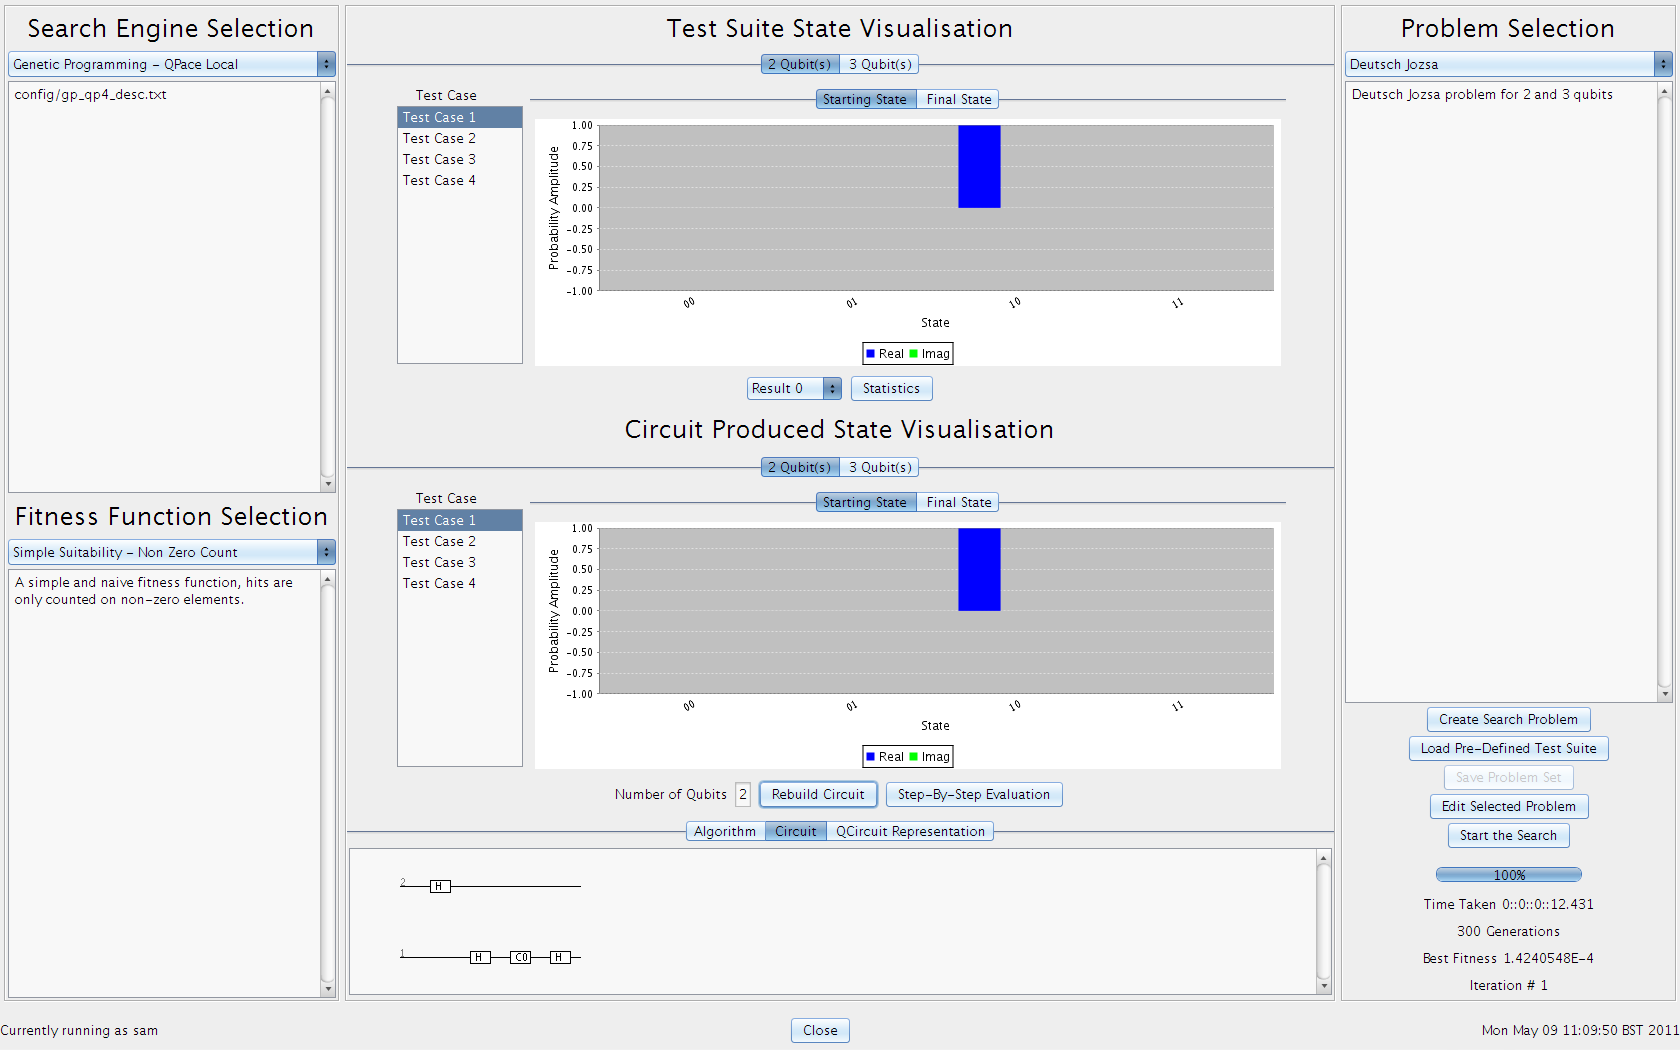
\includegraphics[width=\textwidth]{GUIDesign.png}
\caption{Main User Interface - After Search}
\label{fig:MainGUIDesign}
\end{figure}

Each section of the GUI is explained separately with reference to the principles listed.

\subsection{Main Window Layout}
As can be seen in Figure \ref{fig:MainGUIDesign} the layout of the main window separates the ``dissimilar things'' with the use of visible but subtle borders.
This meets the \emph{structure} principle.
The interface is structured so that the centre of the display contains the information of the highest importance, framed  by two control menus.
This central panel collates all of the main results of the latest search.
% The search statistics are shown in the right hand menu area.
% This separation ensures that the GUI does not become cluttered.

The layout is also intended to take into account the recent move towards wide screen monitors.
Wide screen monitors provide a new problem in GUI design.
If a GUI fills the screen area and fills it fully with the display of information, it can appear stretched and distorted.
If the GUI were to have a single menu along one side it also doesn't ``look right'', it looks excessively heavy on the non-menu side.
This is a issue with standard monitors also but in my opinion is exacerbated by the wide screen ratios.
Although it isn't directly related to any of the design principles it is an important property of a GUI to appear well balanced across the available screen area.

With the two menu panels the separation of the configuration options allows for a simple layout of configuration.
On the main window the only configuration that is available is the selection of the Search Engine, Suitability Measure and Search Problem.
The configuration of the Search Engine and the definition of the Search Problem is not handled by the main window.
This is to ensure that the display does not become overly cluttered, it maintains a simple and clean appearance.
This is a result of both the \emph{simplicity} and the \emph{visibility} principles.

\subsection{Search Engine, Suitability Measure and Search Problem Selection}
\label{sec:seselecdes}
\label{sec:smselecdes}
\label{sec:spselecdes}
Before a search can be started, selections have to be made for the Search Engine, Suitability Measure and Search Problem.
The selection of these are provided by three drop down lists.
The available options for a user to select are limited to the Search Engines and Suitability Measures that are registered in the respective managers in the framework.
For a user to add a new Search Engine or Suitability Measure the respective XML configuration file needs to be updated.
This was done so as to follow the \emph{simplicity} and \emph{tolerance} principles.
It ensures that any selection made by the user is a valid selection.

The selection of the Search Problem is again provided by a drop down list, following the \emph{simplicity} and \emph{tolerance} principles.
The difference is that the creation of a new problem from scratch and using a predefined test suite held in an XML file can be performed within the GUI.
Despite this difference, the use of the drop down list still ensures that any selection made by the user is a valid selection.
The validity of each individual Search Problem is checked by the editor dialogs described next.

All three of these selections are performed in the same way and ensure that the GUI maintains a level of consistency, meeting the \emph{reuse} principle.
When a selection is made, it is shown as selected and its description is displayed in the text area below, provided in the relevant configuration XML file, is shown.
The description areas are included to meet the \emph{feedback} principles and allow developers of Search Engines, Suitability Measures and indeed Search Problems to provide full text descriptions to the users from within the GUI.

\subsection{Search Problem Creator and Editor}
\label{sec:guisearchcreateed}
As mentioned above, the creation of Search Problems is provided by an on-screen dialog box.
The creation and editing of Search Problems is also provided by a standalone application, see Section \ref{sec:indtestsuiteeditor}.
The interface to includes an \emph{import from file} function.
This allows the user to register a new Search Problem using an XML file to define the test suite.
This allows researchers to easily register Search Problems created and distributed by other researchers.

The integrated editor and the standalone application use the same components and overall design.
The same components are also used when creating a new Search Problem and when editing an existing Search Problem.

Not only are the individual components reused but each dialog box follows the same design layout.
This promotes the \emph{reuse} and \emph{structure} principles.

The dialog boxes ensure that the user has entered values for the required fields and ensures that each entry is valid.
This implicitly ensures that each selection available to the user in the Search Problem drop down list is a valid option.
This follows the \emph{tolerance} principle.

\subsection{Reporting Results}
\label{sec:repres}

\begin{figure}
 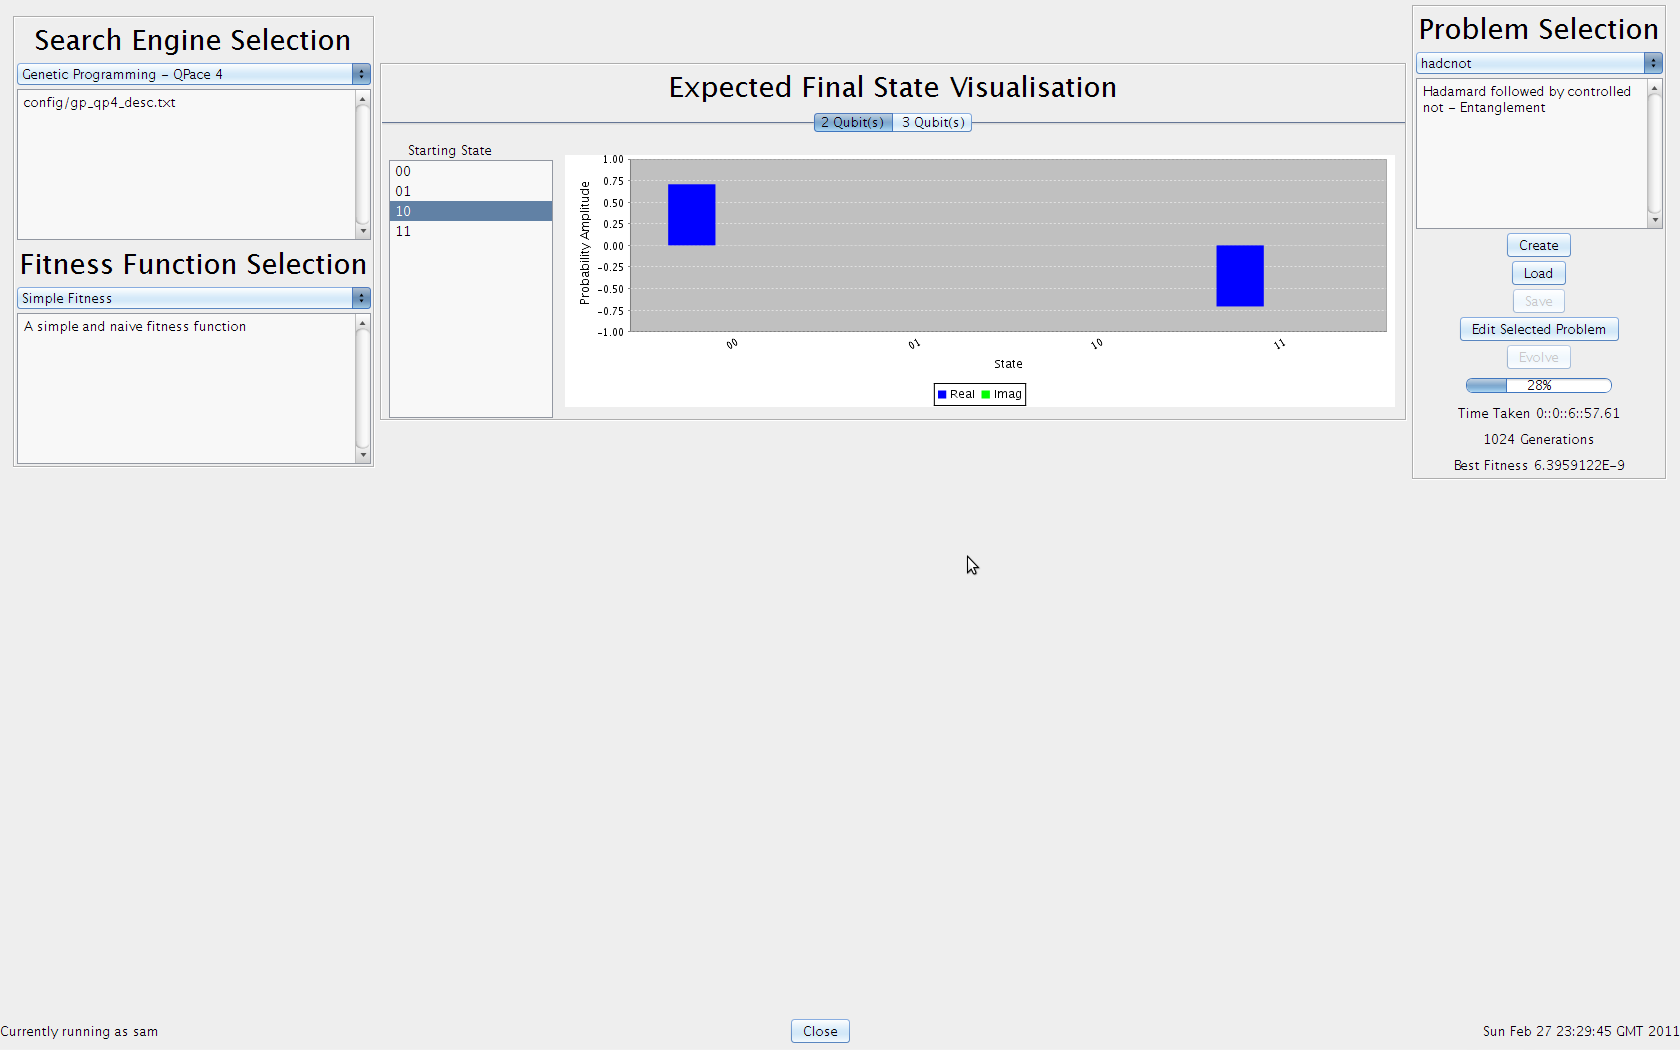
\includegraphics[width=\textwidth]{GUIDesignProgress.png}
\caption{Main User Interface - Before Search}
\label{fig:MainGUIDesignProg}
\end{figure}
\begin{figure}
 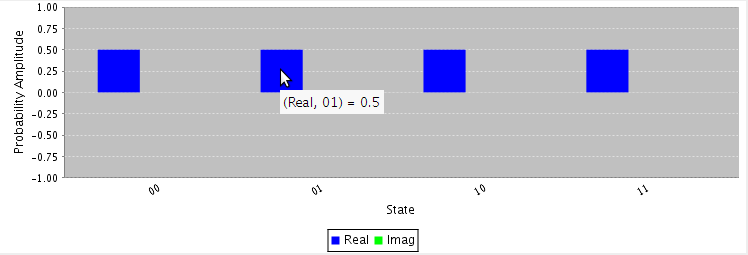
\includegraphics[width=\textwidth]{AccurateReadOutMouseOver.png}
\caption{Accurate State Readout}
\label{fig:AccStateReadOut}
\end{figure}
When a Search Problem is selected, in the central area a visual representation of the test suite is produced.
This representation can be seen in Figure \ref{fig:MainGUIDesignProg}.

After a search has been completed, the final states produced by the realised algorithm are shown using the same representation.
This can be seen in Figure \ref{fig:MainGUIDesign}.
Using a simple visualisation like this makes the comparison between ``desired'' final states and the final state produced by the algorithm found by the search.
It is true that the visualisation could be too simple for small differences to be noticed.
To counter this problem the visualisation allows the user to hover the mouse over each column to get an actual value.
This can be seen in Figure \ref{fig:AccStateReadOut}.

This provides users with both a quick, simple and visual way to compare final states as well as an accurate way to compare final states.
The accurate comparison method provided was implemented rather than a value table as part of following the \emph{simplicity} principle.

The result of a search is the quantum algorithm found by the search, rather than the final states for the test cases described so far.
The GUI provides the user 3 different ways to see the search result.
A simple textual listing of the algorithm is provided in the same format as the framework produces on its own.
To help with the users understanding of what the algorithm means a circuit diagram is produced for a user controlled number of Qubits.
The diagram is produced using the symbols that are shown in Table \ref{tab:providedgates}.
The circuits produced are not just provided as a circuit diagram but also in QCircuit representation so that the circuits can be placed into any publication produced in Latex simply with the use of the QCircuit package.

Providing the three representations meet the \emph{simplicity}, \emph{feedback} and \emph{reuse} principles.
The \emph{simplicity} principle is met as the result of the search is simplified to a human readable algorithm and circuits can be created to help the user understand how the algorithm is working.
The \emph{feedback} principle is met as the circuit diagrams that are produced are done so using widely accepted symbols and conventions for quantum circuit drawing.
The \emph{reuse} principle is met with the use of QCircuit to produce circuits in a form that can be included in publications.
An alternative would have been to output the circuit diagram that is drawn by the GUI as an image that could have been included in any, not just Latex, publication.
I feel the use of QCircuit is a better choice as the user then has control and is able to carry out, if necessary, manual circuit optimisation.

\subsection{Step-By-Step Evaluator}
\label{sec:sbse}

\begin{figure}
 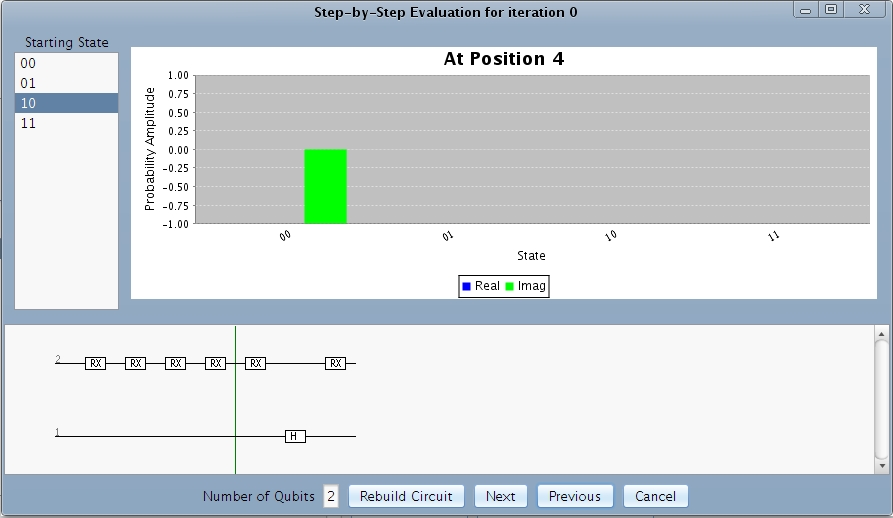
\includegraphics[width=\textwidth]{StepByStepEval.jpg}
\caption{Step-By-Step Evaluation Dialog}
\label{fig:StepByStepEval}
\end{figure}
The way in which quantum algorithms and the circuits they produce work is usually subtle and can be hard to understand by simply looking at the circuit.
The framework provides a step-by-step evaluation trace when provided with the input states.
The input states are provided to the framework in a test suite structure.
It was decided that the provided GUI would provide the test suite of the respective Search Problem.
This means that an evaluation trace is produced for each of the test cases, in each of the test suites.

The step-by-step evaluator is provided in a dialog box rather than integrated in the main frame.
This dialog box can be seen in Figure \ref{fig:StepByStepEval}.
This was done so as to focus the user's attention and to ensure that the addition of the functionality did not result in a cluttered GUI.
This follows the \emph{structure} and \emph{visibility} principles.

The step-by-step evaluation is performed with respect to a produced circuit.
This requires the user to select the number of qubits the circuit should be produced for and the step-by-step evaluation is provided for all test cases of that number of qubits.
Due to the design decision made for the framework, to provide a full trace rather than interactive evaluation, the test cases can be switched between at any step without returning to the start of the circuit.

The dialog box provides a circuit diagram, an initial state selector and a visual representation of the state at the ``current step'' in the evaluation for the selected initial state.
The circuit diagram is produced by reusing the circuit diagram drawn in the results pane of the main window.
This ensure that the circuit is represented using the same standards as that shown in the results pane.
The only difference is that the ``current step'' is indicated using a vertical line on the circuit diagram, this can be seen in Figure \ref{fig:StepByStepEval}.
This follows the \emph{reuse}, \emph{feedback},  \emph{visibility} and \emph{simplicity} principles.

The visual representation and initial state selector are the same as those used to report the final states produced for the test suite in the main window.
The only difference is that only the test cases for the current number of qubits is shown.
The use of the same visual representation ensure the user does not have to understand anything extra to use this functionality and follows the \emph{reuse} principle.

\section{Summary}

The design and implementation details outlined in the sections above cover all the functionality provided by the toolkit.
It is intended that the toolkit shall be released to the research community.
As a result the design and implementation was performed with a level of rigour that is possibly unusual for a student project.
Throughout the project third party libraries were employed to carry out specific tasks within the toolkit.
A full list of the libraries used can be found in Section \ref{sec:appsoftlibs}.
Libraries were used to reduce development risk and as part of the software engineering principles that were followed.

Both the design and implementation were produced following software engineering principles.
The extendibility of the toolkit has been kept central to the design.
The toolkit also focuses on the scalability provided.
With the representation of the circuit and algorithm using \emph{List} implementations the toolkit does not restrict the size of the algorithms or circuits that can be produced by the framework.
Additionally as the circuit evaluator progresses through circuits gate by gate rather than computing a matrix to represent the whole circuit this also is not adversely affected by the circuit size.
As is constantly referred to in the sections above the GUI of the client application was also designed in a principled manner.


The aims for the project remained constant throughout the process.
However, the ambition of the project increased quite frequently.
During weekly meetings additional functionality was frequently discussed and subsequently included in the toolkit.
To accommodate for the changing ambitions and the increasing functionality an agile approach was taken.
This proved very successful and the design was not compromised by the increases in functionality.
The implementation includes just under $13000$ lines of code implementing $751$ methods.
This is a large code base providing a high level of functionality.

Google CodePro\cite{codeproweb} was used to maintain a high level of quality over this large code base.
Using the core settings the code base was analysed and updated to address any violations found.
The type of issues found by CodePro were violations to coding conventions and good pactices.
For example exceptions were not originally logged by the framework when they were caught.
Subsequently Log4J\cite{log4jweb} has been used to implement this logging.
This shows another area where a more rigorous process has been used than would normally be expected in a student project.



% \subsubsection{The Structure Principle}
% As can be seen in Figure \ref{fig:MainGUIDesign} the layout separates the ``dissimilar things'' with the use of headings and borders.
% The interface can be viewed as structued so that the centre of the display contains the information of the highest importance, straffed by two control menus.
% This central panel collates all of the result information regarding the result of the latest search.
% The search statistics are shown in the right hand menu area.
% This separation ensures that the GUI does not become cluttered.
% 
% This layout is also intended to take into account the recent move towards wide screen monitors.
% Wide screen monitors provide a new problem in GUI design.
% If a GUI fills the screen area and fills it fully with the display of information, it can appear stretched and distorted.
% If the GUI were to have a single menu along one side it also doesn't look ``right'', it looks excessively heavy on the non-menu side.
% This is a issue with standard monitors also but in my opinion is excasserbated by the wide screen ratios.
% 
% As well as the main GUI, the dialogs used to Create, Load and Edit search problems are all structured in such a way so as to guide a user through the respective operation.
% 
% The implemented search engine also provides a dialog box to configure a series of parameters.
% This dialog is split into two sections.
% One section contains a selection of all available gates while the second provides a series of GP parameters that the user may be interested in configuring, such as the number of generation and the population size.
% This separation follows the structure principle and clearly separates to the two distinct sets of configuration options.
% 
% \subsubsection{The Simplicity Principle}
% The way in which the framework has been designed aids in making the user interface simple.
% The framework requires very little configuration.
% The only real configuration that is required is the selection of which search engine and suitability measure to use and what problem you want to try solve.
% These selections are provided in very simple drop down lists for the users seletion.
% 
% The GUI provides a visual way to Create new and Edit existing search problems.
% A standalone editor is also provided.
% The editor provides a 
% 
% The only other two aspects of the configuration are the problem editor and the configuration of the search parameters.
% These are justified separately.
% 
% \subsubsection{The Visibility Principle}
% I think it is quite clear to see that the number of ``options'' visible to the user at any one time is minimised.
% The use of drop down boxes for selection naturally hides unwanted options until required.
% 
% In the central area the available selections are visible but are also much more likely to be ``browsed'' by the user.
% The decision not to use drop down boxes for the initial state selection is due to the expected ``browsing'' of this data.
% I expect that the user is likely to flick through the various options available which is much easier when the options are always visible.
% The use of a drop down box would also have required two mouse clicks per selection, one to open the list and one to make the selection.
% With the options visible this is reduced to a single click.
% 
% \subsubsection{The Feedback Principle}
% Once a selection is made for any of the selections available to the user the information on the display is updated accordingly.
% For example, the selection of a different search engine will update the contents of the search engine description area, selecting a different ``input state'' in the graph panels automatically updates the graph and the selection is highlighted.
% 
% 
% The user interface has been designed so that one user could leave it, a second user come to use it and understand very quickly the decisions that had already been made.
% It is not just the selection choices that are provided to the user as feedback.
% As can be seen in Figure \ref{fig:MainGUIDesignProg}, a progress bar is provided to indicate to the user how far through the current search the system is.
% 
% \subsubsection{The Tolerance Principle}
% To meet the tolerance principle the user interface has been designed to ensure that any user input is either restricted to valid inputs or validated on acceptance, notifying the user of any invalid input.
% A good example of this is the way the user selects the Search Engine, Suitability Measure and Search Problem.
% These selections use drop-down lists.
% This ensures that, assuming a correct implementation, any selection made by the user is valid.
% 
% For user input that is not limited to a small finite set of inputs, all user inputs are checked on and any incorrect input is brought to the users attention.
% This tolerance ensures that the system allows the user to correct any problems without loosing any other input.
% 
% As is noted in Section \ref{sec:introtoquantcomp} all quantum gates must be unitary.
% To ensure the system complies with this, when creating custom matricies for custom gates, the editor checks the matrix to ensure that it represents a unitary operation.
% 
% 
% 
% \subsubsection{The Reuse Principle}
% 
% Visualisation of similar information is shown using the same techniques.
% The use of tabs is two-fold.
% In the column chart panels it is used to select the data to show using the chart.
% In the lowest panel it is used to switch between the different representations of the solution that the system provides.
% 
% 
% \begin{itemize}
%  \item Extendible Library
% \end{itemize}

% \chapter{Implementation}

\section{Framework}
\subsection{Complex Numbers}
Complex number representation is provided by class from http://www.math.ksu.edu/~bennett/jomacg/c.html.

\subsection{Matrices}

The Matrix representation is based on the Matrix class provided by the Jama library.
Jama Matrix is modified to provide Matricies of Complex numbers.
The extra funcitonality provided by Jama, such as eigendecomposition, has been disabled currently.

\subsection{Circuit in Latex Form}
Used QCircuit package

\subsection{Interactive Circuit Evaluator}

\section{Fully Implemented System}
\subsection{Quantum Gate Implemenation}


\subsection{Fitness Functions}

\subsubsection{Simple}

\subsubsection{Simple and Parsimony}

\subsubsection{Phase Aware}

\section{Provide GUI}
\subsection{Rendered Circuit Diagram}
Based on the code for JQuantum.


\subsection{Quantum Circuit Viewer}

\chapter{Testing}
\label{sec:testing}
\section{Unit Tests}
\label{sec:unittests}
Many of the components created for the framework were tested by unit testing.
With the framework created in Java, JUnit 4\cite{junitweb} was used to produce and run the unit tests.
Not all components were suitable for unit testing due to them being less functional and more control classes.
Therefore unit tests were not created for these components but they were tested as part of the integration testing.

The components that were tested are listed below:
\begin{itemize}
 \item Complex class
 \item Matrix class
 \item All gate implementations
 \item Circuit implementation
 \item Expnode implementation
 \item Algorithm implementation
 \item Suitability measures
 \item Manager classes
\end{itemize}

In the unit tests the test values were chosen in accordance with partition testing to ensure that the test were more complete and tested for the incorrect and the correct partitions with equal weight.

\subsection{Complex Number Implementation Unit Tests}
Due to the Complex class underpinning the functionality of the framework a thorough test was required; reliance on the testing performed on the third party library was to much of a risk.
The unit tests were simple with a range of positive, negative, integer and decimal values used in the construction of the complex classes.

The test oracles used for the \emph{toString} and \emph{parseComplex} methods were created in combination with the other of these two methods.
Additional test oracles were also used but this mutal dependance ensures that the strings produce by the \emph{toString} method are well formed and can be parsed by \emph{parseComplex}.
It also ensures that the \emph{parseComplex} method is correct and creates a Complex object that represents the string passed as its argument.

For the numeric methods, Octave\cite{octweb} was used to create test oracles.

\subsection{Matrix Implementation Unit Tests}
The Matrix is based on a third party implementation but due to both its importance to the correct operation of the framework and the extent of the modification made to it, extensive unit testing was performed.
Even though the framework only requires the correct operation of unitary matrices the testing was not restricted to unitary matrices.
Test matrices were created as real only,  imaginary only and real and imaginary complex values with both positive and negative values.

The Matrix unit tests include testing of the MatrixUtil class that provides the encoding and decoding of matrices to XML files and tensor product of two matrices.

For the arithmetic methods, Octave\cite{octweb} was used to create test oracles.

\subsection{Gate Implementation Unit Tests}
\label{sec:gatetests}
Unit testing the gate implementations is a relatively simple process.
The correct operation of the all gates, excluding the custom gates, are statically defined as in Table \ref{tab:providedgates}.
Therefore creating the unit tests are a series of tests to ensure that with predefined input states, the output states are correct with respect to the gate's definition.
To reduce the probability of errors being introduced into the test oracles used by the unit tests, the test oracles were calculated by Octave\cite{octweb} using Quantum Computing Functions(QCF) for Matlab\cite{qcfweb}.

QCF does not provide all of the gates defined in Table \ref{tab:providedgates}.
For the missing gates, Matlab functions were created using the definitions in Table \ref{tab:providedgates}.

To test the custom gate implementation XML files were created with the definitions of all single qubit gates.
Custom gates were created using these XML files and all the unit tests for the respective gate were applied.
This ensured that the operation of the custom gate is functionally equivalent to the non-custom gates.
The custom gate is not going to ne non-functionally equivalent as some of the non-custom gates exploit bit manipulation rather than matrix multiplication, see Section \ref{sec:custgates}, where as the custom gate can only perform matrix multiplication.

Alongside the \emph{apply} operation performed on quantum states, all other methods are also tested by the unit tests.
The test oracles are much simpler to define.
The \emph{getTarget} method is required to return the integer value set as the target qubit ID in the constructor.
A number of test cases including positive, negative and zero values.
Only positive values should be accepted by the constructor as there are no qubits with a negative or zero ID.
The returned value of each of the other operations are known either implicitly or explicitly by Table \ref{tab:providedgates} and the QCircuit\cite{QCsite} documentation.

\subsection{Circuit Implementation Unit Tests}
\label{sec:circtests}
The unit tests for the circuit implementation followed the following scenarios:
\begin{itemize}
 \item Add a gate
 \item Add a subcircuit
 \item Add a gate and ensure the Latex representation is correct
 \item Add a subcircuit and ensure the Latex representation is correct
 \item Add a gate and ensure the circuit size is correct
 \item Add a subcircuit and ensure the circuit size is correct
 \item Add a gate and ensure the gate in the iterator is correct
 \item Add a subcircuit and ensure the gates in the iterator are correct and in the correct order
\end{itemize}

\subsection{Expnode Implementation Unit Tests}
These unit tests concern the implementation of the Expnode context free grammar shown in Table \ref{tab:expnodecontext}.
The unit tests were based on the expressions that can be seen in Figure \ref{tab:expnodetestexps}.
A collection of values are used as SystemSize including positive, negative, integer and decimal values.
LoopVars shal also be set as one of a collection of arrays with lengths $0$, $1$, $2$ and $3$.
The $0$ length array is important as there is no restriction placed on the search engines stating that the loop variables can only be requested in a loop.
This is to that the search is not restricted.
If the array is of length $0$ the result is $0$ irrespective of the index requested.
If the index requested is greater than the length of the array, modulus is used with the array length to produce a valid index.
This is defined in Section \ref{sec:quantalgs}.

The test oracles are calculated in the test cases to ensure that precision rounding is handled by the test cases.

\begin{figure}
\centering
 \begin{tabular}{|c|c|c|c|}
\hline
$0$ & $2+SystemSize$ &  $LoopVars[0]$ &$2+LoopVars[2+SystemSize]$\\
$2$ & $2-SystemSize$ &   $LoopVars[1]$ & $2-LoopVars[2+SystemSize]$\\
$-2$ & $2*SystemSize$ &   $LoopVars[-1]$ & $2*LoopVars[2+SystemSize]$ \\
&$2/SystemSize$ &  $LoopVars[SystemSize]$ & $2/LoopVars[2+SystemSize]$ \\
&&  $LoopVars[2+SystemSize]$ & \\
\hline
 \end{tabular}
\caption{Expnode Test Expressions}
\label{tab:expnodetestexps}
\end{figure}

\subsection{Algorithm Implementation Unit Tests}
\label{sec:algtests}
The unit tests for the algorithm implementation followed the following scenarios:
\begin{itemize}
 \item Add an instruction
 \item Add four different instructions
 \item Add a instruction and ensure the algorithm size is correct
 \item Add four different instructions and ensure the algorithm size is correct
 \item Add a instruction and ensure the instruction in the iterator is correct
 \item Add four different instructions and ensure the instructions in the iterator are correct and in the correct order
 \item Add a instruction and ensure the printed algorithm is correct
 \item Add four different instructions and ensure the printed algorithm contains the correct instructions, including correct expressions to calculate the numeric vales, are correct and they are printed in the correct order
\end{itemize}

\subsection{Suitability Measure Unit Tests}
\label{sec:suitmeastests}
There are three suitability measures provided with the framework, see Section \ref{sec:provsuitmeas}.
Each of these needed to be tested to ensure that the implementation was consistent with their definitions.

A series of $2^n\times1$ matrices were created and provided to the suitability measure.
The theoretical value, the test oracle, was calculated using Oracle.
The matrices used in the testing were not necessarily correct quantum states, they may not have a modulus square equal to $1$.
This is because even though the operation of gates are by definition unitary, the starting state nor the expected final states defined in test cases are restricted to quantum states that have a modulus square equal to $1$.
As a result the suitability measure tests were not restricted to ``correct'' quantum states.

\subsection{Test Suite Unit Tests}
\label{sec:testsuitetests}
The test suite data structure is a combination of three classes not covered by other unit tests.
Although the test will cover three classes this is still being classed as a unit test as it is effectively a test of the data structure unit rather than the classes.

The tests covered the following scenarios:
\begin{itemize}
 \item (Three tests) Create a new test suite and insert a single test case for 1/2/3 qubits, check test suite data structure against the oracle.
 \item Create a new test suite and insert a single test case for 1 qubit and another test case for 2 qubits, check test suite data structure against the oracle.
 \item Create two new test suite (A and B), insert a single test case for 1 qubit in test suite A and 1 qubit in test suite B, add the test set from test suite B to test suite A. Check test suite A and B data structures against the oracles.
 \item Create a new test suite and insert a single test case for 1 qubit and another test case for 2 qubits, encode the test suite as an XML file, check the test suite XML file against the oracle.
 \item Decode a predefined test suite XML file, check the test suite data structure against the oracle.
\end{itemize}

The scenario consisting of two test suites checks both test suites to ensure that the merge of test sets, and therefore the modification of labels and IDs, does not effect the test suite that is not being modified.

\subsection{Manager Classes Unit Tests}
\label{sec:manclasstests}
For each of the manager classes, a series of XML configuration files were created for testing purposes only.
For the Search Engine and Suitability Measure Manager classes the tests contained several checks:
\begin{itemize}
 \item Check the list of available implementations against the oracle
 \item Select each implementation in turn and check against the oracle the class of the object provided by the manager
\end{itemize}

For the Problem Manager the checks were slightly more in depth due to the returned object containing a test suite data structure.
The test suite implementation includes an \emph{equal} method which provides a ``deep equality'' check.
This is used by the unit test to ensure that the object created by the manager against an oracle.

\section{Integration Tests}
As mentioned in Section \ref{sec:unittests}, the framework contains classes that coordinate the interaction between the functional classes.
The integration tests were designed to test these classes in particular.
These classes in particular were:
\begin{enumerate}
 \item The circuit builder implementation - \emph{basiccircuitbuilder}
 \item The circuit evaluator implementation - \emph{basiccircuitevaluator}
\end{enumerate}

The approach that was taken was a bottom-up approach.
The tests were also performed in the order they are listed.
This is becuase the circuit builder is used by the circuit evaluator and therefore it imposes a dependency.

\subsection{Circuit Builder Integration Tests}
The circuit builder integration test combined:
\begin{itemize}
 \item Gate implementations
 \item Circuit implementation
 \item Algorithm implementation
\end{itemize}

Due to the simplicity of the circuit builder interface, the tests that were carried out were also simple.
The circuit builder interface provides two methods.
Both methods are intended to perform the same action, to take a quantum algorithm and to return the circuit for the specified system size.
The difference between the two methods is that one allows an integer array to be passed as an argument.
This integer array is the \emph{LoopVars} array used in the Expnode grammar, see Section \ref{sec:quantalgs}.
When the method without this argument initialises the \emph{LoopVars} array to the empty array.

To test the two methods, a collection of simple quantum algorithms were produced to include each gate instruction at least one and each of the iterate control instructions at least five times.
These algorithms are passed to the circuit builder, the returned circuits are checked against the test oracles.
The test oracles are circuits that represent the circuit that would be created by the algorithm.

The tests are run over system sizes of 1, 2 and 3.
Using a code review, the method with the additional integer array parameter will be tested by the other method when the algorithm includes iterate control instructions.
This is the reason which each gate was included at a minimum of once but the iterate control instruction were included at least five times.

\subsection{Circuit Evaluator Integration Tests}
\label{sec:cirevaltests}
The circuit evaluator integration test combined:
\begin{itemize}
 \item Circuit builder implementation
 \item Suitability measure implementation
 \item Test suite implementation
\end{itemize}

The suitability measure that was used for the tests was the Simple Suitability Measure, see Section \ref{sec:simplsuitmeas}.

The tests for the circuit evaluator were very similar to those used to test the individual suitability measures, see Section \ref{sec:suitmeastests}.
A series of algorithms were produced alongside a collection of small test suites, containing less that three test cases.
The theoretical suitability value of each algorithm was produced and then compared with the value produced by the circuit evaluator.

Two additional tests were produced to test the \emph{getResults} and \emph{getTrace} methods.
The test oracles were test suites and arrays of test suites respectively.
To ensure that the tests were simple enough that confidence was improved in the test oracle structures that had to be produced manually.
The quantum states in the test oracles that represented the result of correct complete or partial circuit evaluation were produced using Octave also to improve test confidence.

\section{System Testing}
\label{sec:systests}

\section{Client GUI Testing}
\label{sec:clientguitests}
The client GUI that is provided alongside the framework was tested using scenario based testing.
For each of the requirements for the client GUI, see Section \ref{sec:clientguireqs}, had a scenario created specifically for the requirement.

Analysing all the test cases produced, many could be combined producing a much smaller number of test cases without reducing the requirement coverage.
The test cases were analysed for a second time to identify those that could be automated.
The tool chosen for the automated was WindowTester Pro\cite{wintestproweb}.
However, it was decided that the amount of automation that was possible and the limitations of what could be checked during the automated tests did not make it a sensible to proceed with automation of the GUI testing.

\clearpage
\begin{landscape}
\section{Tracability}
\label{sec:tracability}

\centering
\noindent\begin{longtable}{|c|m{10cm}|c|m{3cm}|m{3cm}|}
\hline
\textbf{Requirement ID} &
\multicolumn{1}{c|}{\textbf{Requirement Title}} &
\textbf{Full Requirement} &
\textbf{Addressed by Design} &
\multicolumn{1}{c|}{\textbf{Addressed by Test}} \\ \hline

Req:ASE &
The framework shall allow researchers to provide search engines for the system to use. &
Page \pageref{sec:reqase} &
Section \ref{sec:mulsearchen} &
\multicolumn{1}{c|}{Section \ref{sec:manclasstests}}\\ \hline

Req:ASM &
The framework shall allow researchers to provide suitability measures for the system to use. &
Page \pageref{sec:reqasm} &
Section \ref{sec:mulsuitmeas} &
\multicolumn{1}{c|}{Section \ref{sec:manclasstests}}\\ \hline

Req:QAO &
The solution of a search, a quantum algorithm, shall be presented to the user as a list of instructions. &
Page \pageref{sec:reqqao} &
Section \ref{sec:quantalgs} &
\multicolumn{1}{c|}{Section \ref{sec:algtests}} \\ \hline

Req:CV &
The system shall provide visualisation of the circuit produced by the solution of the search for a system of a user specified number of qubits. &
Page \pageref{sec:reqcv} &
Section \ref{sec:quantumcircuits} &
\multicolumn{1}{c|}{Section \ref{sec:circtests}} \\ \hline

Req:TPS &
The framework shall be able to be embedded in third party software. &
Page \pageref{sec:reqtps} &
Section \ref{sec:thirdpartyblackbox} &
Code Review of Client to ensure only interface knowledge is required\\ \hline

Req:DST &
The framework shall provide a standardised definition format for users to specify the target of the search. &
Page \pageref{sec:reqdst} &
Section \ref{sec:testsuitestruc} &
\multicolumn{1}{c|}{Section \ref{sec:testsuitetests}} \\ \hline

Req:UCF &
The customisation of the framework shall be provided through a series of configuration files. &
Page \pageref{sec:requcf} &
Section \ref{sec:manclasses} &
\multicolumn{1}{c|}{Section \ref{sec:manclasstests}} \\ \hline

Req:PGAI &
The framework shall provide implementations of all gates specified in Table \ref{tab:providedgates}. The framework shall provide algorithm instructions for each of these gates and for the instantiation of the Controlled-U gate with all single qubit gates. &
Page \pageref{sec:reqpgai} &
Sections \ref{sec:quantalgs}, \ref{sec:quantumgates} &
\multicolumn{1}{c|}{Sections \ref{sec:gatetests}, \ref{sec:algtests}} \\ \hline

Req:ACS &
The system shall provide the iterate control structure and support nested iterate instructions. &
Page \pageref{sec:reqacs} &
Section \ref{sec:quantalgs} &
\multicolumn{1}{c|}{Sections \ref{sec:gatetests}, \ref{sec:algtests}} \\ \hline

Req:PCA &
The framework shall be able to produce a circuit, for any given number of qubits, from a quantum algorithm. &
Page \pageref{sec:reqpca} &
Sections \ref{sec:quantumcircuits}, \ref{sec:quantumgates} &
Code review of both the circuit implementation and all of the gate implementations to ensure the logic does not rely on upper bound to the system size.
The only restriction that is present is where $2^{System Size}>Integer.MAX\_VALUE$. \\ \hline

Req:CS &
The framework shall provide the simulation of a circuit given an initial state. &
Page \pageref{sec:reqcs} &
Section \ref{sec:quantumgates} &
\multicolumn{1}{c|}{Sections \ref{sec:gatetests}, \ref{sec:cirevaltests}} \\ \hline

Req:SBSSE &
The framework shall provide a way to perform step-by-step evaluation of a circuit given an initial state. &
Page \pageref{sec:reqsbsse} &
Section \ref{sec:sbsecireval} &
\multicolumn{1}{c|}{Section \ref{sec:cirevaltests}} \\ \hline

&&&&
\\ \hline

Req:SSE &
The tool shall provide at least one implemented search engine. &
Page \pageref{sec:reqsse} &
Section \ref{sec:provsearcheng} &
\multicolumn{1}{c|}{Section \ref{sec:manclasstests}} \\ \hline

Req:SSM &
The tool shall provide at least one implemented suitability measure. &
Page \pageref{sec:reqssm} &
Section \ref{sec:provsuitmeas} &
\multicolumn{1}{c|}{Section \ref{sec:manclasstests}} \\ \hline

Req:SST &
The tool shall provide a number of search targets with known outputs. &
Page \pageref{sec:reqsst} &
Section \ref{sec:provsearchprobs} &
\multicolumn{1}{c|}{Section \ref{sec:manclasstests}} \\ \hline

Req:SES &
The GUI shall provide a user with a selection of search engines to use in a search. &
Page \pageref{sec:reqses} &
Section \ref{sec:seselecdes} &
\multicolumn{1}{c|}{Section \ref{sec:clientguitests}} \\ \hline

Req:SMS &
The GUI shall provide a user with a selection of suitability measures to use in a search. &
Page \pageref{sec:reqsms} &
Section \ref{sec:smselecdes} &
\multicolumn{1}{c|}{Section \ref{sec:clientguitests}} \\ \hline

Req:STS &
The GUI shall provide a user with a selection of search targets to be used as the search goal. &
Page \pageref{sec:reqsts} &
Section \ref{sec:spselecdes} &
\multicolumn{1}{c|}{Section \ref{sec:clientguitests}} \\ \hline

Req:STC &
The GUI shall provide a way for users to create a new search target without needing to explicitly write a configuration file. &
Page \pageref{sec:reqstc} &
Section \ref{sec:guisearchcreateed} &
\multicolumn{1}{c|}{Section \ref{sec:clientguitests}} \\ \hline

Req:STE &
The GUI shall provide a way for users to edit the contents of a previously created search target without manual editing of the configuration file. &
Page \pageref{sec:reqste} &
Sections \ref{sec:indtestsuiteeditor}, \ref{sec:guisearchcreateed} &
\multicolumn{1}{c|}{Section \ref{sec:clientguitests}} \\ \hline

Req:LSTPDC &
The GUI shall provide a way to import a predefined search target from a configuration file. &
Page \pageref{sec:reqlstpdc} &
Section \ref{sec:guisearchcreateed} &
\multicolumn{1}{c|}{Section \ref{sec:clientguitests}} \\ \hline

Req:SV &
The GUI shall provide a way to visualise any quantum state. &
Page \pageref{sec:reqsv} &
Section \ref{sec:repres} &
\multicolumn{1}{c|}{Section \ref{sec:clientguitests}} \\ \hline

Req:RSR &
The GUI shall provide a way to report the search result, a quantum algorithm, to the user. &
Page \pageref{sec:reqrsr} &
Section \ref{sec:repres} &
\multicolumn{1}{c|}{Section \ref{sec:clientguitests}} \\ \hline

Req:GCV &
Given a quantum algorithm and a system size, the GUI shall produce a visualisation of the resulting circuit. &
Page \pageref{sec:reqgcv} &
Section \ref{sec:repres} &
\multicolumn{1}{c|}{Section \ref{sec:clientguitests}} \\ \hline

Req:GSBSSE &
The GUI shall provide a way to perform, control and visualise the step-by-step state evolution for an intial state and circuit. &
Page \pageref{sec:reqgsbsse} &
Section \ref{sec:repres} &
\multicolumn{1}{c|}{Section \ref{sec:clientguitests}} \\ \hline

Req:TT &
The GUI shall provide user help through the use of tooltips. &
Page \pageref{sec:reqtt} &
Implemented for all buttons&
\multicolumn{1}{c|}{Witnessed during Section \ref{sec:clientguitests}} \\ \hline

Req:POR &
The framework, fully implemented tool and the GUI shall be able to be used on a range of Operating Systems. &
Page \pageref{sec:reqpor} &
Property of Java, Section \ref{sec:reqs} &
\multicolumn{1}{c|}{Section \ref{sec:clientguitests}} \\ \hline

\end{longtable}
\end{landscape}
\clearpage

\chapter{Experimentation}
\label{sec:experimentation}

The majority of this report concentrates on the details of the design of the toolkit and however so far no experimentation has been performed using the implemented toolkit.
This section is soley focused on using the toolkit in a series of experiments aimed at solving a selection of previously solved quantum problems.

\section{Deutsch Algorithm}
\label{sec:deutschexperiment}
The details of the Deutsch algorithm is presented in Section \ref{sec:DeutAlg}.
The problem is to determine whether the binary function $f$ is balanced or constant.
The Deutsch algorithm only applies to functions $f$ with a single input qubit.
Each of the four possible binary functions are either balanced or constant.

This search problem uses the toolkit's custom gate mechanism to define the four test cases, one for each of the possible binary functions.
The problem is provided with a single ancillary qubit resulting in a system size of $2$ qubits.
The input state for each test case is $\ket{10}$.

Using this input state could be seen as cheating slightly as the solution is hinted at by the input state.
However, analysing the solutions to similar quantum problems, such as the Deutsch-Jozsa or even the one out of four algorithm, it is the input state $\ket{10}$ is a sensible suggestion.

\begin{figure}
\centering
\subfigure[$f_1$]{
$
\begin{pmatrix}
1 & 0 & 0 & 0 \\
0 & 1 & 0 & 0 \\
0 & 0 & 1 & 0 \\
0 & 0 & 0 & 1 
\end{pmatrix}
$
}
\subfigure[$f_2$]{
$
\begin{pmatrix}
0 && 0 && 1 && 0 \\
0 && 0 && 0 && 1 \\
1 && 0 && 0 && 0 \\
0 && 1 && 0 && 0 
\end{pmatrix}
$
}
\subfigure[$f_3$]{
$
\begin{pmatrix}
1 && 0 && 0 && 0 \\
0 && 0 && 0 && 1 \\
0 && 0 && 1 && 0 \\
0 && 1 && 0 && 0 
\end{pmatrix}
$
}
\subfigure[$f_4$]{
$
\begin{pmatrix}
0 && 0 && 1 && 0 \\
0 && 1 && 0 && 0 \\
1 && 0 && 0 && 0 \\
0 && 0 && 0 && 1 
\end{pmatrix}
$
}
\caption{Matrices of Custom Gates Implementing the four Possible Functions}
 \label{fig:deutschfunctions}
\end{figure}

\begin{figure}
\[
\Qcircuit @C=1.0em @R=.7em {
 & \targ & \qw \\
 & \gate{\mathcal{F}}\qwx & \qw
}
\]
\caption{Matrix Circuit}
 \label{fig:matrepresentation}
\end{figure}


Custom gates are used to provide the oracle functions.
The matrices implementing the oracles can be seen in Figure \ref{fig:deutschfunctions}.
The matrices are the two qubit unitary operations of a controlled not acting on the more significant qubit.
However, the control is not provided by the value of the lower significant qubit, $x$, but the value $f(x)$.
They effectively represent the circuit shown in Figure \ref{fig:matrepresentation}.
It can be seen that the circuit of the Deutsch Algorithm, Figure \ref{Deutsch-Cir}, includes the circuit represented by the matrices.
The circuit in Figure \ref{fig:matrepresentation} is inverted due to the numbering of the qubit identifiers and significance in the framework.
The matrices have been created taking into account the different qubit numbering so the semantics of the circuit in Figure \ref{fig:matrepresentation} and the respective section of the Deutsch Algorithm circuit in Figure \ref{Deutsch-Cir} are the same.

The start state for each test case is $\ket{10}$.
For functions $1$ and $2$, which are constant, the expected final state is $\frac{1}{\sqrt{2}}(\ket{00}-\ket{10})$, equivalent to $\frac{1}{\sqrt{2}}((\ket{0}-\ket{1})\ket{0})$.
For functions $3$ and $4$, which are balanced, the expected final state is $\frac{1}{\sqrt{2}}(\ket{01}-\ket{11})$, equivalent to $\frac{1}{\sqrt{2}}((\ket{0}-\ket{1})\ket{1})$
It is simple to see that, taking into account the different qubit numbering, these are the same output states that are produced by the Deutsch Algorithm in Section \ref{sec:DeutAlg}.

After creating the custom matrices using the provided matrix editor, see Section \ref{sec:indmatrixeditor}, and the test suite using the integrated search problem creator, all elements required for the search were complete.
The search engine that was used was the genetic programming search engine, using local threads rather than the JPPF distribution, provided by the prototype implementation, see Section \ref{sec:provsearcheng}.
The suitability measure that was used was the Simple suitability measure variant that only reports a ``hit'' for non-zero expected values, see Section \ref{sec:simplsuitmeas}.

All instructions were included in the search except \emph{Create\_SWAP} and \emph{Create\_Zero}.
The default search parameters except time was not used to produce the seeds to ensure repeatability.

The full algorithm that was proffered as the final solution is listed in Section \ref{sec:DeutschExpAppFullAlg}.
The algorithm below is a hand optimised version of that listed in \ref{sec:DeutschExpAppFullAlg} with only the instructions that apply when \emph{System\_Size} is $2$.

\begin{lstlisting}
Create_H on gate 0
Create_H on gate 1
Create_Custom1 on gate 1
Create_H on gate 1
\end{lstlisting}

The first instruction is to put a Hadamard gate onto gate $0$.
Gate zero doesn't exist as the qubit numbering is from $1$ upwards.
This is an example of when the genetic programming has taken advantage of the environment.
$0$ is used as the value for the ``System\_Size'' flag within the system.
When an expression tree evaluates to $0$ it is effectively instructing that it should be replaced by the system's size.

The circuit produced by this algorithm is shown in Figure \ref{fig:evodeutschcir}.
The gate \emph{C0} is ``custom gate 1'' provided by the test cases, i.e. the custom unitary operations defined in Figure \ref{fig:deutschfunctions}.

\begin{figure}
\[
\Qcircuit @C=1.0em @R=.7em {
&\gate{H}&\qw&\multigate{1}{C0}&\qw&\\%2
&\qw&\gate{H}&\ghost{C0}&\gate{H}&\\%1
}
\]
\caption{Circuit Produced by Algorithm for Two Qubits}
\label{fig:evodeutschcir}
\end{figure}

It is obvious that the search process has found the exact same circuit that was published by Cleve et al\cite{Cleve98quantumalgorithms} and is a deterministic solution.
This is an unprecedented result.
To the best of my knowledge, this circuit has not been produced using heuristic search by previous research.
This is also, to the best of my knowledge, the first time a deterministic algorithm has been found, using heuristic search, for the original Deutsch, single input qubit oracles, problem.

\section{Deutsch-Jozsa Problem}
\label{sec:deutschjozsaexperiment}

After success with the original Deutsch problem the most natural progression is to multiple qubit Deutsch-Josza problem.
The basic aim is the same, to decide if a function is balanced or constant.
However, unlike when the input cardinality is $1$ there exist functions with input cardinality $n$ that are neither balanced or constant.
The Deutsch-Jozsa algorithm only applies when $f$ is guaranteed to be either balanced or constant.

In this experiment, the test suite used includes the test cases with oracle functions on $1$ and $2$ qubits.
There are twelve test cases for the Deutsch-Jozsa algorithm.
$6$ balanced two qubit function, $2$ constant two qubit functions, $2$ balanced single qubit functions and $2$ constant single qubit functions.
After conducting the previous experiment, genetic programming is known to produce a solution to the single qubit problem and it is expected that including these test cases will assist the search for a more general solution.

Custom matrices were made to represent the oracle functions.
The matrices for the $2$ qubit oracles are shown in Figure \ref{fig:deutschjozsafunctions} of Section \ref{sec:deutschjozsa}.

The same test cases as used in the previous experiment is used as the single qubit test set.
For the two qubit oracles, the test cases that are used all have a staring state of $\ket{100}$.
For $f_1$ and $f_2$ the expected final state is set to $\frac{1}{\sqrt{2}}(\ket{000}-\ket{100})$.
For $f_3$, $f_4$ ,$f_5$, $f_6$, $f_7$ and $f_8$ the expected final state is set to $\frac{1}{\sqrt{6}}(\ket{001}+\ket{010}+\ket{011}-\ket{101}-\ket{110}-\ket{111})$.

The search engine that was used was the genetic programming search engine provided by the prototype implementation, see Section \ref{sec:provsearcheng}.
The suitability measure that was used was the Simple suitability measure variant that only reports a ``hit'' for non-zero expected values.

Initial experimentation showed that this search problem was significantly harder than the previous experiment.
All instructions were included in the search except \emph{Create\_SWAP}, \emph{Create\_Zero} and \emph{RevIterate}.
The final search parameters used are shown in Figure \ref{fig:deutschjozsaparams} in Section \ref{sec:deutschjozsasearchparams}.
The time was not used as the seeds so this experiment is reproducible.

The full algorithm that was found is listed in Section \ref{sec:DeutschJozsaExpAppFullAlg}.
Algorithm \ref{alg:deutjozsatwoqubits} is a hand optimised version of that listed in \ref{sec:DeutschExpAppFullAlg} with only the instructions that apply when \emph{System\_Size} is $2$.
Instructions marked by an asterisk refer to gates that have been removed from the hand optimised two qubit circuit shown in Figure \ref{fig:deutjoz2qubits}.
As the experssions have been evaluated with \emph{System\_Size}$==2$ it is a program rather than an algorithm.

% \lstset{numbers=left,language=Java, breaklines=true}
\begin{algorithm}
 \begin{algorithmic}
\STATE Create\_H on gate 1.0 *
\STATE Create\_H on gate 1.0 *
\STATE Create\_H on gate System\_Size
\STATE Create\_H on gate System\_Size *
\STATE Create\_H on gate System\_Size *
\STATE Create\_CCustom1 on gate 1.0 and gate 2.0
\STATE Create\_H on gate 1.0
\STATE Create\_H on gate System\_Size *
\STATE Create\_H on gate System\_Size *
\STATE Create\_CCustom1 on gate 1.0 and gate 2.0
\STATE Create\_H on gate 1.0
 \end{algorithmic}
\caption{Program to Produce the Solution for the Two Qubit Deutsch-Jozsa Problem}
\label{alg:deutjozsatwoqubits}
\end{algorithm}

% \begin{lstlisting}
% Create_H on gate 1.0 *
% Create_H on gate 1.0 *
% Create_H on gate System_Size
% Create_H on gate System_Size *
% Create_H on gate System_Size *
% Create_CCustom1 on gate 1.0 and gate 2.0
% Create_H on gate 1.0
% Create_H on gate System_Size *
% Create_H on gate System_Size *
% Create_CCustom1 on gate 1.0 and gate 2.0
% Create_H on gate 1.0
% \end{lstlisting}

Figures \ref{fig:deutjoz2qubits} and \ref{fig:deutjoz3qubits} show hand optimised versions of the circuit the produced by the algorithm for two and three qubits respectively.
The full circuits that have not been optimised are shown in Section \ref{sec:DeutschJozsaExpAppFullCirs}.
The gate \emph{C0} is ``custom gate 1'' provided by the test cases, i.e. the custom unitary operations defined in Figures \ref{fig:deutschfunctions} and \ref{fig:deutschjozsafunctions}.
The \emph{C0} gate rendering has also been modified to take into account the knowledge of gate size that the framework cannot assume when producing the QCircuit representation.
The full circuits in Section \ref{sec:DeutschJozsaExpAppFullCirs} are exactly as the framework produced them and do not show the actual gate size.
The controls shown in the circuits of Section \ref{sec:DeutschJozsaExpAppFullCirs} are also removed as they cannot be on a qubit affected by \emph{C0}, see Section \ref{sec:quantumgates}.

\begin{figure}
\centering
\subfigure[Two Qubits]{
$
\Qcircuit @C=1.0em @R=.7em {
%&3			&6					&7			&10					&11	&\\
&\gate{H}	&\multigate{1}{C0}	&\qw		&\multigate{1}{C0}	&\qw&\qw&\\%2
&\qw		&\ghost{C0}			&\gate{H}	&\ghost{C0}			&\gate{H}&\qw&\\%1
}
$
\label{fig:deutjoz2qubits}}
\subfigure[Three Qubits]{
$
\Qcircuit @C=1.0em @R=.7em {
% &1			&2			&3					&4			&5			&6					&7&\\
&\gate{H}	&\qw		&\multigate{2}{C0}	&\qw		&\qw		&\multigate{2}{C0}	&\qw&\qw&\\%3
&\qw		&\gate{H}	&\ghost{C0} 			&\qw		&\gate{H}	&\ghost{C0} 			&\qw&\qw&\\%2
&\qw		&\qw		&\ghost{C0}			&\gate{H}	&\qw		&\ghost{C0}			&\gate{H}&\qw&\\%1
}
$
% \caption{Deutsch-Jozsa Solution - Three Qubits - Hand Optimised}
\label{fig:deutjoz3qubits}}
\caption{Deutsch-Jozsa Solutions}
\end{figure}

Even the hand optimised circuits are not optimal, they contain more calls to the oracle, the \emph{C0} gates, compared to the standard Deutsch-Jozsa circuits, Figure \ref{Deutsch-Jozsa-Cir}.
The Deutsch-Jozsa circuit only use a single call to oracle whereas the circuits in Figures \ref{fig:deutjoz2qubits} and \ref{fig:deutjoz3qubits} make two calls.
The previous attempt made by Spector \emph{et al.}\cite{LSpectorGPforQC,LSpectorANDOR,Spector:1999:QCA:316573.317112} only used a single call to the oracle.
However, Spector \emph{et al.} placed that restriction on the search and were only searching for the circuit for the 3 qubit problem.
Due to the use of the standard circuit builder provided by the framework, the restriction was not placed on the search process.
The solution found by Spector \emph{et al.} was also only probabilistic whereas the solutions provided here are deterministic.

Even though the circuits use two calls to the oracle, it is it could be possible to manually transform the circuits produced to use a single oracle call.
% % % Even though the circuits show that the \emph{C0} gate is controlled, it is not.
% % % This is because the \emph{C0} gate covers three gates.
% % % However, due to the flexible nature of the custom gates, when the QCircuit encoding is produced the gate size is unknown so is shown as though it were a single qubit gate.
% % % When a controlled gate is constructed by the circuit builder, the control is only applied if it is not a qubit that would be acted on by the gate under control.
% % % If the qubit would be acted on, the effect of the control is removed, see Section \ref{sec:quantumgates}.

% In Figures \ref{fig:deutjoz3qubits} the gates are numbered.
% It can be reasoned that gate $4$ and $5$ can be swapped due to the matrix equivalent to applying gate $4$ followed by gate $5$ is the same as the matrix equivalent to applying gate $5$ followed by gate $4$.
% This would produce two similar portions of the circuit, gates $2$, $3$ and $5$, and gates $4$, $6$ and $7$.


\section{Quantum Fourier Transform}

The most impressive result presented in Massey's thesis\cite{masseythesis} and subject of the subsequent paper\cite{Massey:2005:EHQ:1068009.1068288} was the evolution of an algorithm to produce the Quantum Fourier Transform(QFT).
With the QFT acting as such a central part of Shor's Algorithm, see Section \ref{sec:shorsalg}, it is a very important element for quantum algorithms.

To try reproduce the results found by Massey, the test cases for QFT acting on two and three qubits were initially used.
These were created using Octave\cite{octweb} using Quantum Computing Functions(QCF) for Matlab\cite{qcfweb}.
The input states that were used were all twelve possible non-superpositional states.
All test states are provided in Section \ref{sec:quantfourtransexp}.


The search engine that was used was the Q-Pace based search engine provided with the framework, see Section \ref{sec:provsearcheng}.
The suitability measure that was used was the Phase sensitive suitability measure, see Section \ref{sec:phaseawaresuitmeas}.
The final search parameters used are shown in Figures \ref{fig:qftparams} and \ref{fig:qftgates} in Section \ref{sec:qftsearchparams}.

\section{0..3 Permutation Max Problem}
\label{sec:maxproblemexp}

The $0..3$ permutation problem is used by Massey\cite{masseythesis} to evaluate Q-PACE III.
The problem is quite simple, given a permutation of the numbers $0..3$ give the index of the maximum value, $3$.
Due to the simplicity of the problem it was chosen for the user guide produced for the client provided with the framework, see Section \ref{sec:userguide}.

Interestingly a deterministic solution was not found by Massey for all $24$ possible permutations.
Only a probabilistic solution was discovered.
This is the first experiment where a probabilistic solution is expected.
Massey specifically searched for a probalistic solution with a fitness function designed as such.

The search engine that was used was the genetic programming search engine provided by the prototype implementation, see Section \ref{sec:provsearcheng}.
Initially, the suitability measure that was used was the basic Simple suitability measure variant.

All instructions were included in the search except \emph{Create\_SWAP}, \emph{Create\_Zero} and \emph{RevIterate}.
% These were removed when the search was not making progress.
The search parameters were the defaults except the mutation rate was set to $0.003846154$, $\frac{0.1}{26}$, and time was not used as the seeds so this experiment is reproducible.

Initial results were disappointing and provided little useful information.
The solution that is presented by Massey includes the use of the Controlled-Controlled-Not(CCN) gate that is not included in the requirements and therefore could not be produced by the framework.
The decision was made to extend the framework past the original requirements and include the CCN gate.
To reduce the impact on the existing framework, the gate was implemented as a Controlled-U gate where U was a controlled-PauliX gate.
The CCN gate obviously requires 3 qubits identifiers, the third qubit identifier was provided by casting the phase value to an integer.
The addition of the CCN gate required additional logic to ensure the control qubits were set with the control qubit closest to the target qubit set as the control qubit of the inner Controlled-PauliX gate.
This is necessary for the matrix calculation.
If this logic were not performed the matrix calculated could be incorrect as the control of the outer Controlled-U gate would have to be inserted into the matrix of the inner Controlled-PauliX gate rather than the other way round.

Even with the addition of the CCN gate the results were not that impressive.
A different approach was taken to try and improve the results.
Reflecting on the difficulties encountered when specifying the desired output state the Zero Focussed variant of the Simple suitability measure was developed.
The difficulties encountered and the Zero Focussed variant are described fully in Section \ref{sec:simplsuitmeas}.
With the new suitability measure implemented the results were astounding.

Algorithm \ref{alg:03permalg} was proffered as the solution.
The circuit produced when \emph{System\_Size} is $4$ is shown in Figure \ref{fig:03circuitsolalg}.
This circuit contains the gate 
$
\Qcircuit @C=1.0em @R=.7em {&\gate{X T 4}&\qw&\\&\ctrl{-1}&\qw}
$
which represents the CCN gate.
The symbols inside this gate indicate certain properties of the CCN gate.
The $X$ symbol indicates that the operation under control is the Pauli-X gate.
The $T 4$ shows that the target of the CCN is qubit $4$ that means that qubit $2$, the qubit on which the gate is shown, is a control qubit.
If this were $C 4$ instead it would indicate that the second control qubit would be qubit $4$ and qubit $2$ would be the target of the CCN gate.

\begin{algorithm}
 \begin{algorithmic}
\STATE Create\_CCX on gate 0 and gate 1 with phase 2
\STATE Create\_X on gate 0.0
 \end{algorithmic}
\caption{Program to Produce the Solution for the Max Permutation Problem}
\label{alg:03permalg}
\end{algorithm}

% \lstset{numbers=left,language=Java, breaklines=true}
% \begin{lstlisting}
% Create_CCX on gate (Loop_Var(30.0))-(10.0) and gate (13.0)^(Loop_Var((13.0)^(Loop_Var(Loop_Var(1.0))))) with phase pi/(1.0)
% Create_CRY on gate 6.0 and gate 2.0 with phase pi/(3.0)
% Create_X on gate 7.0
% Create_X on gate 0.0
% Create_V on gate (((Loop_Var(1.0))+(0.0))x((10.0)^((0.0)x(Loop_Var(9.0)))))-(3.0)
% Create_CV on gate 63.0 and gate Loop_Var((((Loop_Var(1.0))+(0.0))x((10.0)^((0.0)x(Loop_Var(9.0)))))-(3.0))
% \end{lstlisting}


\begin{figure}
\centering
\subfigure[As Produced by the Framework]{
$
\Qcircuit @C=1.0em @R=.7em {
&\qw&\qw		&\gate{X}&\qw&\\%4
&\qw&\qw		&\qw&\qw&\\%3
&\qw&\gate{X T 4}	&\qw&\qw&\\%2
&\qw&\ctrl{-1} \qwx	&\qw&\qw&\\%1
}
$
\label{fig:03circuitsolalg}
}
\subfigure[Manually Formatted Version]{
$
\Qcircuit @C=1.0em @R=.7em {
&\qw&\gate{X}		&\qw&\gate{X}	&\qw&\\%4
&\qw&\qw \qwx		&\qw&\qw	&\qw&\\%3
&\qw&\ctrl{-2} \qwx	&\qw&\qw	&\ghost{X}\\%2
&\qw&\ctrl{-1} \qwx	&\qw&\qw	&\qw&\\%1
}
$
\label{fig:03circuitsoloptim}
}
\subfigure[Massey's Hand Optimised Solution]{
$
\Qcircuit @C=1.0em @R=.7em {
&\qw&\gate{X}&\qw&\gate{X}			&\qw&\\%4
&\qw&\qw&\qw&\qw \qwx			&\qw&\\%3
&\qw&\qw&\qw&\ctrl{-2} \qwx		&\ghost{X}&\\%2
&\qw&\qw&\qw&\ctrl{-1} \qwx		&\qw&\\%1
}
$
\label{fig:03circuitsolmassey}
}
\caption{0..3 Max Permutation Solution}
\label{fig:03circuitsol}
\end{figure}

The solution in Figure \ref{fig:03circuitsoloptim} is almost identical to that found by Massey, shown in Figure \ref{fig:03circuitsolmassey}.
However, the solution found by Massey has been hand optimised whereas the solution in Figure \ref{fig:03circuitsoloptim} is how the framework found it without any manual optimisation required.



\chapter{Evaluation and Future Work}

\section{Have the Requirements Been Met?}

% Section \ref{sec:focusofproject} set out the high level aim the project.
% This project was aimed to provide an easily extendible research framework that implements the peripheral tasks, such as circuit simulation and visualisation.
% These peripheral tasks are necessary to perform research using heuristic search to find quantum artefacts and subsequently reporting the results.
% The specific implementation of these tasks do not affect the search process as long as they are correct.
% As a result the implementation of the same tasks by multiple researchers was seen as a .



The aim of this project was to provide an easily extendible research toolkit to assist research into the discovery of quantum artefacts through heuristic search.
Previous research was deemed inefficient with bespoke development of implementations to perform peripheral tasks, such as artefact and state representation, and circuit simulation, carried out by each individual researcher.
The toolkit was intended to provide a more efficient environment for such research by providing implementations of these peripheral tasks.

As described in Section \ref{sec:reqs}, the toolkit produced by this project is split into three distinct components.
The first component is a framework that aims to provide the more efficient research environment.
It is in the form of a library that can be embedded into any third party application.
The framework provides the orchestration between implementations of the peripheral tasks and the user provided search engine, suitability measure and search problem.
The framework provides two standalone graphical applications to create and edit test suites, and create and edit matrices used to define custom unitary operations.

The second component is a prototype that provides implementations of a genetic programming based search engine, multiple suitability measures and multiple search problems.
The search engine is based on the Q-Pace IV\cite{masseythesis} written using the Java-based Evolutionary Computation Research System ECJ REFERENCE.
A total of $???$ suitability measures are provided.
These can be placed in one of two main categories suitability measures that use both the argument and modulus of the complex numbers in the final state vectors and suitability measures that only use the modulus of the complex numbers in the final state vectors.
These are referred to as the Phase Aware suitability measures, see Section \ref{}, and the Simple suitability measures, see Section \ref{}, respectively.

The third component is a client application that provides the framework with a standalone graphical user interface.
The framework is not a standalone application and needs to be embedded within another application.
Without providing this client a third party application that embeds the framework would have to be produced before improved efficiency would be realised.
This client provides a number of research aids including rendered circuit visualisation, quantum state visualisation and graphical step-by-step evaluation of quantum circuits.



% In Section \ref{sec:reqs} $28$ requirements for the toolkit were specified.
% The table in Section \ref{sec:tracability} provides a way to trace the requirements into the design and implementation with reference to the tests verifying the requirements.
% 
% The traceability matrix shows that each of the $28$ requirements has been met by the design and implementation and have been verified by the testing process.


\section{Strengths of the Framework}

\section{Areas of Improvement and Future Work}

\section{Experimentation Summary}

\bibliography{mengreport}

\appendix

\chapter{User Guide}
\label{sec:userguide}

This appendix is a walk through of how to use the framework and the provided client to search for a quantum algorithm to solve the Max Problem.
This is a simple permutation problem.
The goal is to take a permutation of the values $0\rightarrow3$ and return the index of the maximum value, $3$.

This is used as an experiment in Massey's thesis\cite{masseythesis} for the Q-Pace III system.
The Q-Pace III was able to produce a probabilistic solution to the problem.

There are 24, $4!$, permutation functions possible.
To encode the four values requires four qubits.
This is done using superposition.

The permutation $(0,1,2,3)\rightarrow(w,x,y,z)$ is encoded as the superposition of $\frac{1}{2}(\ket{00w_1w_0}+\ket{01x_1x_0}+\ket{10y_1y_0}+\ket{11z_0z_1})$.
There are several options when selecting the encoding of the expected output of the system.
This is due to the output being two qubits, as it is an index between $0$ and $3$, but the input requires four qubits.
Three of the encoding choices are $\ket{**a_1a_0}$, $\ket{a_1a_0**}$ and $\ket{a_1a_0a_1a_0}$, where$*$ denotes that we don't care what the value is.
The encoding that we shall use in the walk through is $\ket{a_1a_0**}$ so that it is only the highest significant qubits that we are actually interested in.
% This is to try and help the search by increasing the number of final states that the circuit can produce and be considered successful.

Figure \ref{fig:maxprobtcs} shows the list of all $24$ test cases.

\begin{figure}
\begin{center}
 \begin{tabular}{c|ccc|} 
 Test Case ID & Input State& $\rightarrow$ & Output State \\  \hline
  1 & $\frac{1}{2}(\ket{0000}+\ket{0101}+\ket{1010}+\ket{1111})$ & $\rightarrow$ & $\frac{1}{2}(\ket{1100}+\ket{1101}+\ket{1110}+\ket{1111})$ \\ %\hline
  2 & $\frac{1}{2}(\ket{0000}+\ket{0101}+\ket{1011}+\ket{1110})$ & $\rightarrow$ & $\frac{1}{2}(\ket{1000}+\ket{1001}+\ket{1010}+\ket{1011})$ \\ %\hline
  3 & $\frac{1}{2}(\ket{0000}+\ket{0110}+\ket{1001}+\ket{1111})$ & $\rightarrow$ & $\frac{1}{2}(\ket{1100}+\ket{1101}+\ket{1110}+\ket{1111})$ \\ %\hline
  4 & $\frac{1}{2}(\ket{0000}+\ket{0110}+\ket{1011}+\ket{1101})$ & $\rightarrow$ & $\frac{1}{2}(\ket{1000}+\ket{1001}+\ket{1010}+\ket{1011})$ \\ %\hline
  5 & $\frac{1}{2}(\ket{0000}+\ket{0111}+\ket{1001}+\ket{1110})$ & $\rightarrow$ & $\frac{1}{2}(\ket{0100}+\ket{0101}+\ket{0110}+\ket{0111})$ \\ %\hline
  6 & $\frac{1}{2}(\ket{0000}+\ket{0111}+\ket{1010}+\ket{1101})$ & $\rightarrow$ & $\frac{1}{2}(\ket{0100}+\ket{0101}+\ket{0110}+\ket{0111})$ \\ \hline
  7 & $\frac{1}{2}(\ket{0001}+\ket{0100}+\ket{1010}+\ket{1111})$ & $\rightarrow$ & $\frac{1}{2}(\ket{1100}+\ket{1101}+\ket{1110}+\ket{1111})$ \\ %\hline
  8 & $\frac{1}{2}(\ket{0001}+\ket{0100}+\ket{1011}+\ket{1110})$ & $\rightarrow$ & $\frac{1}{2}(\ket{1000}+\ket{1001}+\ket{1010}+\ket{1011})$ \\ %\hline
  9 & $\frac{1}{2}(\ket{0001}+\ket{0110}+\ket{1000}+\ket{1111})$ & $\rightarrow$ & $\frac{1}{2}(\ket{1100}+\ket{1101}+\ket{1101}+\ket{1111})$ \\ %\hline
  10 & $\frac{1}{2}(\ket{0001}+\ket{0110}+\ket{1011}+\ket{1100})$ & $\rightarrow$ & $\frac{1}{2}(\ket{1000}+\ket{1001}+\ket{1010}+\ket{1011})$ \\ %\hline
  11 & $\frac{1}{2}(\ket{0001}+\ket{0111}+\ket{1000}+\ket{1110})$ & $\rightarrow$ & $\frac{1}{2}(\ket{0100}+\ket{0101}+\ket{0110}+\ket{0111})$ \\ %\hline
  12 & $\frac{1}{2}(\ket{0001}+\ket{0111}+\ket{1010}+\ket{1100})$ & $\rightarrow$ & $\frac{1}{2}(\ket{0100}+\ket{0101}+\ket{0110}+\ket{0111})$ \\ \hline
  13 & $\frac{1}{2}(\ket{0010}+\ket{0100}+\ket{1001}+\ket{1111})$ & $\rightarrow$ & $\frac{1}{2}(\ket{1100}+\ket{1101}+\ket{1101}+\ket{1111})$ \\ %\hline
  14 & $\frac{1}{2}(\ket{0010}+\ket{0100}+\ket{1011}+\ket{1101})$ & $\rightarrow$ & $\frac{1}{2}(\ket{1000}+\ket{1001}+\ket{1010}+\ket{1011})$ \\ %\hline
  15 & $\frac{1}{2}(\ket{0010}+\ket{0101}+\ket{1000}+\ket{1111})$ & $\rightarrow$ & $\frac{1}{2}(\ket{1100}+\ket{1101}+\ket{1110}+\ket{1111})$ \\ %\hline
  16 & $\frac{1}{2}(\ket{0010}+\ket{0101}+\ket{1011}+\ket{1100})$ & $\rightarrow$ & $\frac{1}{2}(\ket{1000}+\ket{1001}+\ket{1010}+\ket{1011})$ \\ %\hline
  17 & $\frac{1}{2}(\ket{0010}+\ket{0111}+\ket{1000}+\ket{1101})$ & $\rightarrow$ & $\frac{1}{2}(\ket{0100}+\ket{0101}+\ket{0110}+\ket{0111})$ \\ %\hline
  18 & $\frac{1}{2}(\ket{0010}+\ket{0111}+\ket{1001}+\ket{1100})$ & $\rightarrow$ & $\frac{1}{2}(\ket{0100}+\ket{0101}+\ket{0110}+\ket{0111})$ \\ \hline
  19 & $\frac{1}{2}(\ket{0011}+\ket{0100}+\ket{1001}+\ket{1110})$ & $\rightarrow$ & $\frac{1}{2}(\ket{0000}+\ket{0001}+\ket{0010}+\ket{0011})$ \\ %\hline
  20 & $\frac{1}{2}(\ket{0011}+\ket{0100}+\ket{1010}+\ket{1101})$ & $\rightarrow$ & $\frac{1}{2}(\ket{0000}+\ket{0001}+\ket{0010}+\ket{0011})$ \\ %\hline
  21 & $\frac{1}{2}(\ket{0011}+\ket{0101}+\ket{1000}+\ket{1110})$ & $\rightarrow$ & $\frac{1}{2}(\ket{0000}+\ket{0001}+\ket{0010}+\ket{0011})$ \\ %\hline
  22 & $\frac{1}{2}(\ket{0011}+\ket{0101}+\ket{1010}+\ket{1100})$ & $\rightarrow$ & $\frac{1}{2}(\ket{0000}+\ket{0001}+\ket{0010}+\ket{0011})$ \\ %\hline
  23 & $\frac{1}{2}(\ket{0011}+\ket{0110}+\ket{1000}+\ket{1101})$ & $\rightarrow$ & $\frac{1}{2}(\ket{0000}+\ket{0001}+\ket{0010}+\ket{0011})$ \\ %\hline
  24 & $\frac{1}{2}(\ket{0011}+\ket{0110}+\ket{1001}+\ket{1100})$ & $\rightarrow$ & $\frac{1}{2}(\ket{0000}+\ket{0001}+\ket{0010}+\ket{0011})$ \\ \hline
 \end{tabular}
\end{center}
\caption{Max Problem Test Cases}
\label{fig:maxprobtcs}
\end{figure}

\section{Creating the Search Problem}
\label{sec:createsearchproblem}

Using the test cases listed in Figure \ref{fig:maxprobtcs} this section will go through how to create a search problem for the Max problem.
The walk through will use the provided client rather than the standalone editor but as the two use the same components using the guide with the standalone editor should not cause any problems.
The walk through shall only include the input of two randomly chosen test cases, $1$ and $10$.

\lstset{language=bash,breaklines=true,breakatwhitespace=false,numbers=none}
\begin{enumerate}
 \item Launch the client with the command below
\begin{lstlisting}
java -jar MengQuantum.jar config/SearchEngine.xml config/FitnessFunction.xml config/Problems.xml false
\end{lstlisting}
The client shall launch and you shall be provided with the Graphical User Interface as shown in Figure \ref{fig:walkthrough1}.

\item Using the mouse, left click on the button labelled ``Create'', as shown in Figure \ref{fig:walkthrough2}.
When prompted, select 0 custom gates as none are required for the Max problem.
The ``Create Problem and Test Suite'' dialog box shall be displayed, as shown in Figure \ref{fig:walkthrough3}.

\item Using the mouse, left click in the text area to the right of the ``Name'' and enter ``Max Problem''.

\item Using the mouse, left click on the button labelled ``Select Destination File''.
A new dialog box shall open to select the location and file name for the test suite definition file.
The dialog box is a standard ``file chooser'' as used in many applications so the operation of it should be familiar to all users.

\item Using the file chooser, navigate to the ``Config'' directory provided in the distribution.
A number of XML files should be listed, including SearchEngine.xml and FitnessFunction.xml.
Using the mouse, left click in the text area next to ``File Name:'' and enter ``maxproblem''.
The ``.xml'' is added automatically by the software.
Using the mouse, left click on the button labelled ``Open'' to close the dialog box.

\item Now we can start entering the test cases.
Using the mouse, left click on the button labelled ``Add Test Set'' and, when prompted, enter $4$ as the number of qubits.
This shall change the appearance of the dialog box to match that shown in Figure \ref{fig:walkthrough4}.

\item We shall enter test case $1$.

The input state is shown in the left hand table.
Put the value $0.5$ in the second column of the rows labelled with the states $\ket{0000}$, $\ket{0101}$, $\ket{1010}$ and $\ket{1111})$.

The output state is shown in the right hand table.
Put the value $0.5$ in the second column of the rows labelled with the states $\ket{1100}$, $\ket{1101}$, $\ket{1110}$ and $\ket{1111})$.
The value $0.5$ is used as it means that the probability of any of them is $\frac{1}{4}$ as no specific output is desired as long as the two most significant qubits match.

\item \label{enum:addtcstep} Using the mouse, left click on the button labelled ``Add Test Case''.
We shall now enter test case $10$.

The input state is shown in the left hand table.
Put the value $0.5$ in the second column of the rows labelled with the states $\ket{0001}$, $\ket{0100}$, $\ket{1010}$ and $\ket{1111})$.

The output state is shown in the right hand table.
Put the value $0.5$ in the second column of the rows labelled with the states $\ket{1000}$, $\ket{1001}$, $\ket{1010}$ and $\ket{1011})$.

\item Using the mouse, left click in the text area to the right of the ``Description'' label and enter ``Max Problem as described by Massey''.

\item Using the mouse, left click on the button labelled ``Okay'' to save the test suite to file and close the dialog box.

\item \label{enum:createsaveprobs}Optional: To ensure that the ``Max Problem'' search problem is registered and loaded when the client is launched in the future left click on the button labelled ``Save''.
This ``Save'' button does not save the test suite, this is done automatically by the ``Create Problem'' dialog box.
It saves the changes to the ``config/Problems.xml'' file containing the problem definitions, see Section \ref{sec:problemman}.
\end{enumerate}

The steps outlined produce a very simple test suite for the search to use.
Providing the search with more of the $24$ test cases that are available than the two created by the steps above is likely to improve the performance of the search.
To create additional test cases repeat step \ref{enum:addtcstep} for each additional test case desired.

\section{Loading a Predefined Search Problem}
This section shall provide a guide to creating a search problem by using an existing test suite definition XML file.
The example that shall be used is if the user followed the walk through in Section \ref{sec:createsearchproblem} by did not perform Step \ref{enum:createsaveprobs}.
This would result in the ``Max Problem'' created not to be registered, and therefore not listed in the search problem drop down list, once the software is restarted.
This is the process that would have to be performed if a researcher were to try use a test suite created and distribute by another researcher.

\begin{enumerate}
 \item Launch the client with the command below
\begin{lstlisting}
java -jar MengQuantum.jar config/SearchEngine.xml config/FitnessFunction.xml config/Problems.xml false
\end{lstlisting}
The client shall launch and you shall be provided with the Graphical User Interface as shown in Figure \ref{fig:walkthrough1}.

\item Using the mouse, left click on the button labelled Load'', as shown in Figure \ref{fig:walkthrough2}.
The ``Load Test Suite to Create Problem'' dialog box shall be displayed, as shown in Figure \ref{fig:walkthrough5}.

\item Using the mouse, left click in the text area to the right of the ``Name'' and enter ``Max Problem''.

\item Using the mouse, left click on the button labelled ``Select Definition File''.
A new dialog box shall open to select the location and file name for the test suite definition file.
The dialog box is a standard ``file chooser'' as used in many applications so the operation of it should be familiar to all users.

\item Using the file chooser, navigate to the ``Config'' directory provided in the distribution.
A number of XML files should be listed, including SearchEngine.xml and FitnessFunction.xml.
Using the mouse, select the ``maxproblem.xml'' file and left click on the button labelled ``Open'' to close the dialog box.

\item Using the mouse, left click in the text area to the right of the ``Description'' label and enter ``Max Problem as described by Massey''.

\item Using the mouse, left click on the button labelled ``Okay'' to save the test suite to file and close the dialog box.

\item \label{enum:loadsaveprobs}Optional: To ensure that the ``Max Problem'' search problem is registered and loaded when the client is launched in the future left click on the button labelled ``Save''.
It saves the changes to the ``config/Problems.xml'' file containing the problem definitions, see Section \ref{sec:problemman}.

\end{enumerate}

\section{Editing an Existing Search Problem}

Using the test cases listed in Figure \ref{fig:maxprobtcs} this section will go through how to edit the search problem for the Max problem created in Section \ref{sec:createsearchproblem}.
The walk through will use the provided client rather than the standalone editor but as the two use the same components using the guide with the standalone editor should not cause any problems.
With the standalone editor the test suite definition XML file needs to be manually loaded using the ``Open File'' button.
The walk through shall add an additional test case, test case $2$.

\begin{enumerate}
 \item Launch the client with the command below
\begin{lstlisting}
java -jar MengQuantum.jar config/SearchEngine.xml config/FitnessFunction.xml config/Problems.xml false
\end{lstlisting}
The client shall launch and you shall be provided with the Graphical User Interface as shown in Figure \ref{fig:walkthrough1}.

\item Using the problem selection drop down list, select ``Max Problem''.

\item Using the mouse, left click on the button labelled ``Edit Selected Problem'', as shown in Figure \ref{fig:walkthrough2}.
This shall launch the ``Edit Current Problem and Test Suite'' dialog box, as shown in Figure \ref{fig:walkthrough6}.
This dialog box is almost identical to the ``Create Problem and Test Suite'' used in Section \ref{sec:createsearchproblem}.

\item Using the mouse, left click on the button labelled ``Add Test Case''.
We shall now enter test case $2$.

The input state is shown in the left hand table.
Put the value $0.5$ in the second column of the rows labelled with the states $\ket{0000}$, $\ket{0101}$, $\ket{1011}$ and $\ket{1110})$.

The output state is shown in the right hand table.
Put the value $0.5$ in the second column of the rows labelled with the states $\ket{0010}$, $\ket{0110}$, $\ket{1010}$ and $\ket{1110})$.

\item Using the mouse, left click on the button labelled ``Okay''.
A warning dialog box is produced, see Figure \ref{fig:walkthrough7} .
This shows the difference between the ``Edit Current Problem and Test Suite'' dialog box and the ``Create Problem and Test Suite'' used in Section \ref{sec:createsearchproblem}.
When the ``Okay'' button is pressed on the ``Create Problem and Test Suite'' used in Section \ref{sec:createsearchproblem} the test suite definition file is automatically updated.
This is because the ``Create Problem and Test Suite'' creates and entirely new search problem and test suite.
The``Edit Current Problem and Test Suite'' dialog box is used to edit an existing search problem with a pre-existing test suite XML definition file.
A researcher may want to make changes to a search problem for experimentation but not necessarily effect the contents of the test suite XML definition file.

If the researcher does want the test suite XML definition file to be updated to reflect the changes made to the test suite, the button labelled ``Save and Close'' should be used instead of the button labelled ``Okay''.

\end{enumerate}

\section{Carrying Out The Search}
\label{sec:carryingoutthesearch}

This section shall use the search problem created in Section \ref{sec:createsearchproblem} to perform a search.
The search engine that shall be used is the local version of the ``Q-Pace IV Based Search Engine'', see Section \ref{sec:provsearcheng} with the ``Simple'' suitability measure, see Section \ref{sec:simplsuitmeas}.

\begin{enumerate}
 \item Launch the client with the command below
\begin{lstlisting}
java -jar MengQuantum.jar config/SearchEngine.xml config/FitnessFunction.xml config/Problems.xml false
\end{lstlisting}
The client shall launch and you shall be provided with the Graphical User Interface as shown in Figure \ref{fig:walkthrough1}.

\item Using the search engine selection drop down list, select ``Genetic Programming - QPace Local''.

\item Using the suitability selection drop down list, select ``Simple Suitability''.

\item Using the problem selection drop down list, select ``Max Problem''.

\item Using the mouse, left click on the button labelled ``Evolve'', as shown in Figure \ref{fig:walkthrough2}.
This shall open up a new dialog box specific for the search engine selected.

\item \label{enum:searchsettings} Most default settings shall be maintained.
The three items that shall be changed are the number of generations, the mutation rate and the number of search iterations.
Using the mouse, left click in the text area to the right of the ``Generations'' label and enter $2000$.
Using the mouse, left click in the text area to the right of the ``Mutation Rate'' label and enter $0.3$.
Using the mouse, left click in the text area to the right of the ``Number of Iterations'' label and enter $3$.

\item To start the search, click on the button labelled ``Evolve Now''.
This shall initiate the search and the dialog box shall close.
All the selection drop down lists will be disabled so that changes cannot be made during a search.
During the search, a statistics panel is provided as can be see in Figure \ref{fig:walkthrough8}.
If the JPPF version of the search engine were selected,  the statistics panel would provide much less information due to the amount of information available due to the distribution.

\item When the search is complete, the results shall be displayed in the central panel as can be seen in Figure \ref{fig:walkthrough9}.

\end{enumerate}

\section{Analysing the Search Results}

Once the search is completed, the results are shown in the central panel as can be seen in Figure \ref{fig:walkthrough9}.
This section assumes that the results are produced by following the steps in Section \ref{sec:carryingoutthesearch}.

\subsection{Which Search Result?}

In Step \ref{sec:carryingoutthesearch} of Section \ref{sec:carryingoutthesearch} the number of search iterations is set to 3.
This means that three completely separate searches are carried out.
Obviously this means that there are three separate search results produced.
All search results are available for the user to analyse.

The user interface provides a drop down list of all the available search results.
Below the drop down list are the details of the selected results.

\clearpage
\section{Referenced Figures}
\begin{figure}[h!]
  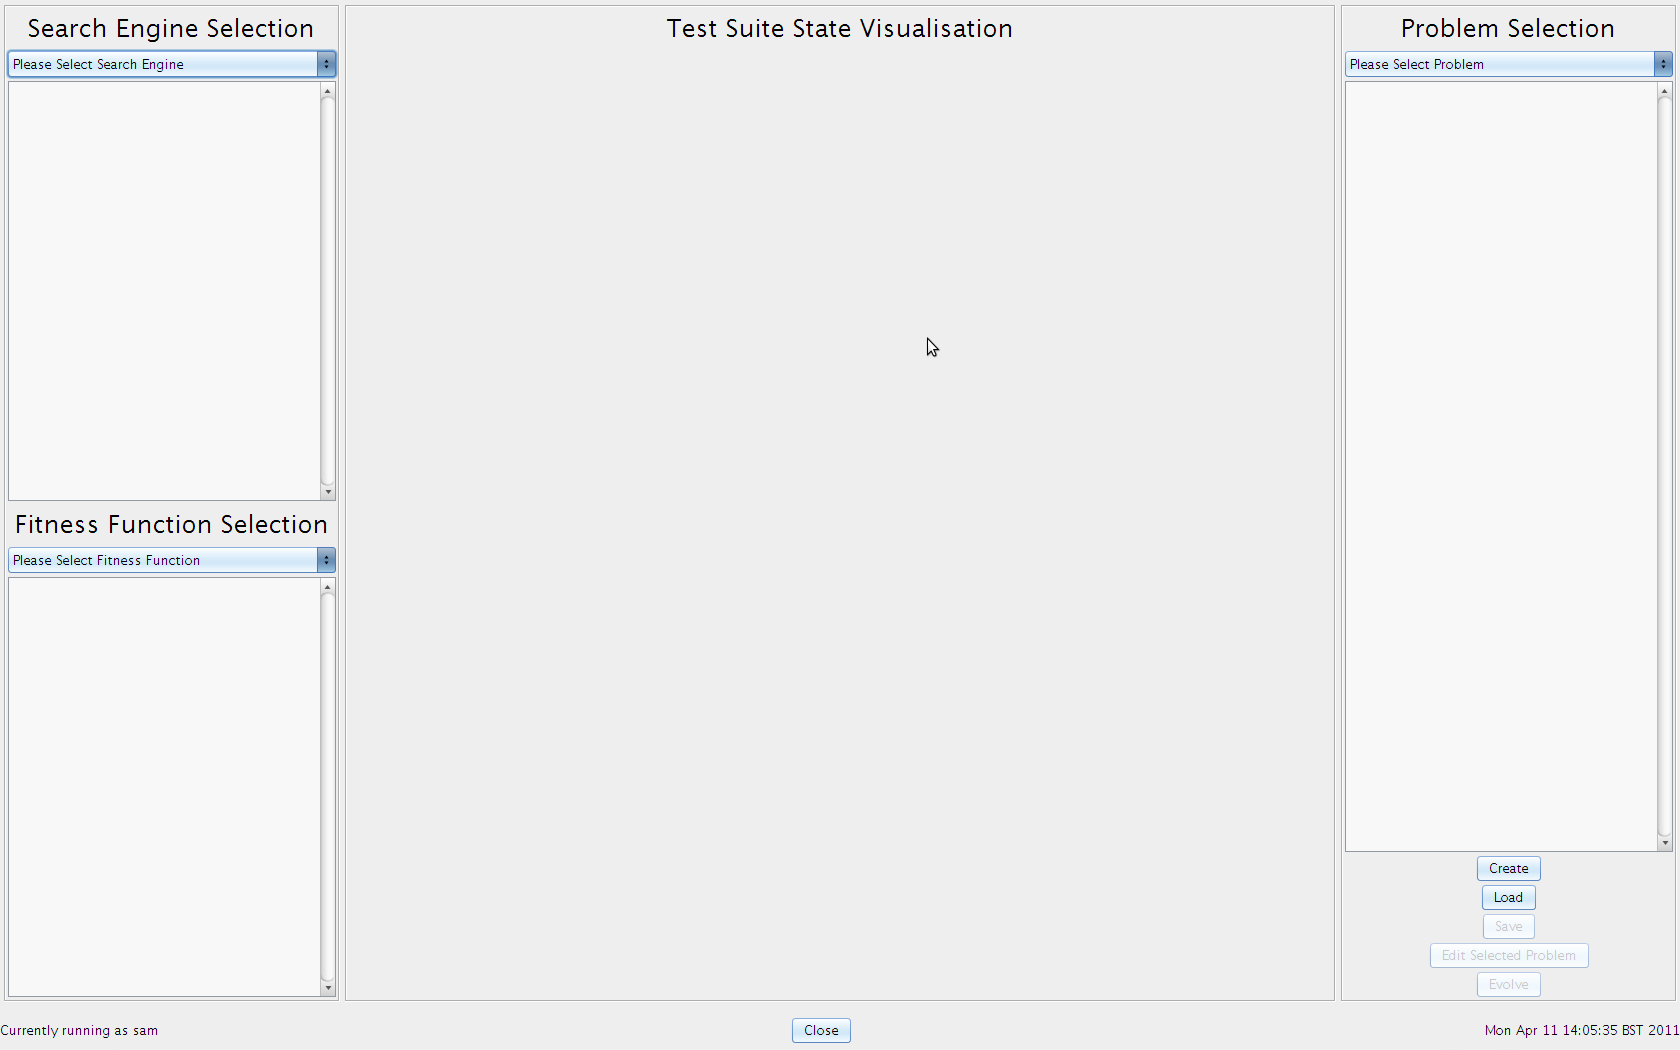
\includegraphics[width=\textwidth]{walkthrough1.png}
 \caption{Initial State of the Client GUI}
 \label{fig:walkthrough1}
\end{figure}

\begin{figure}
\begin{center}
  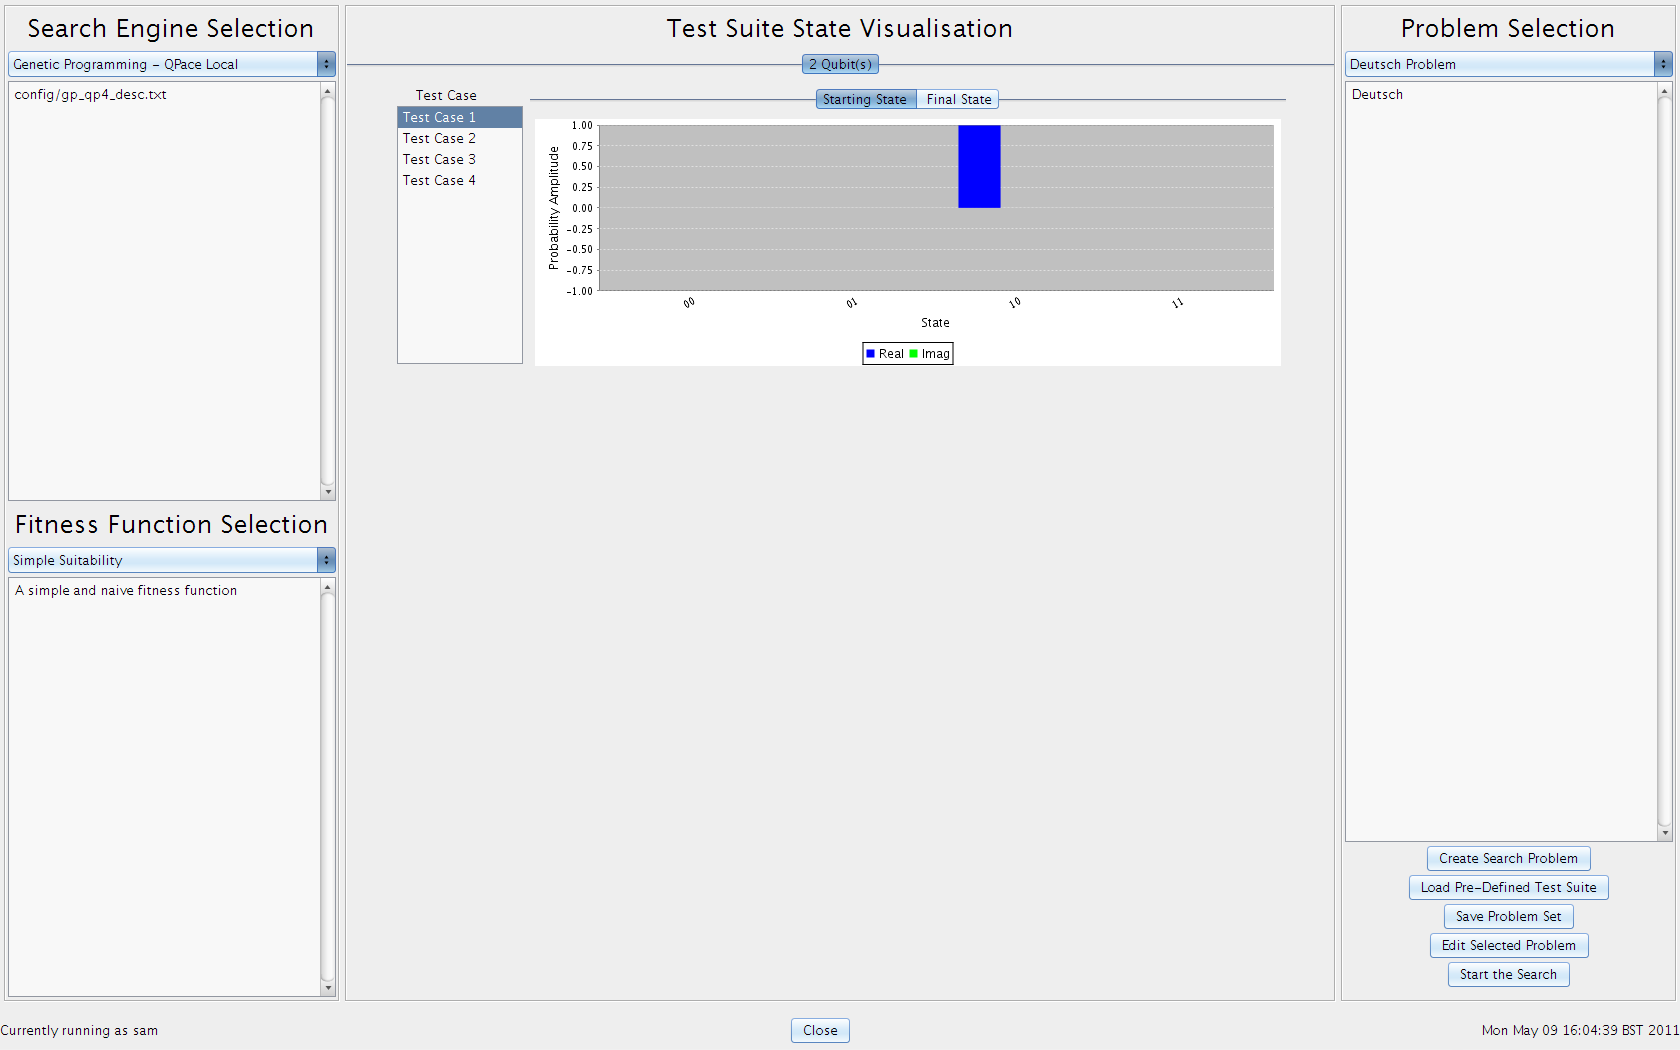
\includegraphics[width=10cm]{walkthrough2.png}
\end{center}
 \caption{Right hand menu}
 \label{fig:walkthrough2}
\end{figure}

\begin{figure}
  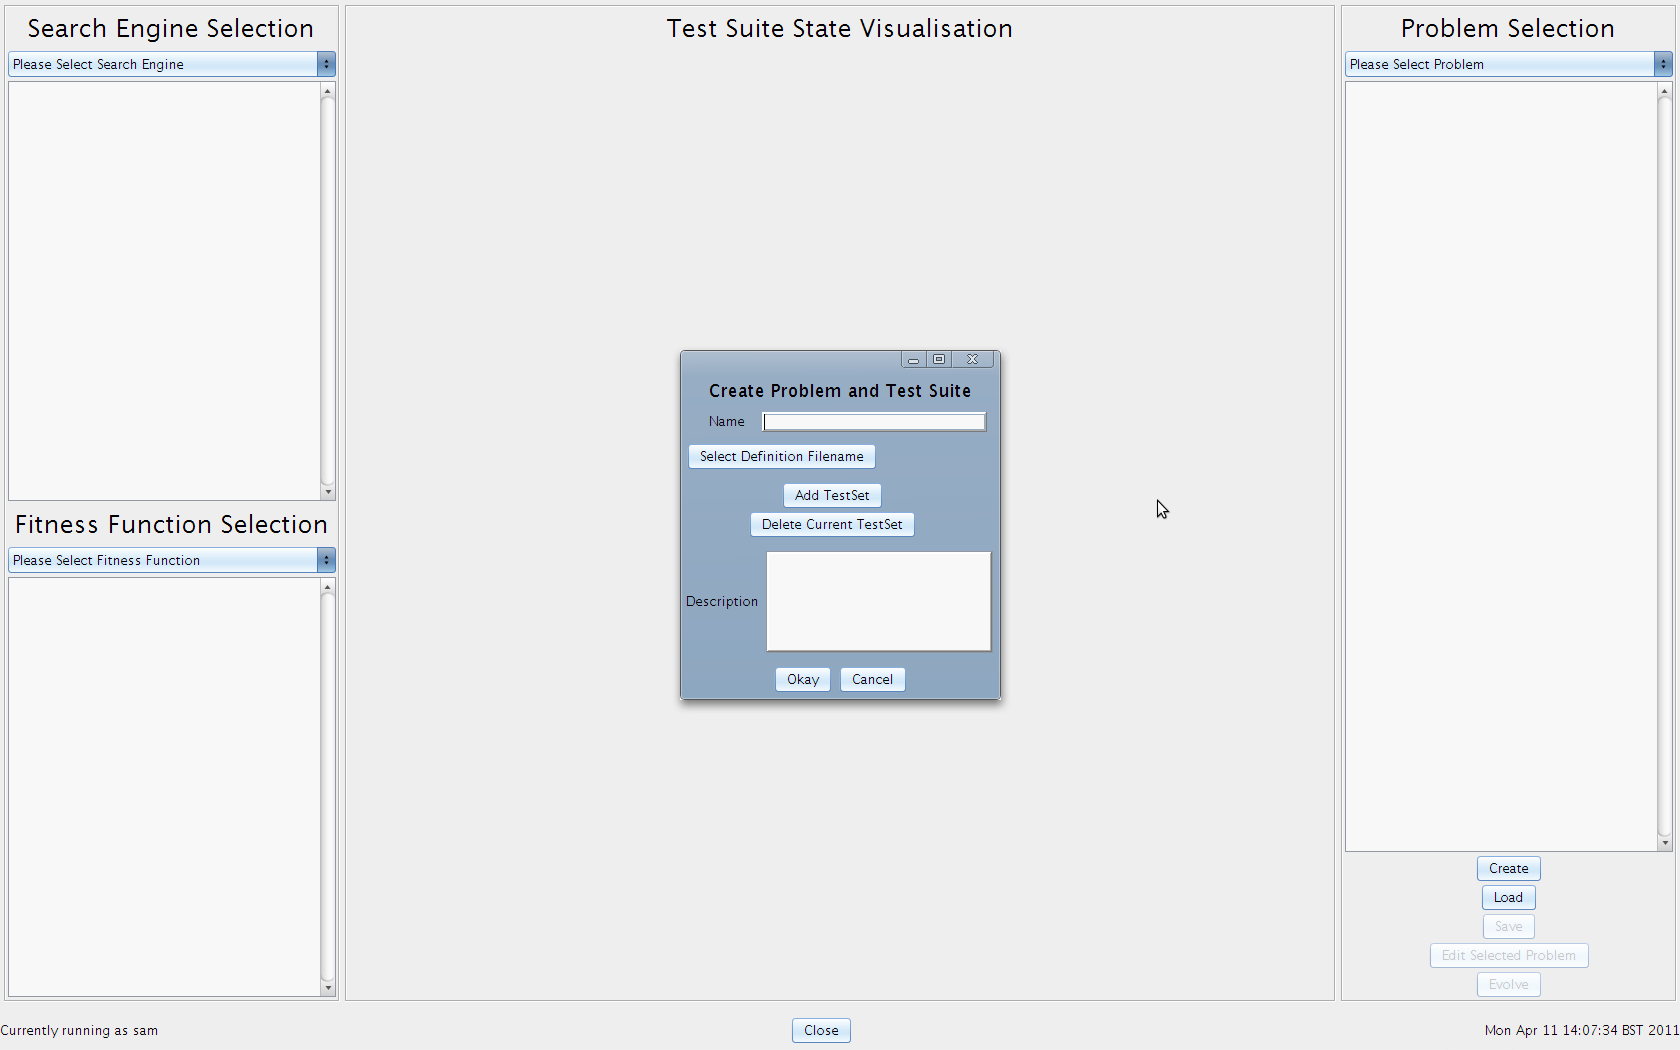
\includegraphics[width=\textwidth]{walkthrough3.png}
 \caption{Create Problem and Test Suite dialog box}
 \label{fig:walkthrough3}
\end{figure}

\begin{figure}
  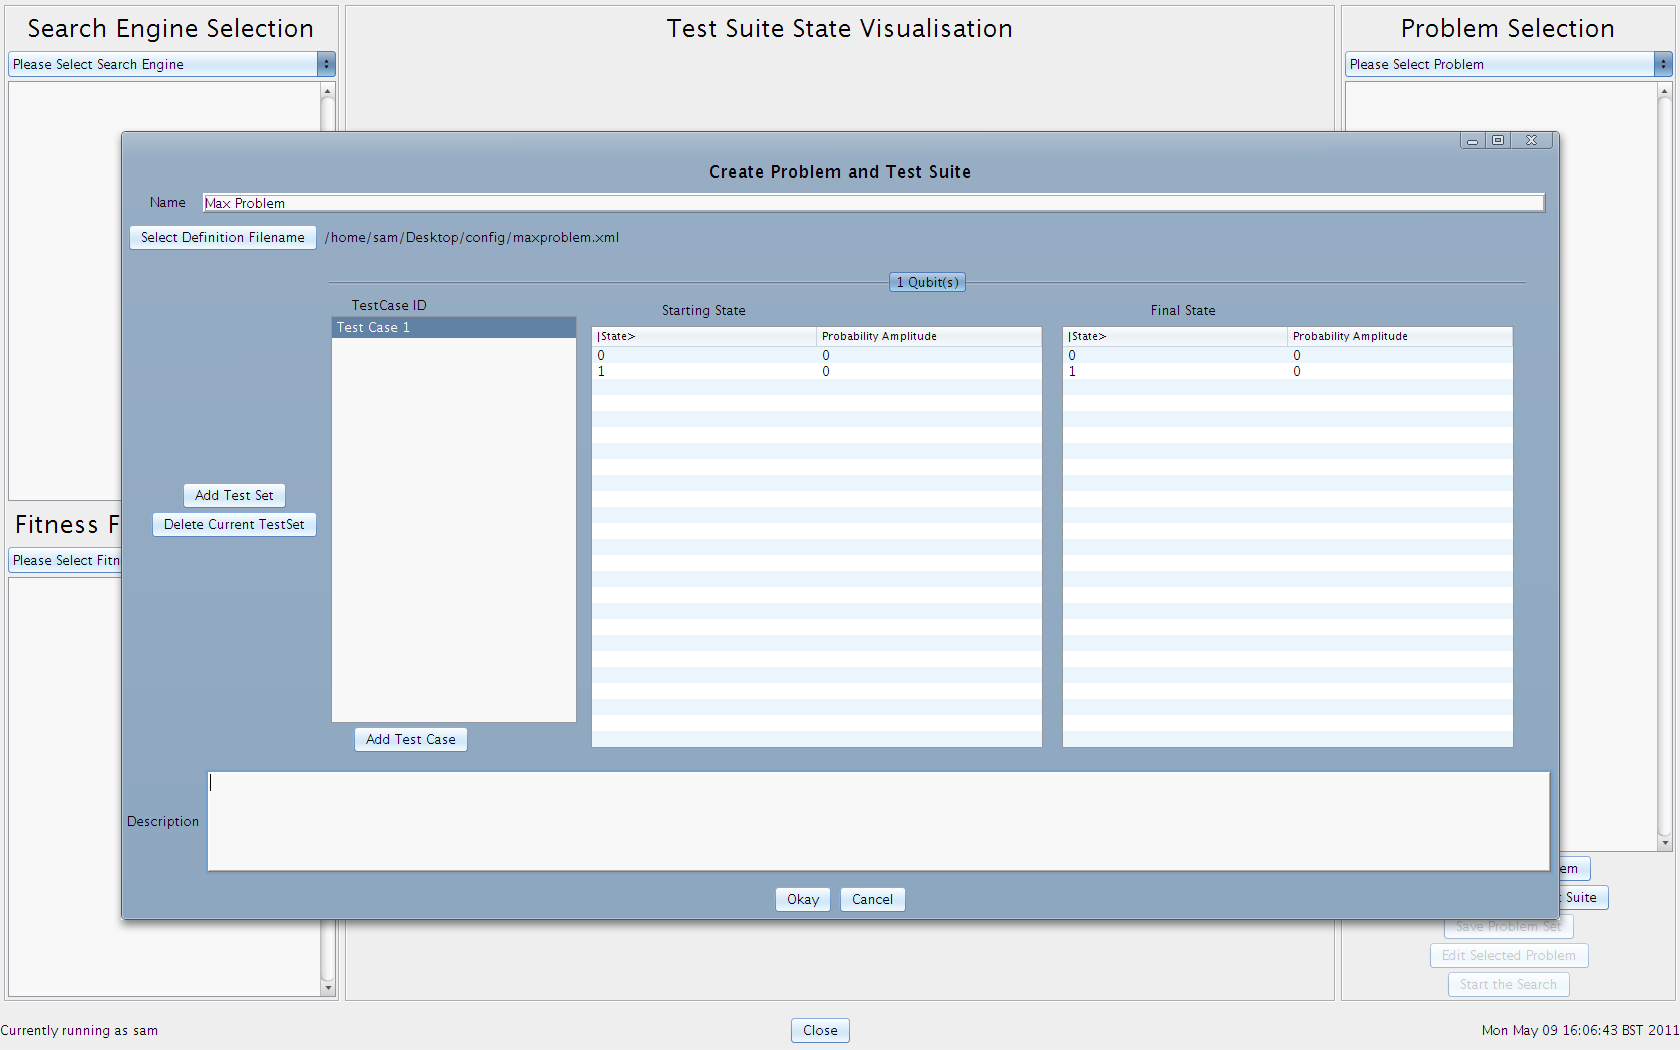
\includegraphics[width=\textwidth]{walkthrough4.png}
 \caption{Full Create Problem and Test Suite dialog box}
 \label{fig:walkthrough4}
\end{figure}

\begin{figure}
  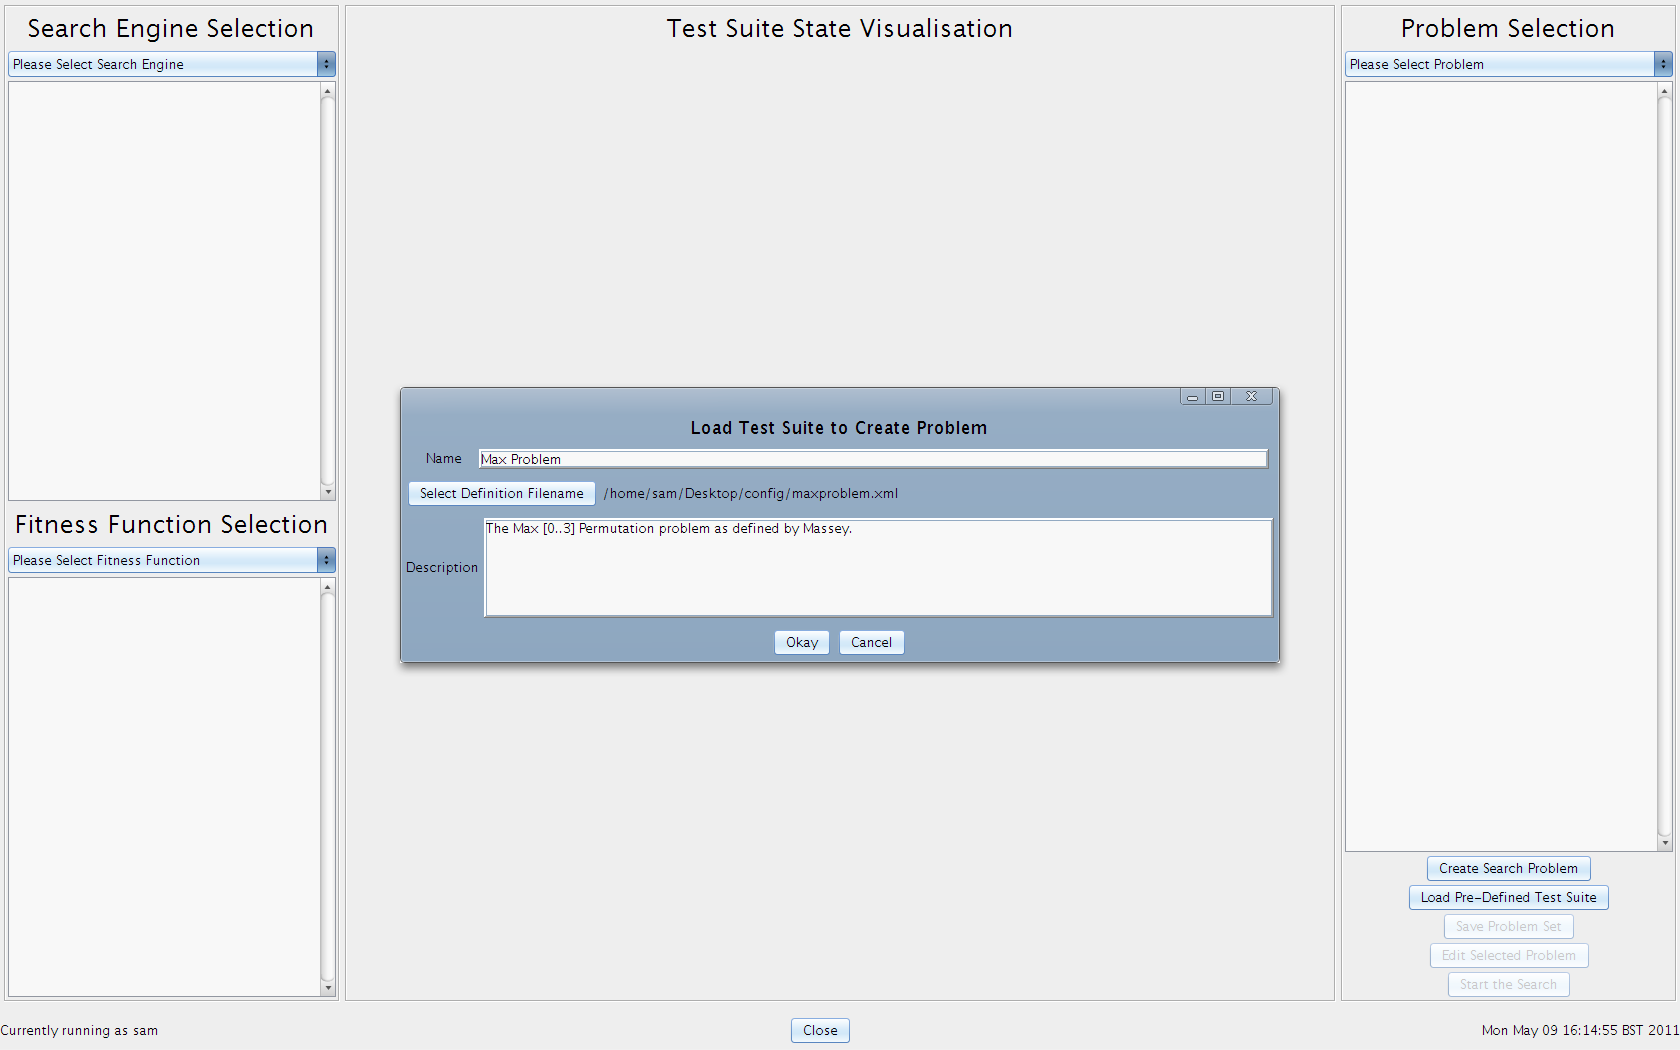
\includegraphics[width=\textwidth]{walkthrough5.png}
 \caption{Load Test Suite to Create Problem dialog box}
 \label{fig:walkthrough5}
\end{figure}

\begin{figure}
  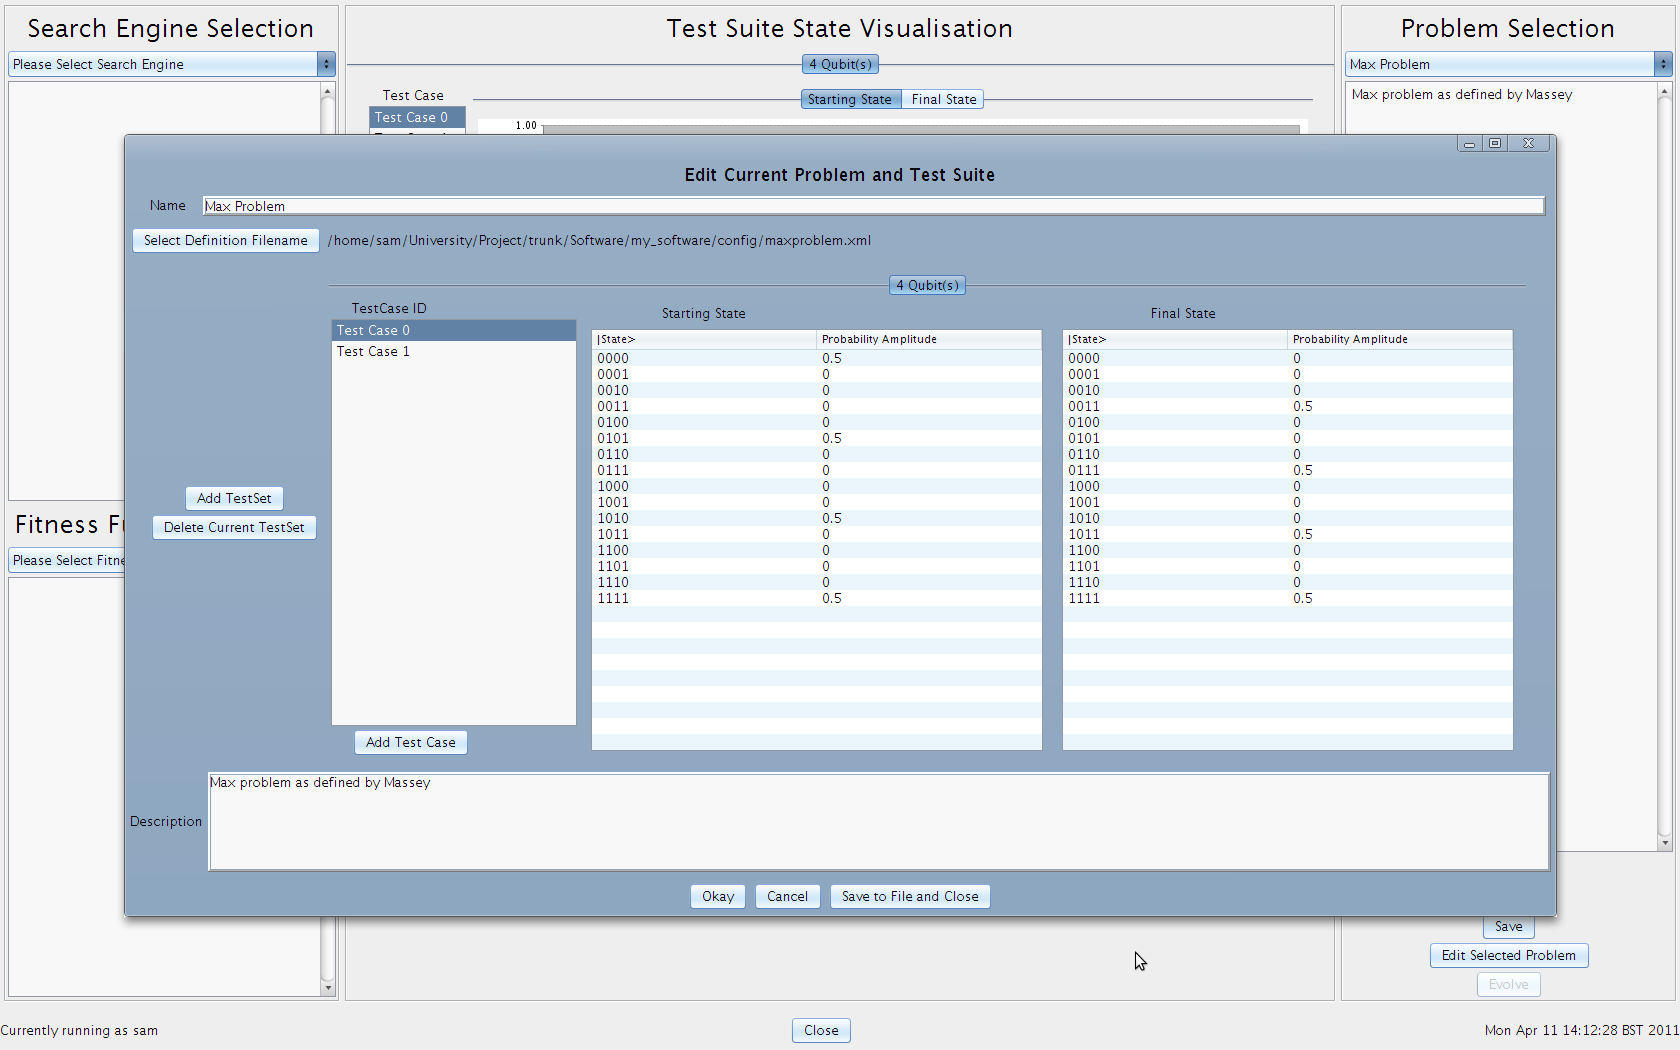
\includegraphics[width=\textwidth]{walkthrough6.png}
 \caption{Edit Current Problem and Test Suite dialog box}
 \label{fig:walkthrough6}
\end{figure}

\begin{figure}
  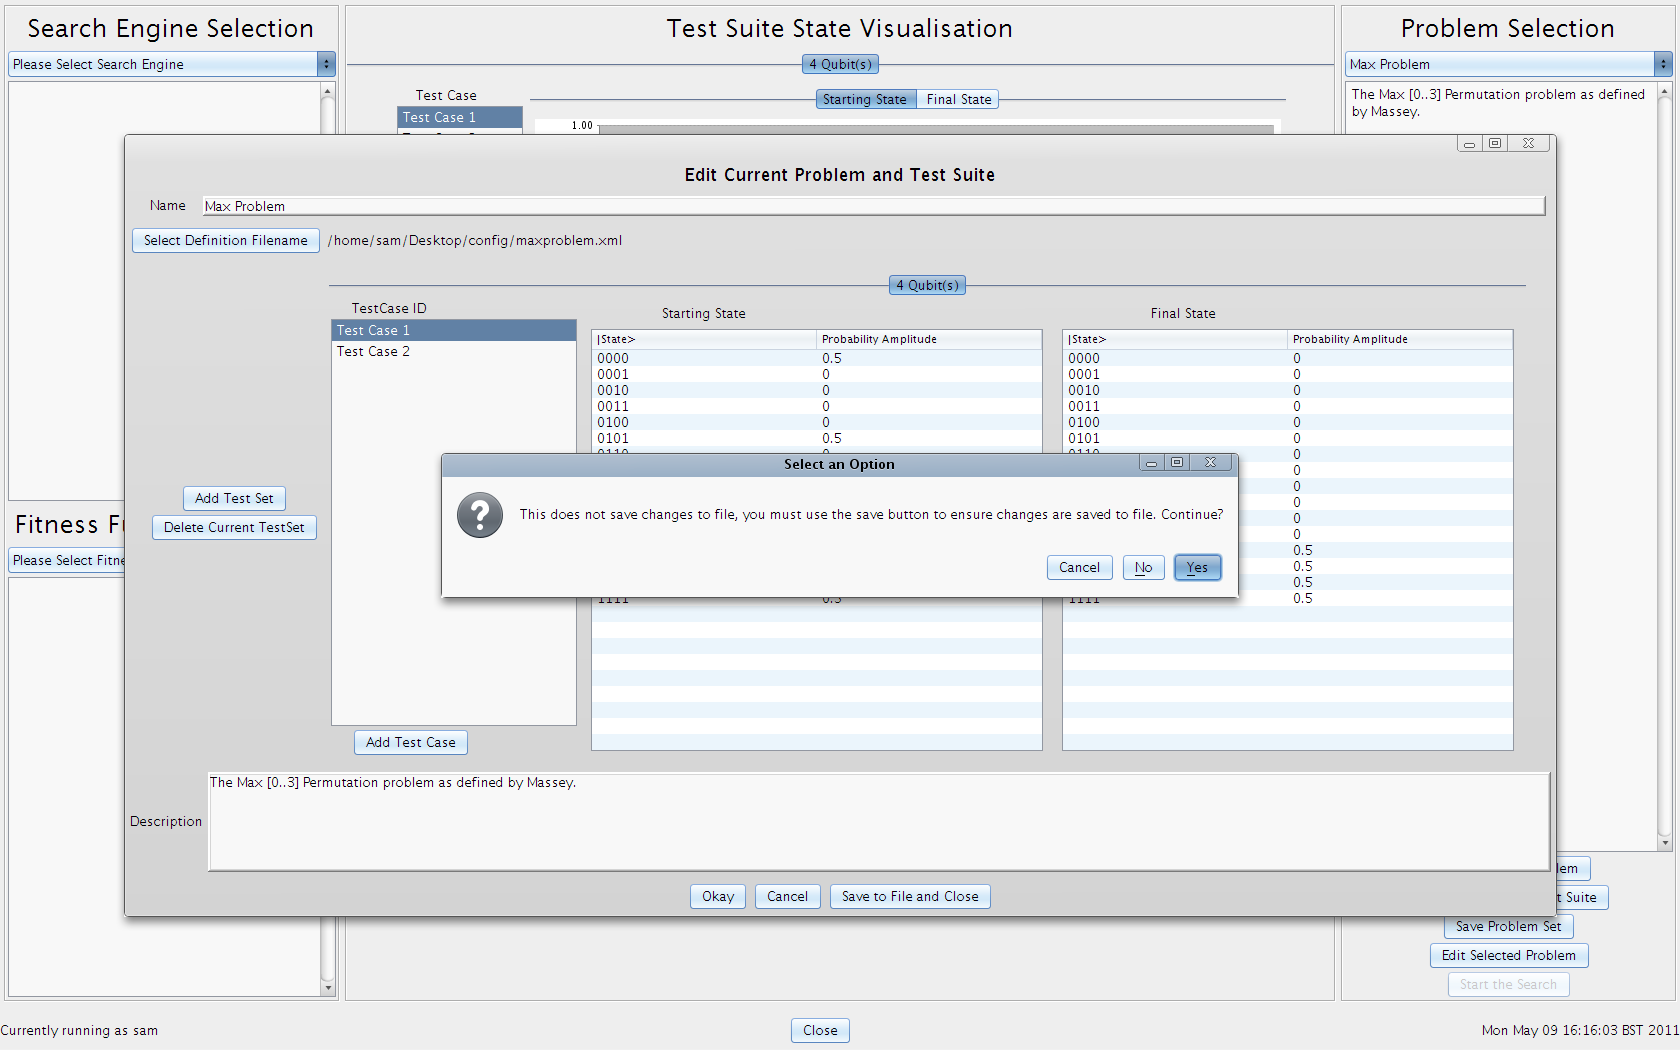
\includegraphics[width=\textwidth]{walkthrough7.png}
 \caption{Warning Produced by Pressing Okay}
 \label{fig:walkthrough7}
\end{figure}

\begin{figure}
  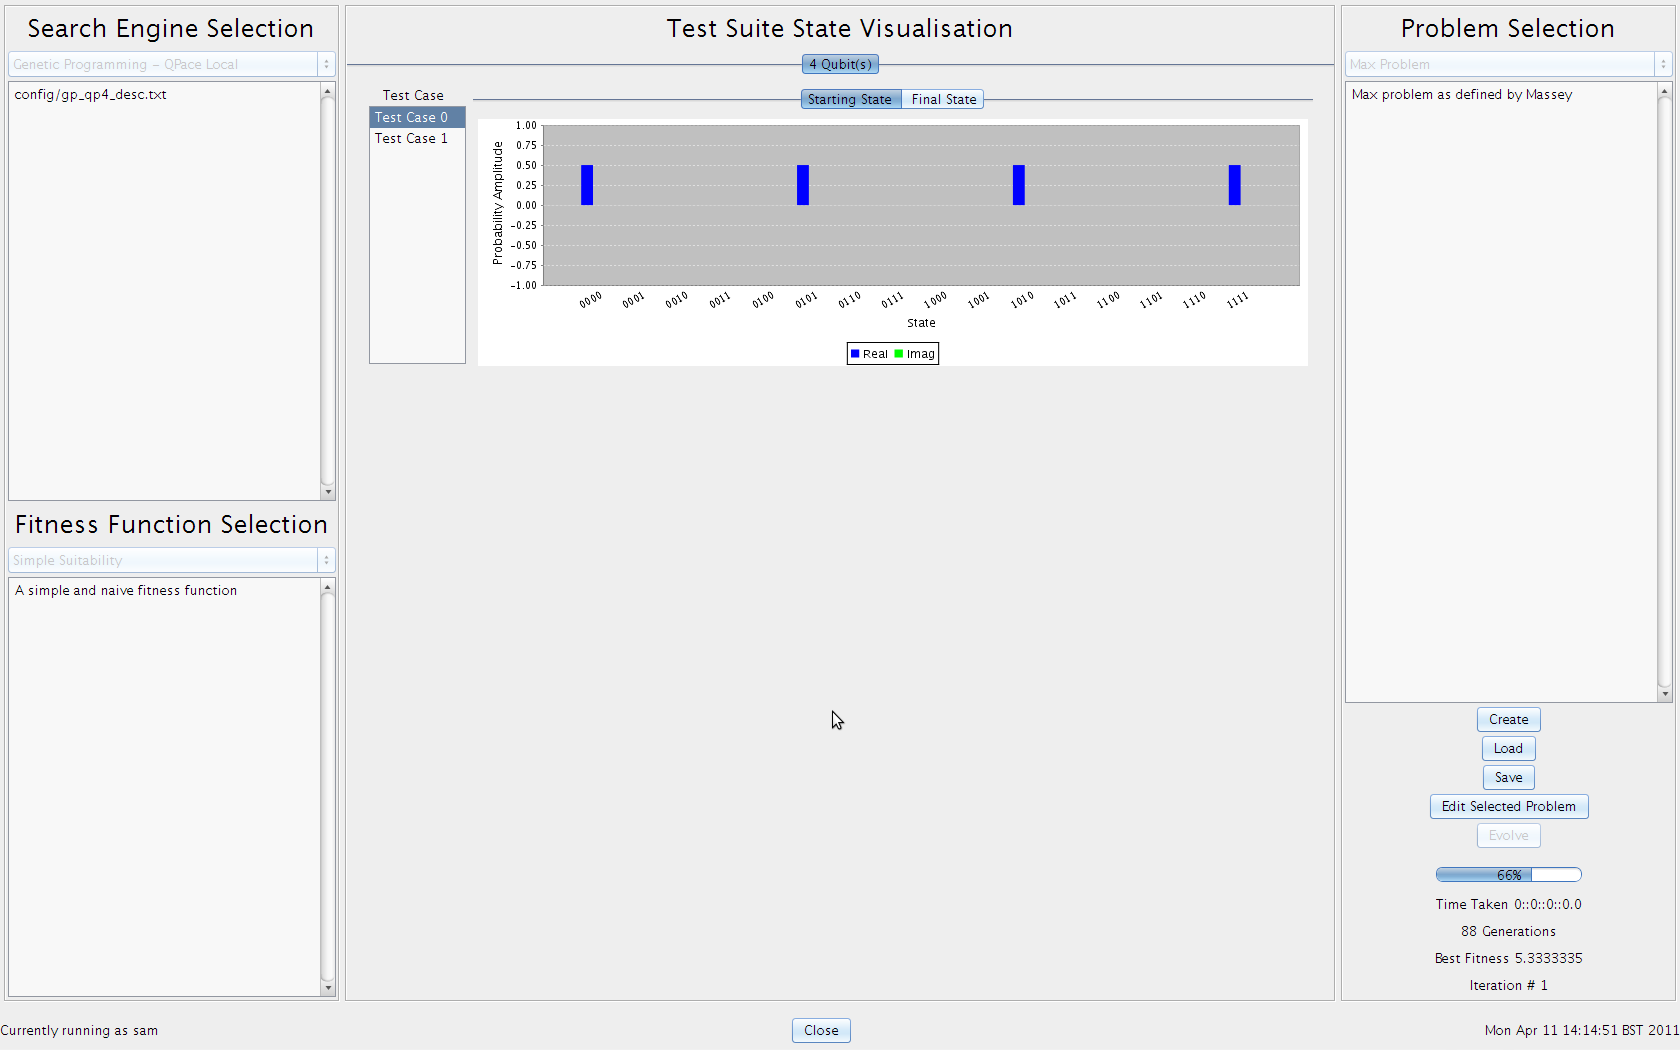
\includegraphics[width=\textwidth]{walkthrough8.png}
 \caption{Search Progress Statistics}
 \label{fig:walkthrough8}
\end{figure}

\begin{figure}
  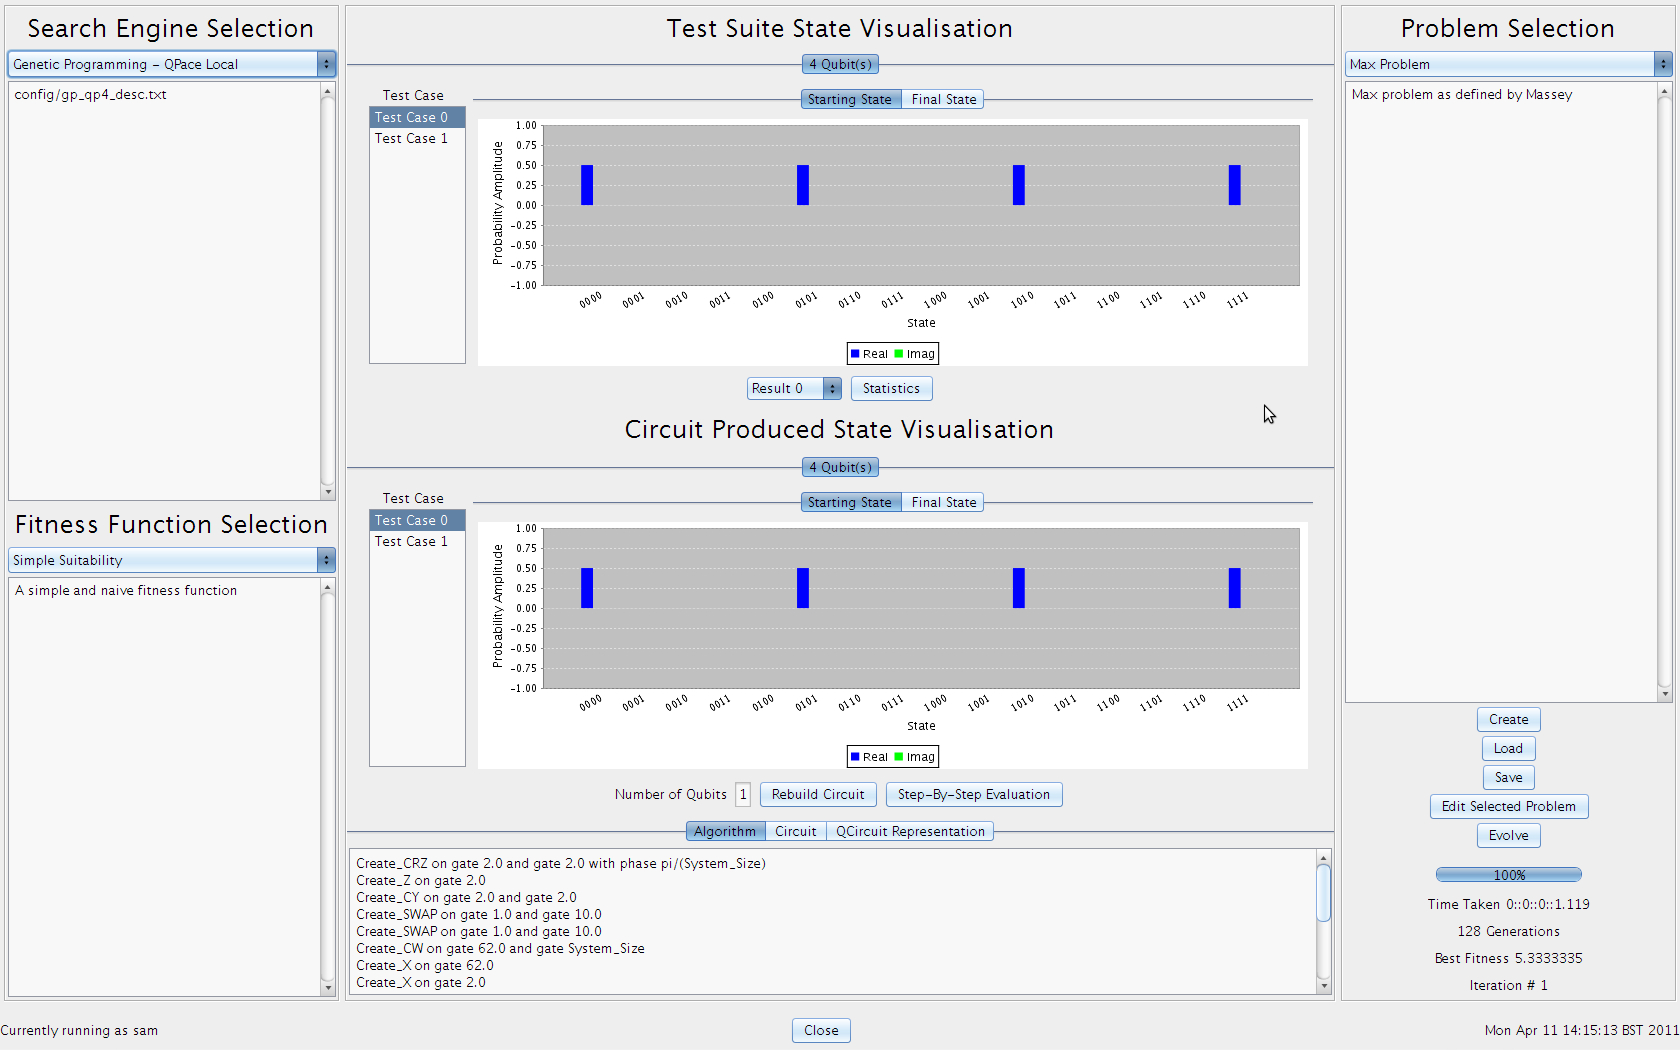
\includegraphics[width=\textwidth]{walkthrough9.png}
 \caption{Client GUI after Search is Complete}
 \label{fig:walkthrough9}
\end{figure}

\chapter{Experiment Data}

\section{Deutsch Experiment}
\label{sec:DeutschExpApp}
\subsection{Full Algorithm}
\label{sec:DeutschExpAppFullAlg}

\begin{algorithm}
 \begin{algorithmic}
\STATE Create\_Custom1 on gate Loop\_Vars[54.0]
\STATE Create\_H on gate Loop\_Vars[5.0]
\STATE Create\_CCustom1 on gate 1.0 and gate System\_Size
\STATE Create\_H on gate 1.0
\STATE Create\_V on gate 54.0
\STATE Create\_CCustom1 on gate 1.0 and gate System\_Size
\STATE Create\_H on gate 1.0
\STATE Create\_CX on gate 54.0 and gate 1.0
 \end{algorithmic}
\caption{Evolved Solution for Deutsch Problem}
\label{alg:evodeutsch}
\end{algorithm}








\clearpage
\section{Deutsch Jozsa Experiment}
\label{sec:deutschjozsa}

\begin{figure}[h!]
\centering
\subfigure[$f_1$]{
$
\begin{pmatrix}
1 & 0 & 0 & 0 & 0 & 0 & 0 & 0 \\
0 & 1 & 0 & 0 & 0 & 0 & 0 & 0\\
0 & 0 & 1 & 0 & 0 & 0 & 0 & 0\\
0 & 0 & 0 & 1 & 0 & 0 & 0 & 0\\
0 & 0 & 0 & 0 & 1 & 0 & 0 & 0\\
0 & 0 & 0 & 0 & 0 & 1 & 0 & 0\\
0 & 0 & 0 & 0 & 0 & 0 & 1 & 0\\
0 & 0 & 0 & 0 & 0 & 0 & 0 & 1
\end{pmatrix}
$
}
\subfigure[$f_2$]{
$
\begin{pmatrix}
0 & 0 & 0 & 0 & 1 & 0 & 0 & 0 \\
0 & 0 & 0 & 0 & 0 & 1 & 0 & 0\\
0 & 0 & 0 & 0 & 0 & 0 & 1 & 0\\
0 & 0 & 0 & 0 & 0 & 0 & 0 & 1\\
1 & 0 & 0 & 0 & 0 & 0 & 0 & 0\\
0 & 1 & 0 & 0 & 0 & 0 & 0 & 0\\
0 & 0 & 1 & 0 & 0 & 0 & 0 & 0\\
0 & 0 & 0 & 1 & 0 & 0 & 0 & 0
\end{pmatrix}
$
}
\subfigure[$f_3$]{
$
\begin{pmatrix}
1 & 0 & 0 & 0 & 0 & 0 & 0 & 0 \\
0 & 1 & 0 & 0 & 0 & 0 & 0 & 0\\
0 & 0 & 0 & 0 & 0 & 0 & 1 & 0\\
0 & 0 & 0 & 0 & 0 & 0 & 0 & 1\\
0 & 0 & 0 & 0 & 1 & 0 & 0 & 0\\
0 & 0 & 0 & 0 & 0 & 1 & 0 & 0\\
0 & 0 & 1 & 0 & 0 & 0 & 0 & 0\\
0 & 0 & 0 & 1 & 0 & 0 & 0 & 0
\end{pmatrix}
$
}
\\
\subfigure[$f_4$]{
$
\begin{pmatrix}
1 & 0 & 0 & 0 & 0 & 0 & 0 & 0 \\
0 & 0 & 0 & 0 & 0 & 1 & 0 & 0\\
0 & 0 & 1 & 0 & 0 & 0 & 0 & 0\\
0 & 0 & 0 & 0 & 0 & 0 & 0 & 1\\
0 & 0 & 0 & 0 & 1 & 0 & 0 & 0\\
0 & 1 & 0 & 0 & 0 & 0 & 0 & 0\\
0 & 0 & 0 & 0 & 0 & 0 & 1 & 0\\
0 & 0 & 0 & 1 & 0 & 0 & 0 & 0
\end{pmatrix}
$
}
\subfigure[$f_5$]{
$
\begin{pmatrix}
0 & 0 & 0 & 0 & 1 & 0 & 0 & 0 \\
0 & 1 & 0 & 0 & 0 & 0 & 0 & 0\\
0 & 0 & 1 & 0 & 0 & 0 & 0 & 0\\
0 & 0 & 0 & 0 & 0 & 0 & 0 & 1\\
1 & 0 & 0 & 0 & 0 & 0 & 0 & 0\\
0 & 0 & 0 & 0 & 0 & 1 & 0 & 0\\
0 & 0 & 0 & 0 & 0 & 0 & 1 & 0\\
0 & 0 & 0 & 1 & 0 & 0 & 0 & 0
\end{pmatrix}
$
}
\subfigure[$f_6$]{
$
\begin{pmatrix}
1 & 0 & 0 & 0 & 0 & 0 & 0 & 0 \\
0 & 0 & 0 & 0 & 0 & 1 & 0 & 0\\
0 & 0 & 0 & 0 & 0 & 0 & 1 & 0\\
0 & 0 & 0 & 1 & 0 & 0 & 0 & 0\\
0 & 0 & 0 & 0 & 1 & 0 & 0 & 0\\
0 & 1 & 0 & 0 & 0 & 0 & 0 & 0\\
0 & 0 & 1 & 0 & 0 & 0 & 0 & 0\\
0 & 0 & 0 & 0 & 0 & 0 & 0 & 1
\end{pmatrix}
$
}
\\
\subfigure[$f_7$]{
$
\begin{pmatrix}
0 & 0 & 0 & 0 & 1 & 0 & 0 & 0 \\
0 & 1 & 0 & 0 & 0 & 0 & 0 & 0\\
0 & 0 & 0 & 0 & 0 & 0 & 1 & 0\\
0 & 0 & 0 & 1 & 0 & 0 & 0 & 0\\
1 & 0 & 0 & 0 & 0 & 0 & 0 & 0\\
0 & 0 & 0 & 0 & 0 & 1 & 0 & 0\\
0 & 0 & 1 & 0 & 0 & 0 & 0 & 0\\
0 & 0 & 0 & 0 & 0 & 0 & 0 & 1
\end{pmatrix}
$
}
\subfigure[$f_8$]{
$
\begin{pmatrix}
0 & 0 & 0 & 0 & 1 & 0 & 0 & 0 \\
0 & 0 & 0 & 0 & 0 & 1 & 0 & 0\\
0 & 0 & 1 & 0 & 0 & 0 & 0 & 0\\
0 & 0 & 0 & 1 & 0 & 0 & 0 & 0\\
1 & 0 & 0 & 0 & 0 & 0 & 0 & 0\\
0 & 1 & 0 & 0 & 0 & 0 & 0 & 0\\
0 & 0 & 0 & 0 & 0 & 0 & 1 & 0\\
0 & 0 & 0 & 0 & 0 & 0 & 0 & 1
\end{pmatrix}
$
}
\caption{Matricies of Custom Gates Implementing the Eight Possible Functions}
 \label{fig:deutschjozsafunctions}
\end{figure}

\clearpage
\subsection{Search Parameters}
\label{sec:deutschjozsasearchparams}

\begin{figure}[h!]
\begin{center}
 \begin{tabular}{|cc|cc|}
\hline
  Population Size & 128 & Generations & 300 \\
  \# of Breeder Threads & 8 & \# of Evaluation Threads & 8 \\
  \# of Elites & 1 & Number of Iterations & 1 \\
  Minimum Initial Tree Depth & 10 & Maximum Initial Tree Depth & 20 \\
  CrossOver Rate & 0.9 & Mutation Rate & 0.0033846154 \\
\hline
 \end{tabular}
 \begin{tabular}{cc}
  \textbf{Search Engine} & Genetic Programming - QPace Local \\
  \textbf{Suitability Measure} & Simple Suitability - Non-Zero Count \\
 \end{tabular}
\begin{tabular}{|ccccccc|}
\hline
  Create\_H & Create\_X& Create\_Y& Create\_Z & Create\_R & Create\_Custom1 & Body \\
  Create\_CH & Create\_CX & Create\_CY & Create\_CZ & Create\_CR & Create\_CCustom1 & Iterate \\
   & Create\_CCX &  & &  &  &  \\
\hline
 \end{tabular}
\end{center}
\caption{Search Parameters used for Deutsch Jozsa Search}
\label{fig:deutschjozsaparams}
\end{figure}

\subsection{Full Algorithm}
\label{sec:DeutschJozsaExpAppFullAlg}

\begin{algorithm}
 \begin{algorithmic}
\STATE Create\_CR on gate 2.0 and gate 6.0 with phase 1.0
\STATE Create\_H on gate 2.0
\STATE Create\_H on gate 3.0
\STATE Create\_H on gate 1.0
\STATE Create\_Custom1 on gate 1.0
\STATE Create\_CR on gate Loop\_Vars[3.0] and gate 48.0 with phase Loop\_Vars[2.0]
\STATE Create\_CR on gate 2.0 and gate 6.0 with phase 1.0
\STATE Create\_H on gate 39.0
\STATE Create\_CR on gate 2.0 and gate 6.0 with phase 1.0
\STATE Create\_H on gate 2.0
\STATE Create\_H on gate 3.0
\STATE Create\_H on gate 31.0
\STATE Create\_CR on gate 2.0 and gate 6.0 with phase 1.0
\STATE Create\_H on gate Loop\_Vars[2.0]
\STATE Create\_H on gate 1.0
\STATE Create\_CR on gate 79.0 and gate Loop\_Vars[10.0] with phase Loop\_Vars[2.0]
 \end{algorithmic}
\caption{Evolved Solution for Deutsch Jozsa Problem}
\label{alg:evodeutschjozsa}
\end{algorithm}

\clearpage
\subsection{Full Circuits}
\label{sec:DeutschJozsaExpAppFullCirs}
\begin{figure}[h!]
\[
\Qcircuit @C=1.0em @R=.7em {
&\gate{H}&\qw&\qw&\qw&\\%2
&\qw&\gate{H}&\gate{C0}&\gate{H}&\\%1
}
\]
\caption{Deutsch Jozsa Solution - Two Qubits }
\end{figure}
\begin{figure}[h!]
\[
\Qcircuit @C=1.0em @R=.7em {
&\qw&\gate{H}&\qw&\qw&\qw&\qw&\\%3
&\gate{H}&\qw&\qw&\qw&\gate{H}&\qw&\\%2
&\qw&\qw&\gate{H}&\gate{C0}&\qw&\gate{H}&\\%1
}
\]
\caption{Deutsch Jozsa Solution - Three Qubits }
\end{figure}
\begin{figure}[h!]
\[
\Qcircuit @C=1.0em @R=.7em {
&\qw&\qw&\qw&\qw&\qw&\qw&\gate{H}&\qw&\\%4
&\qw&\gate{H}&\qw&\qw&\qw&\gate{H}&\qw&\qw&\\%3
&\gate{H}&\qw&\qw&\qw&\gate{H}&\qw&\qw&\qw&\\%2
&\qw&\qw&\gate{H}&\gate{C0}&\qw&\qw&\qw&\gate{H}&\\%1
}
\]
\caption{Deutsch Jozsa Solution - Four Qubits }
\label{fig:evodeutschjozsafourq}
\end{figure}

\clearpage
\section{0..3 Max Permutation Problem}
\label{sec:maxpermsol}

\subsection{Search Parameters}
\label{sec:maxpermsearchparams}

\begin{figure}[h!]
\begin{center}
 \begin{tabular}{|cc|cc|}
\hline
  Population Size & 128 & Generations & 128 \\
  \# of Breeder Threads & 8 & \# of Evaluation Threads & 8 \\
  \# of Elites & 1 & Number of Iterations & 1 \\
  Minimum Initial Tree Depth & 1 & Maximum Initial Tree Depth & 30 \\
  CrossOver Rate & 0.9 & Mutation Rate & 0.003846154 \\
\hline
 \end{tabular}
 \begin{tabular}{cc}
  \textbf{Search Engine} & Genetic Programming - QPace Local \\
  \textbf{Suitability Measure} & Simple Suitability - Zero Focessed \\
 \end{tabular}
 \begin{tabular}{|ccccc|}
\hline
  Create\_H & Create\_X & Create\_R & Body & Iterate \\
  Create\_CH & Create\_CX & Create\_CR & Create\_CCX & RevIterate \\
\hline
 \end{tabular}
\end{center}
\caption{Search Parameters Used for 0..3 Max Permutation Problem}
\label{fig:maxpermparams}
\end{figure}

\clearpage
\subsection{Algorithm}
\begin{algorithm}
 \begin{algorithmic}
\STATE \{
\STATE Iterate for 10.0 iterations \{
\STATE \}
\STATE \}
\STATE Create\_X on gate Loop\_Vars[8.0]
\STATE Create\_CX on gate 17.0 and gate 45.0
\STATE Create\_CH on gate 7.0 and gate 17.0
\STATE Iterate for 95.0 iterations \{
\STATE Create\_R on gate Loop\_Vars[4.0] with phase Loop\_Vars[1.0]
\STATE \}
\STATE Create\_H on gate 102.0
\STATE \{
\STATE \{
\STATE Create\_CCX on gate 2.0 and gate 1.0 with phase 2.0
\STATE \}
\STATE Create\_X on gate 2.0
\STATE \}
\STATE Iterate for 10.0 iterations \{
\STATE \}
\STATE Create\_CCX on gate System\_Size and gate 1.0 with phase 2.0
\end{algorithmic}
\caption{Full Algorithm to Produce the Solution for the Max Permutation Problem}
\label{alg:03permfullalg}
\end{algorithm}

\clearpage
\subsection{Measurement Probabilities}
\label{sec:maxpermmeasprobs}
\centering
 \begin{tabular}{c|c|c|c|c|}
\textbf{Test Case} & $\ket{00}$& $\ket{01}$& $\ket{10}$& $\ket{11}$ \\
1 & 0.25 & 0.00 & 0.25 & \textbf{0.50} \\
2 & 0.00 & 0.25 & \textbf{0.50} & 0.25 \\
3 & 0.25 & 0.00 & 0.25 & \textbf{0.50} \\
4 & 0.00 & 0.25 & \textbf{0.50} & 0.25 \\
5 & 0.25 & \textbf{0.50} & 0.25 & 0.00 \\
6 & 0.25 & \textbf{0.50} & 0.25 & 0.00 \\
7 & 0.25 & 0.00 & 0.25 & \textbf{0.50} \\
8 & 0.00 & 0.25 & \textbf{0.50} & 0.25 \\
9 & 0.25 & 0.00 & 0.25 & \textbf{0.50} \\
10 & 0.00 & 0.25 & \textbf{0.50} & 0.25 \\
11 & 0.25 & \textbf{0.50} & 0.25 & 0.00 \\
12 & 0.25 & \textbf{0.50} & 0.25 & 0.00 \\
13 & 0.25 & 0.00 & 0.25 & \textbf{0.50} \\
14 & 0.00 & 0.25 & \textbf{0.50} & 0.25 \\
15 & 0.25 & 0.00 & 0.25 & \textbf{0.50} \\
16 & 0.00 & 0.25 & \textbf{0.50} & 0.25 \\
17 & 0.25 & \textbf{0.50} & 0.25 & 0.00 \\
18 & 0.25 & \textbf{0.50} & 0.25 & 0.00 \\
19 & \textbf{0.50} & 0.25 & 0.00 & 0.25 \\
20 & \textbf{0.50} & 0.25 & 0.00 & 0.25 \\
21 & \textbf{0.50} & 0.25 & 0.00 & 0.25 \\
22 & \textbf{0.50} & 0.25 & 0.00 & 0.25 \\
23 & \textbf{0.50} & 0.25 & 0.00 & 0.25 \\
24 & \textbf{0.50} & 0.25 & 0.00 & 0.25
 \end{tabular}

The bold values are the probability of the desired states, the solution states.

\clearpage
\section{Quantum Fourier Transform Experiment}
\label{sec:quantfourtransexp}


\begin{figure}[h!]
\centering
\subfigure[Test Case $1$]{
$
\begin{pmatrix}
1 \\
0 \\
0 \\
0  
\end{pmatrix}
\rightarrow
\begin{pmatrix}
   0.50000 \\
   0.50000 \\
   0.50000 \\
   0.50000
\end{pmatrix}
$

}
\subfigure[Test Case $2$]{
$
\begin{pmatrix}
0 \\
1 \\
0 \\
0  
\end{pmatrix}
\rightarrow
\begin{pmatrix}
   0.50000 + 0.00000i \\
   0.00000 + 0.50000i \\
  -0.50000 + 0.00000i \\
  -0.00000 - 0.50000i  
\end{pmatrix}
$
}
\subfigure[Test Case $3$]{
$
\begin{pmatrix}
0 \\
0 \\
1 \\
0  
\end{pmatrix}
\rightarrow
\begin{pmatrix}
   0.50000 + 0.00000i \\
  -0.50000 + 0.00000i \\
   0.50000 - 0.00000i \\
  -0.50000 + 0.00000i 
\end{pmatrix}
$
}
\subfigure[Test Case $4$]{
$
\begin{pmatrix}
0 \\
0 \\
0 \\
1 
\end{pmatrix}
\rightarrow
\begin{pmatrix}
   0.50000 + 0.00000i \\
  -0.00000 - 0.50000i \\
  -0.50000 + 0.00000i \\
   0.00000 + 0.50000i 
\end{pmatrix}
$
}
\caption{Test Cases for Two Qubits}
 \label{fig:qfttwoqubits}
\end{figure}


\begin{figure}[h!]
\centering
\subfigure[Test Case $1$]{
$
\begin{pmatrix}
1 \\
0 \\
0 \\
0 \\
0 \\
0 \\
0 \\
0  
\end{pmatrix}
\rightarrow
\begin{pmatrix}
0.35355 + 0.00000i \\
0.35355 + 0.00000i \\
0.35355 + 0.00000i \\
0.35355 + 0.00000i \\
0.35355 + 0.00000i \\
0.35355 + 0.00000i \\
0.35355 + 0.00000i \\
0.35355 + 0.00000i
\end{pmatrix}
$

}
\subfigure[Test Case $2$]{
$
\begin{pmatrix}
0 \\
1 \\
0 \\
0 \\
0 \\
0 \\
0 \\
0  
\end{pmatrix}
\rightarrow
\begin{pmatrix}
0.35355 + 0.00000i \\
0.25000 + 0.25000i \\
0.00000 + 0.35355i \\
-0.25000 + 0.25000i \\
-0.35355 + 0.00000i \\
-0.25000 - 0.25000i \\
-0.00000 - 0.35355i \\
0.25000 - 0.25000i
\end{pmatrix}
$
}
\subfigure[Test Case $3$]{
$
\begin{pmatrix}
0 \\
0 \\
1 \\
0 \\
0 \\
0 \\
0 \\
0  
\end{pmatrix}
\rightarrow
\begin{pmatrix}
   0.35355 + 0.00000i \\
   0.00000 + 0.35355i \\
  -0.35355 + 0.00000i \\
  -0.00000 - 0.35355i \\
   0.35355 - 0.00000i \\
   0.00000 + 0.35355i \\
  -0.35355 + 0.00000i \\
  -0.00000 - 0.35355i
\end{pmatrix}
$
}
\subfigure[Test Case $4$]{
$
\begin{pmatrix}
0 \\
0 \\
0 \\
1 \\
0 \\
0 \\
0 \\
0
\end{pmatrix}
\rightarrow
\begin{pmatrix}
   0.35355 + 0.00000i \\
  -0.25000 + 0.25000i \\
  -0.00000 - 0.35355i \\
   0.25000 + 0.25000i \\
  -0.35355 + 0.00000i \\
   0.25000 - 0.25000i \\
   0.00000 + 0.35355i \\
  -0.25000 - 0.25000i
\end{pmatrix}
$
}
\subfigure[Test Case $5$]{
$
\begin{pmatrix}
0 \\
0 \\
0 \\
0 \\
1 \\
0 \\
0 \\
0
\end{pmatrix}
\rightarrow
\begin{pmatrix}
   0.35355 + 0.00000i \\
  -0.35355 + 0.00000i \\
   0.35355 - 0.00000i \\
  -0.35355 + 0.00000i \\
   0.35355 - 0.00000i \\
  -0.35355 + 0.00000i \\
   0.35355 - 0.00000i \\
  -0.35355 + 0.00000i
\end{pmatrix}
$
}
\subfigure[Test Case $6$]{
$
\begin{pmatrix}
0 \\
0 \\
0 \\
0 \\
0 \\
1 \\
0 \\
0
\end{pmatrix}
\rightarrow
\begin{pmatrix}
   0.35355 + 0.00000i \\
  -0.25000 - 0.25000i \\
   0.00000 + 0.35355i \\
   0.25000 - 0.25000i \\
  -0.35355 + 0.00000i \\
   0.25000 + 0.25000i \\
  -0.00000 - 0.35355i \\
  -0.25000 + 0.25000i
\end{pmatrix}
$
}
\subfigure[Test Case $7$]{
$
\begin{pmatrix}
0 \\
0 \\
0 \\
0 \\
0 \\
0 \\
1 \\
0
\end{pmatrix}
\rightarrow
\begin{pmatrix}
   0.35355 + 0.00000i \\
  -0.00000 - 0.35355i \\
  -0.35355 + 0.00000i \\
   0.00000 + 0.35355i \\
   0.35355 - 0.00000i \\
  -0.00000 - 0.35355i \\
  -0.35355 + 0.00000i \\
   0.00000 + 0.35355i
\end{pmatrix}
$
}
\subfigure[Test Case $8$]{
$
\begin{pmatrix}
0 \\
0 \\
0 \\
0 \\
0 \\
0 \\
0 \\
1
\end{pmatrix}
\rightarrow
\begin{pmatrix}
   0.35355 + 0.00000i \\
   0.25000 - 0.25000i \\
  -0.00000 - 0.35355i \\
  -0.25000 - 0.25000i \\
  -0.35355 + 0.00000i \\
  -0.25000 + 0.25000i \\
   0.00000 + 0.35355i \\
   0.25000 + 0.25000i
\end{pmatrix}
$
}
\caption{Test Cases for Two Qubits}
 \label{fig:qftthreequbits}
\end{figure}

\clearpage
\subsection{Search Parameters}
\label{sec:qftsearchparams}

\begin{figure}[h!]
\begin{center}
 \begin{tabular}{|cc|cc|}
\hline
  Population Size & 1280 & Generations & 1280 \\
  \# of Breeder Threads & 8 & \# of Evaluation Threads & 8 \\
  \# of Elites & 1 & Number of Iterations & 1 \\
  Minimum Initial Tree Depth & 10 & Maximum Initial Tree Depth & 20 \\
  CrossOver Rate & 0.9 & Mutation Rate & 0.003846154 \\
\hline
 \end{tabular}
 \begin{tabular}{cc}
  \textbf{Search Engine} & Genetic Programming - QPace Local \\
  \textbf{Suitability Measure} & Phase Sensitive \\
 \end{tabular}
 \begin{tabular}{|cccc|}
\hline
  Create\_H & Create\_R & Create\_SWAP & Body \\
  Create\_CH  & Create\_CR & Iterate & RevIterate\\
\hline
 \end{tabular}
\end{center}
\caption{Algorithm Instructions used for Quantum Fourier Transform Search}
\label{fig:qftparams}
\end{figure}


\clearpage
\subsection{Algorithm}
\label{sec:evoqftalgo}
\begin{algorithm}
 \begin{algorithmic}
\STATE Create\_SWAP on gate 4.0 and gate 1.0
\STATE Create\_CH on gate 1.0 and gate 5.0
\STATE Create\_SWAP on gate 5.0 and gate (Loop\_Vars[4.0])+(16.0)
\STATE Create\_CH on gate 1.0 and gate 5.0
\STATE Iterate for 5.0 iterations \{
\STATE Create\_CH on gate 1.0 and gate 6.0
\STATE \}
\STATE Create\_SWAP on gate 14.0 and gate 1.0
\STATE Create\_CR on gate (14.0)x(Loop\_Vars[30.0]) and gate Loop\_Vars[Loop\_Vars[5.0]] with phase Loop\_Vars[3.0]
\STATE Create\_CH on gate 1.0 and gate 5.0
\STATE Create\_CH on gate 1.0 and gate 5.0
\STATE Create\_CR on gate 20.0 and gate Loop\_Vars[Loop\_Vars[8.0]] with phase (Loop\_Vars[3.0])x(1.0)
\STATE Create\_CH on gate 5.0 and gate 5.0
\STATE Create\_SWAP on gate 20.0 and gate 5.0
\STATE Create\_CH on gate 1.0 and gate 6.0
\STATE Create\_SWAP on gate Loop\_Vars[(Loop\_Vars[38.0])-((80.0)x(Loop\_Vars[9.0]))] and gate 1.0
\STATE Create\_SWAP on gate 9.0 and gate 1.0
\STATE \{
\STATE Create\_CH on gate 1.0 and gate 5.0
\STATE Create\_H on gate 16.0
\STATE \}
\STATE Create\_SWAP on gate ((Loop\_Vars[16.0])-(Loop\_Vars[Loop\_Vars[9.0]]))-(14.0) and gate 16.0
\STATE Create\_H on gate 23.0
\STATE Create\_CH on gate 9.0 and gate 5.0
\STATE Create\_H on gate (Loop\_Vars[9.0])+(7.0)
\STATE Create\_SWAP on gate Loop\_Vars[9.0] and gate (Loop\_Vars[9.0])+(7.0)
\STATE Iterate for Loop\_Vars[9.0] iterations \{
\STATE Create\_CR on gate Loop\_Vars[Loop\_Vars[4.0]] and gate 20.0 with phase 3.0
\STATE Create\_CH on gate 1.0 and gate 5.0
\STATE Create\_SWAP on gate 4.0 and gate 1.0
\STATE Create\_H on gate 16.0
\STATE Create\_SWAP on gate 9.0 and gate 23.0
\STATE Create\_SWAP on gate Loop\_Vars[4.0] and gate 14.0
\STATE Create\_CR on gate 0.0 and gate (5.0)-(Loop\_Vars[4.0]) with phase 2.0
\STATE Create\_CH on gate 1.0 and gate 5.0
\STATE Create\_CR on gate 7.0 and gate 12.0 with phase Loop\_Vars[3.0]
\STATE Create\_H on gate 10.0
\STATE Create\_CH on gate 1.0 and gate 5.0
\STATE Create\_CR on gate 1.0 and gate Loop\_Vars[Loop\_Vars[9.0]] with phase Loop\_Vars[3.0]
\STATE Create\_H on gate Loop\_Vars[((Loop\_Vars[6.0])-((9.0)-((9.0)-(Loop\_Vars[Loop\_Vars[34.0]]))))-(-19.0)]
\STATE \}
 \end{algorithmic}
\caption{Full Algorithm to Produce the Quantum Fourier Transform}
\label{alg:qftfullalg}
\end{algorithm}


\clearpage
\subsection{Circuits}
\label{sec:evoqftcir}
\begin{figure}[h!]
\subfigure[Two Qubits]{
$
\Qcircuit @C=1.0em @R=.7em {
&\qswap &\qw&\ctrl{1} &\gate{H}&\qw&\\%2
&\qswap \qwx &\gate{H}&\gate{R(2.0)} \qwx &\qw&\qw&\\%1
&&&
}
$
}
\subfigure[Three Qubits]{
$
\Qcircuit @C=1.0em @R=.7em {
&\qswap &\qw&\qw&\qw&\gate{R(2.0)}&\ctrl{2} &\gate{H}&\qw&\\%3
&\qw \qwx&\qw&\ctrl{1} &\gate{H}&\ctrl{-1} \qwx&\qw \qwx&\qw&\qw&\\%2
&\qswap \qwx &\gate{H}&\gate{R(2.0)} \qwx &\qw&\qw&\gate{R(3.0)} \qwx &\qw&\qw&\\%1
}
$
}
\subfigure[Four Qubits]{
$
\Qcircuit @C=1.0em @R=.7em {
&\qswap &\qw&\gate{R(2.0000)}&\qw&\qw&\gate{R(2.0000)}&\qw&\qw&\gate{R(2.0000)}&\ctrl{3} &\gate{H}&\qw&\\%4
&\qw \qwx&\qw&\ctrl{-1} \qwx&\qw&\qw&\qw \qwx&\ctrl{2} &\gate{H}&\qw \qwx&\qw \qwx&\qw&\qw&\\%3
&\qw \qwx&\qw&\qw&\ctrl{1} &\gate{H}&\ctrl{-2} \qwx&\qw \qwx&\qw&\qw \qwx&\qw \qwx&\qw&\qw&\\%2
&\qswap \qwx &\gate{H}&\qw&\gate{R(2.0000)} \qwx &\qw&\qw&\gate{R(3.0000)} \qwx &\qw&\ctrl{-3} \qwx&\gate{R(4.0000)} \qwx &\qw&\qw&\\%1
}
$
\label{fig:appevoqft4qubits}
}
\caption{Evolved Quantum Fourier Transform Solution}
\label{fig:appevoqftsol}
\end{figure}
\chapter{Suitability Measure Definitions}
\label{sec:suitmeasdefs}
All suitability measures are defined using the polar form $re^{i\theta}$.
Subscript F indicates the Final state produced by the circuit generated from the algorithm under evaluation.
Subscript E indicated the Expected final state as defined in the current test case.
$N$ is the system size.

\begin{equation}
 \delta(a,b)=
\left\{
  \begin{array}{cc} 1, & \mbox{if } |a-b|<ACCURACY\\ 
  0, & \mbox{otherwise}\end{array}
\right.
\end{equation}
\begin{equation}
 \delta(a,b,c,d)=
\left\{
  \begin{array}{cc} 1, & \mbox{if } |a-b|<ACCURACY\wedge|c-d|<ACCURACY\\ 
  0, & \mbox{otherwise}\end{array}
\right.
\end{equation}


\section{Simple Suitability Measure}
$ACCURACY=10^{-8}$
\begin{equation}
 fitness=\sum_{i=0}^{2^N-1}|{r_F}_i-{r_E}_i|
\end{equation}

\begin{equation}
 hits=\sum_{i=0}^{2^N-1}\delta({r_F}_i,{r_E}_i)
\end{equation}


\section{Phase Aware Suitability Measure}
$ACCURACY=10^{-8}$
\begin{equation}
 fitness=\sum_{i=0}^{2^N-1}|{r_F}_i-{r_E}_i|+|{\theta_F}_i-{\theta_E}_i|
\end{equation}

\begin{equation}
 hits=\sum_{i=0}^{2^N-1}\delta({r_F}_i,{r_E}_i,{\theta_F}_i,{\theta_E}_i)
\end{equation}


\chapter{Full Requirements}
\label{sec:reqs}
\section{Framework}
\section{Fully Functional Tool}
\section{Client and GUI}
\cleardoublepage
\begingroup
\advance\textwidth\pdfpagewidth
\hsize=\textwidth\linewidth=\hsize\columnwidth=\hsize
\pdfpagewidth=2\pdfpagewidth

\chapter{Architechture Diagram}
\label{sec:archdesign}
\centering
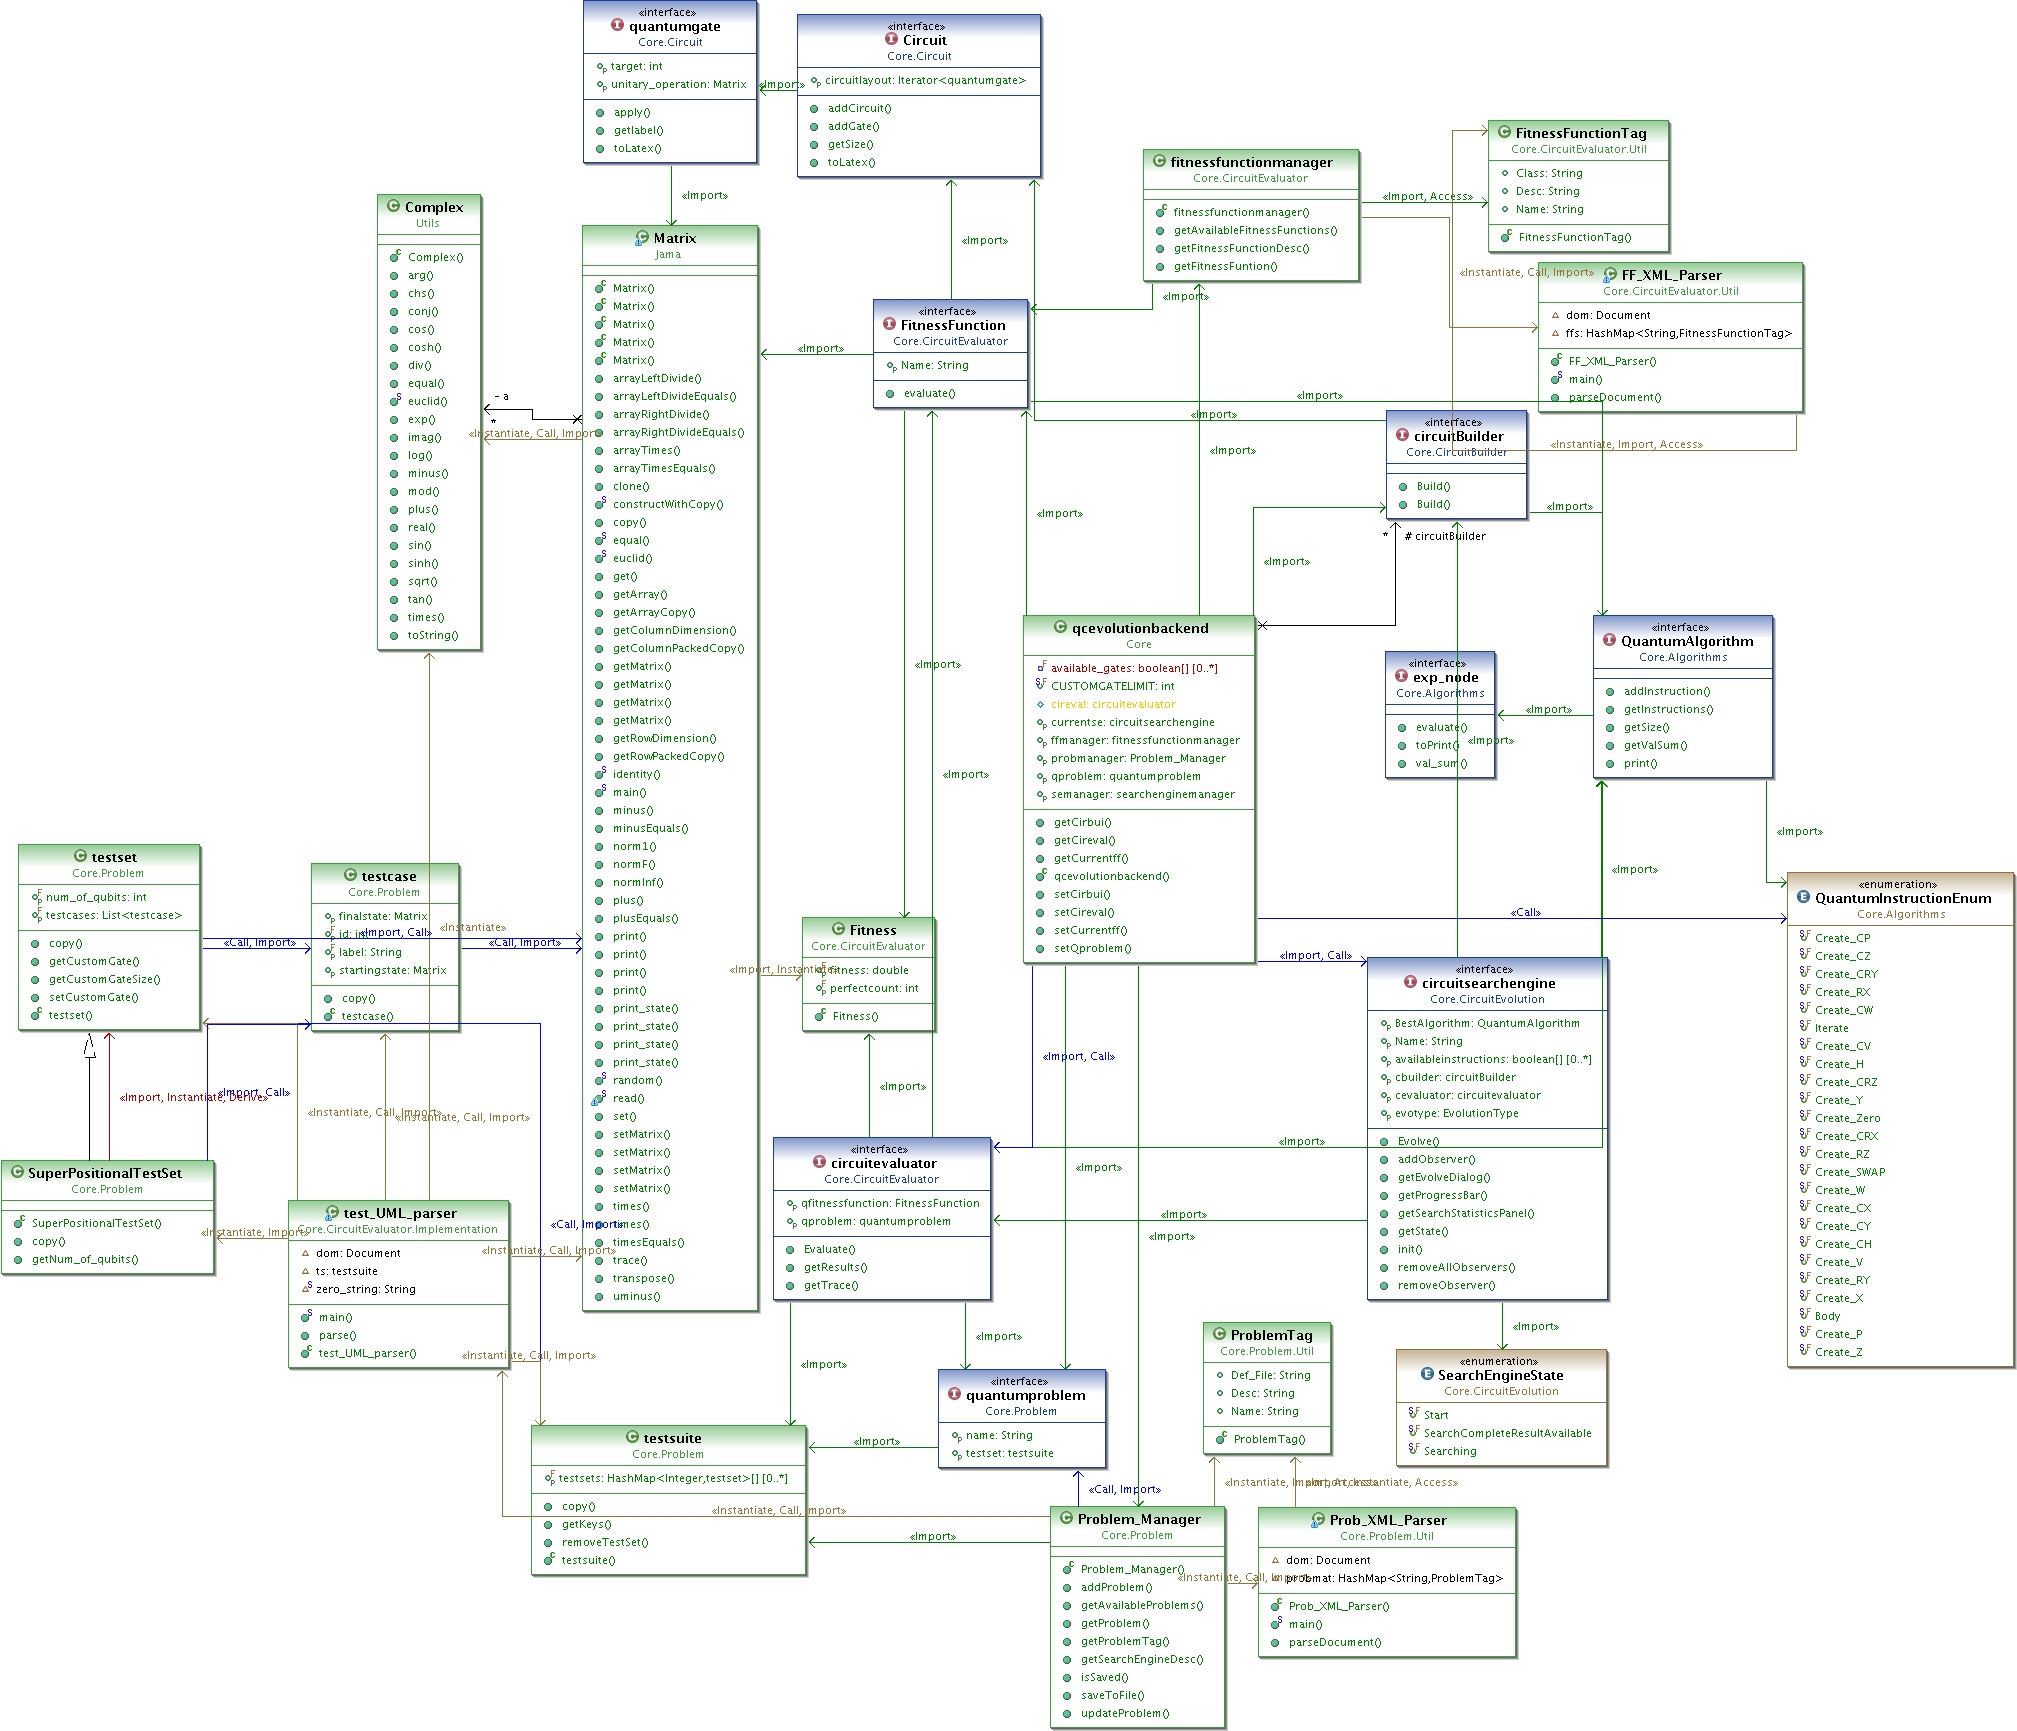
\includegraphics[height=0.85\textheight]{highlevelarchitecture.jpg}
\cleardoublepage
\endgroup

\chapter{XML Outlines}
\section{Search Engine XML Outline}
\label{sec:semanspecxml}
\lstset{language = XML}
\begin{lstlisting}
 <searchengine>
	<se>
	  <Name>SEARCH ENGINE NAMES</Name>
	  <Class>IMPLEMENTING FULLY QUALIFIED CLASS NAME</Class>
	  <Desc>SEARCH ENGINE DESCRIPTION</Desc>
	</se>
</searchengine>
\end{lstlisting}

\section{Problem Definition XML Outline}
\label{sec:probmanspecxml}
\lstset{language = XML}
\begin{lstlisting}
<Problems>
	<prob>
	  <Name>PROBLEM NAME</Name>
	  <DefFile>PROBLEM DEFINITION FILE</DefFile>
	  <Desc>PROBLEM DESCRIPTION</Desc>
	</prob>
</Problems>
\end{lstlisting}

\clearpage
\begin{landscape}

\chapter{Available Algorithm Instructions}
\label{sec:alginstructionlist}
\centering
\begin{tabular}{|c|c|c|c|c|}
\hline
\textbf{Instruction} & \textbf{Action} & & \textbf{Instruction} & \textbf{Action}  \\
\hline
\textbf{Create\_H} & Create a Hadamard Gate & & \textbf{Create\_CH} & Create a Controlled Hadamard Gate \\
\hline
\textbf{Create\_X} & Create a Pauli-X Gate & & \textbf{Create\_CX} & Create a Controlled Pauli-X Gate \\
\hline
\textbf{Create\_Y} & Create a Pauli-Y Gate & & \textbf{Create\_CY} & Create a Controlled Pauli-Y Gate \\
\hline
\textbf{Create\_Z} & Create a Pauli-Z Gate & & \textbf{Create\_CZ} & Create a Controlled Pauli-Z Gate \\
\hline
\textbf{Create\_P} & Create a Phase Gate & & \textbf{Create\_CP} & Create a Controlled Phase Gate \\
\hline
\textbf{Create\_V} & Create a V Gate & & \textbf{Create\_CV} & Create a Controlled V Gate \\
\hline
\textbf{Create\_W} & Create a W Gate & & \textbf{Create\_CW} & Create a Controlled W Gate \\
\hline
\textbf{Create\_RX} & Create a Rotate-X Gate & & \textbf{Create\_CRX} & Create a Controlled Rotate-X Gate \\
\hline
\textbf{Create\_RY} & Create a Rotate-Y Gate & & \textbf{Create\_CRY} & Create a Controlled Rotate-Y Gate \\
\hline
\textbf{Create\_RZ} & Create a Rotate-Z Gate & & \textbf{Create\_CRZ} & Create a Controlled Rotate-Z Gate \\
\hline
\textbf{Create\_SWAP} & Create a SWAP Gate & &  &  \\
\hline
\textbf{Iterate} & Run Sub-Algorithm$[0]$ for $n$ iterations & & \textbf{RevIterate} & Run Sub-Algorithm$[0]$ for $n$ iterations in reverse order\\
\hline
\textbf{Body} & Perform each Sub-Algorithm in turn & & & \\
\hline
\textbf{Create\_Custom1} & Create Custom Gate Number $1$ & & \textbf{Create\_CCustom1} & Create a Controlled Custom Gate Number $1$ \\
\hline
\textbf{Create\_Custom2} & Create Custom Gate Number $2$ & & \textbf{Create\_CCustom2} & Create a Controlled Custom Gate Number $2$ \\
\hline
\textbf{Create\_Custom3} & Create Custom Gate Number $3$ & & \textbf{Create\_CCustom3} & Create a Controlled Custom Gate Number $3$ \\
\hline
\end{tabular}
\clearpage
\end{landscape}

\end{empfile}
\end{document}
